%%%%%%%%%%%%%%%%%%%%%%%%%%%%%%%%%%%%%%%%%%%%%%%%%%%%%%%%%%%%%%%%%
% Contents: Main Input File of the LaTeX2e Introduction
% $Id$
%%%%%%%%%%%%%%%%%%%%%%%%%%%%%%%%%%%%%%%%%%%%%%%%%%%%%%%%%%%%%%%%%
% lshort.tex - The not so short introduction to LaTeX   
%                                                      by Tobias Oetiker
%                                                     oetiker@ee.ethz.ch
%
%                           based on LKURTZ.TEX Uni Graz & TU Wien, 1987
%-----------------------------------------------------------------------
%
% To compile lshort, you need TeX 3.x, LaTeX and makeindex
%
% The sources files of the Intro are:
%      lshort.tex (this file),
%      titel.tex, contrib.tex, biblio.tex
%      things.tex, typeset.tex, math.tex, lssym.tex, spec.tex,
%      lshort.sty, fancyheadings.sty
%
% Further the  verbatim.sty and the layout.sty 
% from the LaTeX Tools distribution is
% required.
%
%
% To print the AMS symbols you need the AMS fonts and the packages
% amsfonts, eufrak and eucal from (AMS LaTeX 1.2)
%
% ---------------------------------------------------------------------

%%%%%%%%%%%%%%%%%%%%%%%%%%%%%%%%%%%%%%%%%%%%%%%%%%%%%%%%%%%%%%%%%
% Contents: Who contributed to this Document
% $Id$
%%%%%%%%%%%%%%%%%%%%%%%%%%%%%%%%%%%%%%%%%%%%%%%%%%%%%%%%%%%%%%%%%
\begin{small} 
  \noindent Copyright \copyright 1995-2010 Tobias Oetiker and Contributors.  All rights reserved.
 
  This document is free; you can redistribute it and/or modify it
  under the terms of the GNU General Public License as published by
  the Free Software Foundation; either version 2 of the License, or
  (at your option) any later version.
  
  This document is distributed in the hope that it will be useful, but
  \emph{without any warranty}; without even the implied warranty of
  \emph{merchantability} or \emph{fittness for a particular purpose}\@.  See the GNU
  General Public License for more details.
  
  You should have received a copy of the GNU General Public License
  along with this document; if not, write to the Free Software
  Foundation, Inc., 675 Mass Ave, Cambridge, MA 02139, USA.

\end{small}

\chapter{Thank you!}
\noindent Much of the material used in this introduction comes from an
Austrian introduction to \LaTeX\ 2.09 written in German by:
\begin{verse}
\contrib{Hubert Partl}{partl@mail.boku.ac.at}%
{Zentraler Informatikdienst der Universit\"at f\"ur Bodenkultur Wien}
\contrib{Irene Hyna}{Irene.Hyna@bmwf.ac.at}%
   {Bundesministerium f\"ur Wissenschaft und Forschung Wien}
\contrib{Elisabeth Schlegl}{no email}%
   {in Graz}
\end{verse}

If you are interested in the German document, you can find a version
updated for \LaTeXe{} by J\"org Knappen at
\CTAN|info/lshort/german|

\newpage \noindent The
following individuals helped with corrections, suggestions and
material to improve this paper. They put in a big effort to help me
get this document into its present shape. I would like to
sincerely thank all of them. Naturally, all the mistakes you'll find
in this book are mine. If you ever find a word that is spelled
correctly, it must have been one of the people below dropping me a
line.

{ \flushleft\small
Eric~Abrahamsen,        %eric@ericabrahamsen.net
Rosemary~Bailey,        %r.a.bailey@qmw.ac.uk 0.2
Marc~Bevand,            % <bevand_m@epita.fr>
Friedemann~Brauer,      %fbrauer@is.dal.ca 3.4
Barbara~Beeton,         %bnb@ams.org
Salvatore~Bonaccorso,   % bonaccos@ee.ethz.ch
Jan~Busa,               % <busaj@ccsun.tuke.sk>
Markus~Br\"uhwiler,     % <m.br@switzerland.org>
Pietro~Braione,         % <braione@elet.polimi.it>
David~Carlisle,         %GONE carlisle@cs.man.ac.uk 1.0
Jos\'e~Carlos~Santos,   % <jcsantos@fc.up.pt>
Neil~Carter,            % N.Carter@Swansea.ac.uk
Mike~Chapman,           %chapman@eeh.ee.ethz.ch 3.16
Pierre~Chardaire,       % <pc@sys.uea.ac.uk
Christopher~Chin,       %chris.chin@rmit.edu.au 3.1
Carl~Cerecke,           %cdc@cosc.canterbury.ac.nz>
Chris~McCormack,        %GONE chrismc@eecs.umich.edu 0.1
Diego~Clavadetscher,    % DC@clavatax.ch
Wim~van~Dam,            %GONE wimvdam@cs.kun.nl 2.2
Benjamin~Deschwanden    % vdeschwb@student.ethz.ch
Jan~Dittberner,         %jan@jan-dittberner.de 3.15
Michael~John~Downes,    %<mjd@ams.org> 14 Oct 1999
Matthias~Dreier,        %dreier@ostium.ch
David~Dureisseix,       %dureisse@lmt.ens-cachan.fr 1.1
Eilinger~August,        % <eaugust@student.ethz.ch>
Elliot,                 %GONE enh-a@minster.york.ac.uk 1.1
Rockrush~Engch,         %niatlantice@gmail.com
Hans~Ehrbar,            %ehrbar@econ.utah.edu
Daniel~Flipo,           %Daniel.Flipo@univ-lille1.fr
David~Frey,             %david@eos.lugs.ch 2.2
Hans~Fugal,             %hans@fugal.net
Robert~Funnell,         %<robert.funnell@mcgill.ca>
Robin~Fairbairns,       %Robin.Fairbairns@cl.cam.ac.uk 0.2 1.0
J\"org~Fischer,        %j.fischer@xpoint.at 3.16
Erik~Frisk,             %frisk@isy.liu.se 3.4
Mic~Milic~Frederickx,   % <mic.milic@web.de>
Frank,                  %frank@freezone.co.uk 11 Feb 2000
Kasper~B.~Graversen,    % <kbg@dkik.dk>
Arlo~Griffiths,         % <A.Griffiths@let.leidenuniv.nl>
Alexandre~Guimond,      %guimond@IRO.UMontreal.CA 0.9
Andy~Goth,              % <unununium@openverse.com>
Cyril~Goutte,           %goutte@ei.dtu.dk 2.1 2.2
Greg~Gamble,            %gregg@maths.uwa.edu.au 2.2
Frank~Fischli,          % <fischlifaenger@gmx.ch>
Morten~H�gholm,		% morten.hoegholm@latex-project.org
Neil~Hammond,           %nfh@dmu.ac.uk 0.3
Rasmus~Borup~Hansen,    %GONE rbhfamos@math.ku.dk 0.2 0.9 0.91 0.92 1.9.9
Joseph~Hilferty,        % <hilferty@fil.ub.es>
Bj\"orn Hvittfeldt,     %bjorn@hvittfeldt.com 3.13
Martien~Hulsen,         %M.A.Hulsen@WbMt.TUDelft.NL 1.0 1.1
Werner~Icking,          %<Werner.Icking@gmd.de> 3.1
Jakob,                  %diness@get2net.dk
Eric~Jacoboni,          %GONE jacoboni@enseeiht.fr 0.1 0.9
Alan~Jeffrey,           %alanje@cogs.sussex.ac.uk 0.2
Byron~Jones,            %bj@dmu.ac.uk 1.1
David~Jones,            %GONE djones@CA.McMaster.dcss.insight 1.1
Nils~Kanning,           % <nils@kanning.de>
Tobias~Krewer,          %tobias.krewer@googlemail.com
Johannes-Maria~Kaltenbach, %<kaltenbach@zeiss.de> 3.01
Andrzej~Kawalec,        %GONE akawalec@prz.rzeszow.pl 1.9.9
Sander~de~Kievit,       %Skievit@ucu.uu.nl
Alain~Kessi,            %ALAIN_KESSI@HOTMAIL.COM 2.2
Christian~Kern,         %ck@unixen.hrz.uni-oldenburg.de 2.1
Tobias~Klauser,		%tklauser@access.unizh.ch 4.17
J\"org~Knappen,         %knappen@vkpmzd.kph.uni-mainz.de 0.1
Kjetil~Kjernsmo,        %<kjetil.kjernsmo@astro.uio.no> 3.2
Michael~Koundouros,     % <mkoundouros@hotmail.com>
Matt~Kraai,             % <Matt.Kraai@amo.abbott.com>
Maik~Lehradt,           %greek@uni-paderborn.de 0.1
R\'emi~Letot,           % <r_letot@yahoo.com>
Flori~Lambrechts,       % <f.lambrechts@softhome.net>
Mike~Lee,               % rmrstar@gmail.com
Axel~Liljencrantz,	% <Axel.Liljencrantz@byv.kth.se>
Johan~Lundberg,         %p99jlu@physto.se
Alexander~Mai,          %Alexander.Mai@physik.tu-darmstadt.de 3.8
Hendrik~Maryns,         %hendrik.maryns@ugent.be
Martin~Maechler,        %<maechler@stat.math.ethz.ch> 2.2
Aleksandar~S~Milosevic, % <aleksandar.milosevic@yale.edu>
Henrik~Mitsch,          % <Henrik.Mitsch@gmx.at>
Claus~Malten,           %GONE <ASI138%BITNET.DJUKFA11@BITNET.CEARN> 1.1
Kevin~Van~Maren,        % <vanmaren@fast.cs.utah.edu>  24 Nov 1999
Stefan~M.~Moser,        % stefan.moser@ieee.org 
Richard~Nagy,           % r.nagy@nameshield.net
Philipp~Nagele,         % Philipp.Nagele@t-systems.com
Lenimar~Nunes~de~Andrade, % <lenimar@mat.ufpb.br> Fri, 12 Nov 1999
I.~J.~Vera~Mar\'un,    % I.J.Veramarun@ewi.utwente.nl
Manuel~Oetiker,         % manuel@oetiker.ch
Urs~Oswald,             % osurs@bluewin.ch
Lan~Thuy~Pham,          %<lan.thuy.pham@gmail.com>
Martin~Pfister,		% m@rtinpfister.ch
Breno~Pietracci,        % <bpietracci@gmail.com>
Demerson~Andre~Polli,   % polli@linux.ime.usp.br
Nikos~Pothitos,		% <n.pothitos@di.uoa.gr>
Maksym~Polyakov         % <polyama@myrealbox.com>
Hubert~Partl,           %partl@mail.boku.ac.at 0.2 1.1
John~Refling,           %refling@sierra.lbl.gov 0.1 0.9
Mike~Ressler,           %ressler@cougar.jpl.nasa.gov 0.1 0.2 0.9 1.0 1.9.9
Brian~Ripley,           %ripley@stats.ox.ac.uk 2.1
Young~U.~Ryu,           %ryoung@utdallas.edu 2.1
Bernd~Rosenlecher,      %9rosenle@informatik.uni-hamburg.de 10 Feb 2000
Kurt~Rosenfeld,		%kurt@isis.poly.edu
Chris~Rowley,           %C.A.Rowley@open.ac.uk 0.91
Axel~Kielhorn,          % a.kielhorn@web.de
Risto~Saarelma,         %risto.saarelma@cs.helsinki.fi
Jordi~Serra~i~Solanich, %solanich@gmail.com
Hanspeter~Schmid,       %schmid@isi.ee.ethz.ch
Craig~Schlenter,        %cschle@lucy.ee.und.ac.za 0.1 0.2 0.9
Gilles~Schintgen,       %gschintgen@internet.lu
Baron~Schwartz,         % <bps7j@cs.virginia.edu>      
Christopher~Sawtell,    %<csawtell@xtra.co.nz> 1 Sep 1999
Miles~Spielberg,        %zeibach@hotmail.com
Matthieu~Stigler,       % table row height
Geoffrey~Swindale,      % <geofftswin@ntlworld.com>
Laszlo~Szathmary,       % <szathml@delfin.klte.hu>
Andr{\'a}s~Salamon,        % Andras.Salamon@comlab.ox.ac.uk
Boris~Tobotras,         % <tobotras@jet.msk.su>
Josef~Tkadlec,          %tkadlec@math.feld.cvut.cz 2.0 2.2
Scott~Veirs,            %scottv@ocean.washington.edu
Didier~Verna,           %verna@inf.enst.fr 2.2
Fabian~Wernli,          %wernli@iap.fr 3.2
Carl-Gustav~Werner,     % <Carl-Gustav.Werner@math.lu.se> 11 Oct 1999,3.16
David~Woodhouse,        % <dwmw2@infradead.org> 3.16
Chris~York,             % <c.s.york@Cummins.com>  21 Nov 1999
Fritz~Zaucker,          %zaucker@ee.ethz.ch 3.0
Rick~Zaccone,           %zaccone@bucknell.edu 2.2
and Mikhail~Zotov.      %zotov@eas.npi.msu.su 3.1

}

\vspace*{\stretch{1}}



\pagebreak
\endinput
%

% Local Variables:
% TeX-master: "lshort2e"
% mode: latex
% mode: flyspell
% End:

%%%%%%%%%%%%%%%%%%%%%%%%%%%%%%%%%%%%%%%%%%%%%%%%%%%%%%%%%%%%%%%%%
% Contents: Who contributed to this Document
% $Id$
%%%%%%%%%%%%%%%%%%%%%%%%%%%%%%%%%%%%%%%%%%%%%%%%%%%%%%%%%%%%%%%%%

% Because this introduction is the reader's first impression, I have
% edited very heavily to try to clarify and economize the language.
% I hope you do not mind! I always try to ask "is this word needed?"
% in my own writing but I don't want to impose my style on you...
% but here I think it may be more important than the rest of the book.
% --baron

\chapter{Preface}

\LaTeX{} \cite{manual} is a typesetting system that is very
suitable for producing scientific and mathematical documents of high
typographical quality. It is also suitable for producing all
sorts of other documents, from simple letters to complete books.
\LaTeX{} uses \TeX{} \cite{texbook} as its formatting engine.

This short introduction describes \LaTeXe{} and should be sufficient
for most applications of \LaTeX. Refer to~\cite{manual,companion} for
a complete description of the \LaTeX{} system.

\bigskip
\noindent This introduction is split into 6 chapters:
\begin{description}
\item[Chapter 1] tells you about the basic structure of \LaTeXe{}
  documents. You will also learn a bit about the history of \LaTeX{}.
  After reading this chapter, you should have a rough understanding how
  \LaTeX{} works.
\item[Chapter 2] goes into the details of typesetting your
  documents. It explains most of the essential \LaTeX{} commands and
  environments. After reading this chapter, you will be able to write
  your first documents, with itemized lists, tables, graphics and floating bodies.
\item[Chapter 3] explains how to typeset formulae with \LaTeX. Many
  examples demonstrate how to use one of \LaTeX{}'s
  main strengths. At the end of the chapter are tables listing
  all mathematical symbols available in \LaTeX{}.
\item[Chapter 4] explains indexes,  bibliography generation and some finer points about creating PDFs.
\item[Chapter 5] shows how to use \LaTeX{} for creating graphics. Instead
  of drawing a picture with some graphics program, saving it to a file and
  then including it into \LaTeX{}, you describe the picture and have \LaTeX{}
  draw it for you.
\item[Chapter 6] contains some potentially dangerous information about
  how to alter the
  standard document layout produced by \LaTeX{}. It will tell you how  to
  change things such that the beautiful output of \LaTeX{}
  turns ugly or stunning, depending on your abilities.
\end{description}
\bigskip
\noindent It is important to read the chapters in order---the book is
not that big, after all. Be sure to carefully read the examples,
because a lot of the information is in the
examples placed throughout the book.

\bigskip
\noindent \LaTeX{} is available for most computers, from the PC and Mac to large
UNIX and VMS systems. On many university computer clusters you will
find that a \LaTeX{} installation is available, ready to use.
Information on how to access
the local \LaTeX{} installation should be provided in the \guide. If
you have problems getting started, ask the person who gave you this
booklet. The scope of this document is \emph{not} to tell you how to
install and set up a \LaTeX{} system, but to teach you how to write
your documents so that they can be processed by~\LaTeX{}.

\bigskip
\noindent If you need to get hold of any \LaTeX{} related material,
have a look at one of the Comprehensive \TeX{} Archive Network
(CTAN) sites. The homepage is at
\url{http://www.ctan.org}.

You will find other references to CTAN throughout the book, especially
pointers to software and documents you might want to download. Instead
of writing down complete URLs, I just wrote \texttt{CTAN:} followed by
whatever location within the CTAN tree you should go to.

If you want to run \LaTeX{} on your own computer, take a look at what
is available from \CTAN|systems|.

\vspace{\stretch{1}}
\noindent If you have ideas for something to be
added, removed or altered in this document, please let me know. I am
especially interested in feedback from \LaTeX{} novices about which
bits of this intro are easy to understand and which could be explained
better.

\bigskip
\begin{verse}
\contrib{Tobias Oetiker}{tobi@oetiker.ch}%
\noindent{OETIKER+PARTNER AG\\Aarweg 15\\4600 Olten\\Switzerland}
\end{verse}
\vspace{\stretch{1}}
\noindent The current version of this document is available on\\
\CTAN|info/lshort|

\endinput



%

% Local Variables:
% TeX-master: "lshort2e"
% mode: latex
% mode: flyspell
% End:

\tableofcontents
\listoffigures
\listoftables
\enlargethispage{\baselineskip}
\mainmatter
%%%%%%%%%%%%%%%%%%%%%%%%%%%%%%%%%%%%%%%%%%%%%%%%%%%%%%%%%%%%%%%%%
% Contents: Things you need to know
% $Id$
%%%%%%%%%%%%%%%%%%%%%%%%%%%%%%%%%%%%%%%%%%%%%%%%%%%%%%%%%%%%%%%%%

\chapter{Things You Need to Know}
\begin{intro}
The first part of this chapter presents a short
overview of the philosophy and history of \LaTeXe. The second part
focuses on the basic structures of a \LaTeX{} document.
After reading this chapter, you should have a rough knowledge
of how \LaTeX{} works, which you will need to understand the rest
of this book.
\end{intro}

\section{A Bit of History}
\subsection{\TeX}

\TeX{} is a computer program created by \index{Knuth, Donald E.}Donald
E. Knuth \cite{texbook}. It is aimed at typesetting text and
mathematical formulae. Knuth started writing the \TeX{} typesetting
engine in 1977 to explore the potential of the digital printing
equipment that was beginning to infiltrate the publishing industry at
that time, especially in the hope that he could reverse the trend of
deteriorating typographical quality that he saw affecting his own
books and articles. \TeX{} as we use it today was released in 1982,
with some slight enhancements added in 1989 to better support 8-bit
characters and multiple languages. \TeX{} is renowned for being
extremely stable, for running on many different kinds of computers,
and for being virtually bug free. The version number of \TeX{} is
converging to $\pi$ and is now at $3.141592653$.


\TeX{} is pronounced ``Tech,'' with a ``ch'' as in the German word
``Ach''\footnote{In german there are actually two pronunciations for ``ch''
and one might assume that the soft ``ch'' sound from ``Pech'' would be a
more appropriate. Asked about this, Knuth wrote in the German Wikipedia:
\emph{I do not get angry when people pronounce \TeX{} in their favorite way
\ldots{} and in Germany many use a soft ch because the X follows the vowel
e, not the harder ch that follows the vowel a. In Russia, `tex' is a very
common word, pronounced `tyekh'. But I believe the most proper pronunciation
is heard in Greece, where you have the harsher ch of ach and Loch.}}
or in the Scottish ``Loch.'' The ``ch'' originates from the Greek
alphabet where X is the letter ``ch'' or ``chi''. \TeX{} is also the first syllable
of the Greek word technique. In an ASCII environment, \TeX{}
becomes \texttt{TeX}.

\subsection{\LaTeX}

\LaTeX{} enables authors to typeset and print their work at the highest
typographical quality, using a predefined, professional layout. \LaTeX{} was
originally written by \index{Lamport, Leslie}Leslie Lamport~\cite{manual}.
It uses the \TeX{} formatter as its typesetting engine. These days \LaTeX{}
is maintained by \index{The \LaTeX{} Project}the \LaTeX{} Project.

%In 1994 the \LaTeX{} package was updated by the \index{LaTeX3@\LaTeX
%  3}\LaTeX 3 team, led by \index{Mittelbach, Frank}Frank Mittelbach,
%to include some long-requested improvements, and to re\-unify all the
%patched versions which had cropped up since the release of
%\index{LaTeX 2.09@\LaTeX{} 2.09}\LaTeX{} 2.09 some years earlier. To
%distinguish the new version from the old, it is called \index{LaTeX
%2e@\LaTeXe}\LaTeXe. This documentation deals with \LaTeXe. These days you
%might be hard pressed to find the venerable \LaTeX{} 2.09 installed
%anywhere.

\LaTeX{} is pronounced ``Lay-tech'' or ``Lah-tech.'' If you refer to
\LaTeX{} in an ASCII environment, you type \texttt{LaTeX}.
\LaTeXe{} is pronounced ``Lay-tech two e'' and typed \texttt{LaTeX2e}.

%Figure~\ref{components} above % on page \pageref{components}
%shows how \TeX{} and \LaTeXe{} work together. This figure is taken from
%\texttt{wots.tex} by Kees van der Laan.

%\begin{figure}[btp]
%\begin{lined}{0.8\textwidth}
%\begin{center}
%\input{kees.fig}
%\end{center}
%\end{lined}
%\caption{Components of a \TeX{} System.} \label{components}
%\end{figure}

\section{Basics}

\subsection{Author, Book Designer, and Typesetter}

To publish something, authors give their typed manuscript to a
publishing company. One of their book designers then
decides the layout of the document (column width, fonts, space before
and after headings,~\ldots). The book designer writes his instructions
into the manuscript and then gives it to a typesetter, who typesets the
book according to these instructions.

A human book designer tries to find out what the author had in mind
while writing the manuscript. He decides on chapter headings,
citations, examples, formulae, etc.\ based on his professional
knowledge and from the contents of the manuscript.

In a \LaTeX{} environment, \LaTeX{} takes the role of the book
designer and uses \TeX{} as its typesetter. But \LaTeX{} is ``only'' a
program and therefore needs more guidance. The author has to provide
additional information to describe the logical structure of his
work. This information is written into the text as ``\LaTeX{}
commands.''

This is quite different from the \wi{WYSIWYG}\footnote{What you see is
  what you get.} approach that most modern word processors, such as
\emph{MS Word} or \emph{LibreOffice}, take. With these
applications, authors specify the document layout interactively while
typing text into the computer. They can see on the
screen how the final work will look when it is printed.

When using \LaTeX{} it is not normally possible to see the final output
while typing the text, but the final output can be previewed on the
screen after processing the file with \LaTeX. Then corrections can be
made before actually sending the document to the printer.

\subsection{Layout Design}

Typographical design is a craft. Unskilled authors often commit
serious formatting errors by assuming that book design is mostly a
question of aesthetics---``If a document looks good artistically,
it is well designed.'' But as a document has to be read and not hung
up in a picture gallery, the readability and understandability is
much more important than the beautiful look of it.
Examples:
\begin{itemize}
\item The font size and the numbering of headings have to be chosen to make
  the structure of chapters and sections clear to the reader.
\item The line length has to be short enough not to strain
  the eyes of the reader, while long enough to fill the page
  beautifully.
\end{itemize}

With \wi{WYSIWYG} systems, authors often generate aesthetically
pleasing documents with very little or inconsistent structure.
\LaTeX{} prevents such formatting errors by forcing the author to
declare the \emph{logical} structure of his document. \LaTeX{} then
chooses the most suitable layout.

\subsection{Advantages and Disadvantages}

When people from the \wi{WYSIWYG} world meet people who use \LaTeX{},
they often discuss ``the \wi{advantages of \LaTeX{}} over a normal
word processor'' or the opposite.  The best thing to do when such
a discussion starts is to keep a low profile, since such discussions
often get out of hand. But sometimes there is no escaping \ldots

\medskip\noindent So here is some ammunition. The main advantages
of \LaTeX{} over normal word processors are the following:

\begin{itemize}

\item Professionally crafted layouts are available, which make a
  document really look as if ``printed.''
\item The typesetting of mathematical formulae is supported in a
  convenient way.
\item Users only need to learn a few easy-to-understand commands
  that specify the logical structure of a document. They almost never
  need to tinker with the actual layout of the document.
\item Even complex structures such as footnotes, references, table of
  contents, and bibliographies can be generated easily.
\item Free add-on packages exist for many typographical tasks not directly supported by basic
  \LaTeX. For example, packages are
  available to include \PSi{} graphics or to typeset
  bibliographies conforming to exact standards. Many of these add-on
  packages are described in \companion.
\item \LaTeX{} encourages authors to write well-structured texts,
  because this is how \LaTeX{} works---by specifying structure.
\item \TeX, the formatting engine of \LaTeXe, is highly portable and free.
  Therefore the system runs on almost any hardware platform
  available.

%
% Add examples ...
%
\end{itemize}

\medskip

\noindent\LaTeX{} also has some disadvantages, and I guess it's a bit
difficult for me to find any sensible ones, though I am sure other people
can tell you hundreds \texttt{;-)}

\begin{itemize}
\item \LaTeX{} does not work well for people who have sold their
  souls \ldots
\item Although some parameters can be adjusted within a predefined
  document layout, the design of a whole new layout is difficult and
  takes a lot of time.\footnote{Rumour says that this is one of the
    key elements that will be addressed in the upcoming \LaTeX 3
    system.}\index{LaTeX3@\LaTeX 3}
\item It is very hard to write unstructured and disorganized documents.
\item Your hamster might, despite some encouraging first steps, never be
able to fully grasp the concept of Logical Markup.
\end{itemize}

\section{\LaTeX{} Input Files}

The input for \LaTeX{} is a plain text file. On Unix/Linux text files are
pretty common. On windows, one would use Notepad to create a text file. It
contains the text of the document, as well as the commands that tell
\LaTeX{} how to typeset the text. If you are working with a \LaTeX{} IDE, it will contain a program for creating
\LaTeX{} input files in text format.

\subsection{Spaces}

``Whitespace'' characters, such as blank or tab, are
treated uniformly as ``\wi{space}'' by \LaTeX{}. \emph{Several
  consecutive} \wi{whitespace} characters are treated as \emph{one}
``space''.  Whitespace at the start of a line is generally ignored, and
a single line break is treated as ``whitespace''.
\index{whitespace!at the start of a line}

An empty line between two lines of text defines the end of a
paragraph. \emph{Several} empty lines are treated the same as
\emph{one} empty line. The text below is an example. On the left hand
side is the text from the input file, and on the right hand side is the
formatted output.

\begin{example}
It does not matter whether you
enter one or several     spaces
after a word.

An empty line starts a new
paragraph.
\end{example}

\subsection{Special Characters}

The following symbols are \wi{reserved characters} that either have a
special meaning under \LaTeX{} or are not available in all the fonts.
If you enter them directly in your text, they will normally not print,
but rather coerce \LaTeX{} to do things you did not intend.
\begin{code}
\verb.#  $  %  ^  &  _  {  }  ~  \ . %$
\end{code}

As you will see, these characters can be used in your documents all
the same by using a prefix backslash:

\begin{example}
\# \$ \% \^{} \& \_ \{ \} \~{}
\textbackslash
\end{example}

The other symbols and many more can be printed with special commands
in mathematical formulae or as accents. The backslash character
\textbackslash{} can \emph{not} be entered by adding another backslash
in front of it (\verb|\\|); this sequence is used for
line breaking. Use the \ci{textbackslash} command instead.

\subsection{\LaTeX{} Commands}

\LaTeX{} \wi{commands} are case sensitive, and take one of the following
two formats:

\begin{itemize}
\item They start with a \wi{backslash} \verb|\| and then have a name
 consisting of letters only. Command names are terminated by a
 space, a number or any other `non-letter.'
\item They consist of a backslash and exactly one non-letter.
\item Many commands exist in a `starred variant' where a star is appended
to the command name.
\end{itemize}

%
% \\* doesn't comply !
%

%
% Can \3 be a valid command ? (jacoboni)
%
\label{whitespace}
\hyphenation{white-spaces white-space}
\LaTeX{} ignores whitespace after commands. If you want to get a
\index{whitespace!after commands}space after a command, you have to
put either an empty parameter \verb|{}| and a blank or a special spacing command after the
command name. The empty parameter \verb|{}| stops \LaTeX{} from eating up all the white space after
the command name.

\begin{example}
New \TeX users may miss whitespaces
after a command. % renders wrong
Experienced \TeX{} users are
\TeX perts, and know how to use
whitespaces. % renders correct
\end{example}

Some commands require a \wi{parameter}, which has to be given between
\wi{curly braces} \verb|{ }| after the command name. Some commands take
\wi{optional parameters}, which are inserted after the command name in
\wi{square brackets}~\verb|[ ]|.
\begin{code}
\verb|\|\textit{command}\verb|[|\textit{optional parameter}\verb|]{|\textit{parameter}\verb|}|
\end{code}
The next examples use some \LaTeX{}
commands. Don't worry about them; they will be explained later.

\begin{example}
You can \textsl{lean} on me!
\end{example}
\begin{example}
Please, start a new line
right here!\newline
Thank you!
\end{example}

\subsection{Comments}
\index{comments}

When \LaTeX{} encounters a \verb|%| character while processing an input file,
it ignores the rest of the present line, the line break, and all
whitespace at the beginning of the next line.

This can be used to write notes into the input file, which will not show up
in the printed version.

\begin{example}
This is an % stupid
% Better: instructive <----
example: Supercal%
              ifragilist%
    icexpialidocious
\end{example}

The \texttt{\%} character can also be used to split long input lines where no
whitespace or line breaks are allowed.

For longer comments you could use the \ei{comment} environment
provided by the \pai{verbatim} package. Add the
line \verb|\usepackage{verbatim}| to the preamble of your document as
explained below to use this command.

\begin{example}
This is another
\begin{comment}
rather stupid,
but helpful
\end{comment}
example for embedding
comments in your document.
\end{example}

Note that this won't work inside complex environments, like math for example.

\section{Input File Structure}
\label{sec:structure}
When \LaTeXe{} processes an input file, it expects it to follow a
certain \wi{structure}. Thus every input file must start with the
command
\begin{code}
\verb|\documentclass{...}|
\end{code}
This specifies what sort of document you intend to write. After that,
add commands to influence the style of the whole
document, or load \wi{package}s that add new
features to the \LaTeX{} system. To load such a package you use the
command
\begin{code}
\verb|\usepackage{...}|
\end{code}

When all the setup work is done,\footnote{The area between \texttt{\bs
    documentclass} and \texttt{\bs
    begin$\mathtt{\{}$document$\mathtt{\}}$} is called the
  \emph{\wi{preamble}}.} you start the body of the text with the
command

\begin{code}
\verb|\begin{document}|
\end{code}

Now you enter the text mixed with some useful \LaTeX{} commands.  At
the end of the document you add the
\begin{code}
\verb|\end{document}|
\end{code}
command, which tells \LaTeX{} to call it a day. Anything that
follows this command will be ignored by \LaTeX.

Figure~\ref{mini} shows the contents of a minimal \LaTeXe{} file. A
slightly more complicated \wi{input file} is given in
Figure~\ref{document}.

\begin{figure}[!bp]
\begin{lined}{6cm}
\begin{verbatim}
\documentclass{article}
\begin{document}
Small is beautiful.
\end{document}
\end{verbatim}
\end{lined}
\caption{A Minimal \LaTeX{} File.} \label{mini}
\end{figure}

\begin{figure}[!bp]
\begin{lined}{10cm}
\begin{verbatim}
\documentclass[a4paper,11pt]{article}
% define the title
\author{H.~Partl}
\title{Minimalism}
\begin{document}
% generates the title
\maketitle
% insert the table of contents
\tableofcontents
\section{Some Interesting Words}
Well, and here begins my lovely article.
\section{Good Bye World}
\ldots{} and here it ends.
\end{document}
\end{verbatim}
\end{lined}
\caption[Example of a Realistic Journal Article.]{Example of a Realistic
Journal Article. Note that all the commands you see in this example will be
explained later in the introduction.} \label{document}

\end{figure}

\section{A Typical Command Line Session}

I bet you must be dying to try out the neat small \LaTeX{} input file
shown on page \pageref{mini}. Here is some help:
\LaTeX{} itself comes without a GUI or
fancy buttons to press. It is just a program that crunches away at your
input file. Some \LaTeX{} installations feature a graphical front-end where
there is a \LaTeX{} button to start compiling your input file. On other systems
there might be some typing involved, so here is how to coax \LaTeX{} into
compiling your input file on a text based system. Please note: this
description assumes that a working \LaTeX{} installation already sits on
your computer.\footnote{This is the case with most well groomed Unix
Systems, and \ldots{} Real Men use Unix, so \ldots{} \texttt{;-)}}

\begin{enumerate}
\item

  Edit/Create your \LaTeX{} input file. This file must be plain ASCII
  text.  On Unix all the editors will create just that. On Windows you
  might want to make sure that you save the file in ASCII or
  \emph{Plain Text} format.  When picking a name for your file, make
  sure it bears the extension \eei{.tex}.

\item

Open a shell or cmd window, \texttt{cd} to the directory where your input file is located and run \LaTeX{} on your input file. If successful you will end up with a
\texttt{.pdf} file. It may be necessary to run \LaTeX{} several times to get
the table of contents and all internal references right. When your input
file has a bug \LaTeX{} will tell you about it and stop processing your
input file. Type \texttt{ctrl-D} to get back to the command line.
\begin{lscommand}
\verb+xelatex foo.tex+
\end{lscommand}

\end{enumerate}


\section{The Layout of the Document}

\subsection {Document Classes}\label{sec:documentclass}

The first information \LaTeX{} needs to know when processing an
input file is the type of document the author wants to create. This
is specified with the \ci{documentclass} command.
\begin{lscommand}
\ci{documentclass}\verb|[|\emph{options}\verb|]{|\emph{class}\verb|}|
\end{lscommand}
\noindent Here \emph{class} specifies the type of document to be created.
Table~\ref{documentclasses} lists the document classes explained in
this introduction. The \LaTeXe{} distribution provides additional
classes for other documents, including letters and slides.  The
\emph{\wi{option}s} parameter customizes the behavior of the document
class. The options have to be separated by commas. The most common options for the standard document
classes are listed in
Table~\ref{options}.


\begin{table}[!bp]
\caption{Document Classes.} \label{documentclasses}
\begin{lined}{\textwidth}
\begin{description}

\item [\normalfont\texttt{article}] for articles in scientific journals, presentations,
  short reports, program documentation, invitations, \ldots
  \index{article class}
\item [\normalfont\texttt{proc}] a class for proceedings based on the article class.
  \index{proc class}
\item [\normalfont\texttt{minimal}] is as small as it can get.
It only sets a page size and a base font. It is mainly used for debugging
purposes.
  \index{minimal class}
\item [\normalfont\texttt{report}] for longer reports containing several chapters, small
  books, PhD theses, \ldots \index{report class}
\item [\normalfont\texttt{book}] for real books \index{book class}
\item [\normalfont\texttt{slides}] for slides. The class uses big sans serif
  letters. You might want to consider using the Beamer class instead.
        \index{slides class}
\end{description}
\end{lined}
\end{table}

\begin{table}[!bp]
\caption{Document Class Options.} \label{options}
\begin{lined}{\textwidth}
\begin{flushleft}
\begin{description}
\item[\normalfont\texttt{10pt}, \texttt{11pt}, \texttt{12pt}] \quad Sets the size
  of the main font in the document. If no option is specified,
  \texttt{10pt} is assumed.  \index{document font size}\index{base
    font size}
\item[\normalfont\texttt{a4paper}, \texttt{letterpaper}, \ldots] \quad Defines
  the paper size. The default size is \texttt{letterpaper}. Besides
  that, \texttt{a5paper}, \texttt{b5paper}, \texttt{executivepaper},
  and \texttt{legalpaper} can be specified.  \index{legal paper}
  \index{paper size}\index{A4 paper}\index{letter paper} \index{A5
    paper}\index{B5 paper}\index{executive paper}

\item[\normalfont\texttt{fleqn}] \quad Typesets displayed formulae left-aligned
  instead of centred.

\item[\normalfont\texttt{leqno}] \quad Places the numbering of formulae on the
  left hand side instead of the right.

\item[\normalfont\texttt{titlepage}, \texttt{notitlepage}] \quad Specifies
  whether a new page should be started after the \wi{document title}
  or not. The \texttt{article} class does not start a new page by
  default, while \texttt{report} and \texttt{book} do.  \index{title}

\item[\normalfont\texttt{onecolumn}, \texttt{twocolumn}] \quad Instructs \LaTeX{} to typeset the
  document in \wi{one column} or \wi{two column}s.

\item[\normalfont\texttt{twoside, oneside}] \quad Specifies whether double or
  single sided output should be generated. The classes
  \texttt{article} and \texttt{report} are \wi{single sided} and the
  \texttt{book} class is \wi{double sided} by default. Note that this
  option concerns the style of the document only. The option
  \texttt{twoside} does \emph{not} tell the printer you use that it
  should actually make a two-sided printout.
\item[\normalfont\texttt{landscape}] \quad Changes the layout of the document to print in landscape mode.
\item[\normalfont\texttt{openright, openany}] \quad Makes chapters begin either
  only on right hand pages or on the next page available. This does
  not work with the \texttt{article} class, as it does not know about
  chapters. The \texttt{report} class by default starts chapters on
  the next page available and the \texttt{book} class starts them on
  right hand pages.

\end{description}
\end{flushleft}
\end{lined}
\end{table}

Example: An input file for a \LaTeX{} document could start with the
line
\begin{code}
\ci{documentclass}\verb|[11pt,twoside,a4paper]{article}|
\end{code}
which instructs \LaTeX{} to typeset the document as an \emph{article}
with a base font size of \emph{eleven points}, and to produce a
layout suitable for \emph{double sided} printing on \emph{A4 paper}.
\pagebreak[2]

\subsection{Packages}
\index{package} While writing your document, you will probably find
that there are some areas where basic \LaTeX{} cannot solve your
problem. If you want to include \wi{graphics}, \wi{coloured text} or
source code from a file into your document, you need to enhance the
capabilities of \LaTeX.  Such enhancements are called packages.
Packages are activated with the
\begin{lscommand}
\ci{usepackage}\verb|[|\emph{options}\verb|]{|\emph{package}\verb|}|
\end{lscommand}
\noindent command, where \emph{package} is the name of the package and
\emph{options} is a list of keywords that trigger special features in
the package. The \ci{usepackage} command goes into the preamble of the
document. See section \ref{sec:structure} for details.

Some packages come with the \LaTeXe{} base distribution
(See Table~\ref{packages}). Others are provided separately. You may
find more information on the packages installed at your site in your
\guide. The prime source for information about \LaTeX{} packages is \companion.
It contains descriptions on hundreds of packages, along with
information of how to write your own extensions to \LaTeXe.

Modern \TeX{} distributions come with a large number of packages
preinstalled. If you are working on a Unix system, use the command
\texttt{texdoc} for accessing package documentation.


\begin{table}[btp]
\caption{Some of the Packages Distributed with \LaTeX.} \label{packages}
\begin{lined}{\textwidth}
\begin{description}
\item[\normalfont\pai{doc}] Allows the documentation of \LaTeX{} programs.\\
 Described in \texttt{doc.dtx}\footnote{This file should be installed
   on your system, and you should be able to get a \texttt{dvi} file
   by typing \texttt{latex doc.dtx} in any directory where you have
   write permission. The same is true for all the
   other files mentioned in this table.}  and in \companion.

\item[\normalfont\pai{exscale}] Provides scaled versions of the
  math extension  font.\\
  Described in \texttt{ltexscale.dtx}.

\item[\normalfont\pai{fontenc}] Specifies which \wi{font encoding}
  \LaTeX{} should use.\\
  Described in \texttt{ltoutenc.dtx}.

\item[\normalfont\pai{ifthen}] Provides commands of the form\\
  `if\ldots then do\ldots otherwise do\ldots.'\\ Described in
  \texttt{ifthen.dtx} and \companion.

\item[\normalfont\pai{latexsym}] To access the \LaTeX{} symbol
  font, you should use the \texttt{latexsym} package. Described in
  \texttt{latexsym.dtx} and in \companion.

\item[\normalfont\pai{makeidx}] Provides commands for producing
  indexes.  Described in section~\ref{sec:indexing} and in \companion.

\item[\normalfont\pai{syntonly}] Processes a document without
  typesetting it.

\item[\normalfont\pai{inputenc}] Allows the specification of an
  input encoding such as ASCII, ISO Latin-1, ISO Latin-2, 437/850 IBM
  code pages,  Apple Macintosh, Next, ANSI-Windows or user-defined one.
  Described in \texttt{inputenc.dtx}.
\end{description}
\end{lined}
\end{table}


\subsection{Page Styles}

\LaTeX{} supports three predefined \wi{header}/\wi{footer}
combinations---so-called \wi{page style}s. The \emph{style} parameter
of the \index{page style!plain@\texttt{plain}}\index{plain@\texttt{plain}}
\index{page style!headings@\texttt{headings}}\index{headings@texttt{headings}}
\index{page style!empty@\texttt{empty}}\index{empty@\texttt{empty}}
\begin{lscommand}
\ci{pagestyle}\verb|{|\emph{style}\verb|}|
\end{lscommand}
\noindent command defines which one to use.
Table~\ref{pagestyle}
lists the predefined page styles.

\begin{table}[!hbp]
\caption{The Predefined Page Styles of \LaTeX.} \label{pagestyle}
\begin{lined}{\textwidth}
\begin{description}

\item[\normalfont\texttt{plain}] prints the page numbers on the bottom
  of the page, in the middle of the footer. This is the default page
  style.

\item[\normalfont\texttt{headings}] prints the current chapter heading
  and the page number in the header on each page, while the footer
  remains empty.  (This is the style used in this document)
\item[\normalfont\texttt{empty}] sets both the header and the footer
  to be empty.

\end{description}
\end{lined}
\end{table}

It is possible to change the page style of the current page
with the command
\begin{lscommand}
\ci{thispagestyle}\verb|{|\emph{style}\verb|}|
\end{lscommand}
A description how to create your own
headers and footers can be found in \companion{} and in section~\ref{sec:fancy} on page~\pageref{sec:fancy}.
%
% Pointer to the Fancy headings Package description !
%

\section{Files You Might Encounter}

When you work with \LaTeX{} you will soon find yourself in a maze of
files with various \wi{extension}s and probably no clue. The following
list explains the various \wi{file types} you might encounter when
working with \TeX{}. Please note that this table does not claim to be
a complete list of extensions, but if you find one missing that you
think is important, please drop me a line.

\begin{description}

\item[\eei{.tex}] \LaTeX{} or \TeX{} input file. Can be compiled with
  \texttt{latex}.
\item[\eei{.sty}] \LaTeX{} Macro package. Load this
  into your \LaTeX{} document using the \ci{usepackage} command.
\item[\eei{.dtx}] Documented \TeX{}. This is the main distribution
  format for \LaTeX{} style files. If you process a .dtx file you get
  documented macro code of the \LaTeX{} package contained in the .dtx
  file.
\item[\eei{.ins}] The installer for the files contained in the
  matching .dtx file. If you download a \LaTeX{} package from the net,
  you will normally get a .dtx and a .ins file. Run \LaTeX{} on the
  .ins file to unpack the .dtx file.
\item[\eei{.cls}] Class files define what your document looks
  like. They are selected with the \ci{documentclass} command.
\item[\eei{.fd}] Font description file telling  \LaTeX{} about new fonts.
\end{description}
The following files are generated when you run \LaTeX{} on your input
file:

\begin{description}
\item[\eei{.dvi}] Device Independent File. This is the main result of a classical \LaTeX{}
  compile run. Look at its content with a DVI previewer
  program or send it to a printer with \texttt{dvips} or a
  similar application. If you are using \hologo{pdfLaTeX} then you should not see any of these files.
\item[\eei{.log}] Gives a detailed account of what happened during the
  last compiler run.
\item[\eei{.toc}] Stores all your section headers. It gets read in for the
  next compiler run and is used to produce the table of contents.
\item[\eei{.lof}] This is like .toc but for the list of figures.
\item[\eei{.lot}] And again the same for the list of tables.
\item[\eei{.aux}] Another file that transports information from one
  compiler run to the next. Among other things, the .aux file is used
  to store information associated with cross-references.
\item[\eei{.idx}] If your document contains an index. \LaTeX{} stores all
  the words that go into the index in this file. Process this file with
  \texttt{makeindex}. Refer to section \ref{sec:indexing} on
  page \pageref{sec:indexing} for more information on indexing.
\item[\eei{.ind}] The processed .idx file, ready for inclusion into your
  document on the next compile cycle.
\item[\eei{.ilg}] Logfile telling what \texttt{makeindex} did.
\end{description}


% Package Info pointer
%
%



%
% Add Info on page-numbering, ...
% \pagenumbering

\section{Big Projects}
When working on big documents, you might want to split the input file
into several parts. \LaTeX{} has two commands that help you to do
that.

\begin{lscommand}
\ci{include}\verb|{|\emph{filename}\verb|}|
\end{lscommand}
\noindent Use this command in the document body to insert the
contents of another file named \emph{filename.tex}. Note that \LaTeX{}
will start a new page
before processing the material input from \emph{filename.tex}.

The second command can be used in the preamble. It allows you to
instruct \LaTeX{} to only input some of the \verb|\include|d files.
\begin{lscommand}
\ci{includeonly}\verb|{|\emph{filename}\verb|,|\emph{filename}%
\verb|,|\ldots\verb|}|
\end{lscommand}
After this command is executed in the preamble of the document, only
\ci{include} commands for the filenames that are listed in the
argument of the \ci{includeonly} command will be executed.

The \ci{include} command starts typesetting the included text on a new
page. This is helpful when you use \ci{includeonly}, because the
page breaks will not move, even when some include files are omitted.
Sometimes this might not be desirable. In this case, use the
\begin{lscommand}
\ci{input}\verb|{|\emph{filename}\verb|}|
\end{lscommand}
\noindent command. It simply includes the file specified.
No flashy suits, no strings attached.


To make \LaTeX{} quickly check your document use the \pai{syntonly}
package. This makes \LaTeX{} skim through your document only checking for
proper syntax and usage of the commands, but doesn't produce any (pdf) output.
As \LaTeX{} runs faster in this mode you may save yourself valuable time.
Usage is very simple:

\begin{verbatim}
\usepackage{syntonly}
\syntaxonly
\end{verbatim}
When you want to produce pages, just comment out the second line
(by adding a percent sign).


%

% Local Variables:
% TeX-master: "lshort2e"
% mode: latex
% mode: flyspell
% End:

%%%%%%%%%%%%%%%%%%%%%%%%%%%%%%%%%%%%%%%%%%%%%%%%%%%%%%%%%%%%%%%%%
% Contents: Typesetting Part of LaTeX2e Introduction
% $Id$
%%%%%%%%%%%%%%%%%%%%%%%%%%%%%%%%%%%%%%%%%%%%%%%%%%%%%%%%%%%%%%%%%
\chapter{Typesetting Text}

\begin{intro}
  After reading the previous chapter, you should know about the basic
  stuff of which a \LaTeXe{} document is made. In this chapter I
  will fill in the remaining structure you will need to know in order
  to produce real world material.
\end{intro}

\section{The Structure of Text and Language}
\secby{Hanspeter Schmid}{hanspi@schmid-werren.ch}
The main point of writing a text, is to convey ideas, information, or
knowledge to the reader.  The reader will understand the text better
if these ideas are well-structured, and will see and feel this
structure much better if the typographical form reflects the logical
and semantic structure of the content.

\LaTeX{} is different from other typesetting systems in that you just
have to tell it the logical and semantic structure of a text.  It
then derives the typographical form of the text according to the
``rules'' given in the document class file and in various style files.

The most important text unit in \LaTeX{} (and in typography) is the
\wi{paragraph}.  We call it ``text unit'' because a paragraph is the
typographical form that should reflect one coherent thought, or one idea.
You will learn in the following sections how to force line breaks with
e.g.\ \texttt{\bs\bs}, and paragraph breaks with e.g.\ leaving an empty line
in the source code.  Therefore, if a new thought begins, a new paragraph
should begin, and if not, only line breaks should be used.  If in doubt
about paragraph breaks, think about your text as a conveyor of ideas and
thoughts.  If you have a paragraph break, but the old thought continues, it
should be removed.  If some totally new line of thought occurs in the same
paragraph, then it should be broken.

Most people completely underestimate the importance of well-placed
paragraph breaks.  Many people do not even know what the meaning of
a paragraph break is, or, especially in \LaTeX, introduce paragraph
breaks without knowing it.  The latter mistake is especially easy to
make if equations are used in the text.  Look at the following
examples, and figure out why sometimes empty lines (paragraph breaks)
are used before and after the equation, and sometimes not.  (If you
don't yet understand all commands well enough to understand these
examples, please read this and the following chapter, and then read
this section again.)

\begin{code}
\begin{verbatim}
% Example 1
\ldots when Einstein introduced his formula
\begin{equation}
  e = m \cdot c^2 \; ,
\end{equation}
which is at the same time the most widely known
and the least well understood physical formula.


% Example 2
\ldots from which follows Kirchhoff's current law:
\begin{equation}
  \sum_{k=1}^{n} I_k = 0 \; .
\end{equation}

Kirchhoff's voltage law can be derived \ldots


% Example 3
\ldots which has several advantages.

\begin{equation}
  I_D = I_F - I_R
\end{equation}
is the core of a very different transistor model. \ldots
\end{verbatim}
\end{code}

The next smaller text unit is a sentence.  In English texts, there is
a larger space after a period that ends a sentence than after one
that ends an abbreviation.  \LaTeX{} tries to figure out which one
you wanted to have.  If \LaTeX{} gets it wrong, you must tell it what
you want.  This is explained later in this chapter.

The structuring of text even extends to parts of sentences.  Most
languages have very complicated punctuation rules, but in many
languages (including German and English), you will get almost every
comma right if you remember what it represents: a short stop in the
flow of language.  If you are not sure about where to put a comma,
read the sentence aloud and take a short breath at every comma.  If
this feels awkward at some place, delete that comma; if you feel the
urge to breathe (or make a short stop) at some other place, insert a
comma.

Finally, the paragraphs of a text should also be structured logically
at a higher level, by putting them into chapters, sections,
subsections, and so on.  However, the typographical effect of writing
e.g.\ \verb|\section{The| \texttt{Structure of Text and Language}\verb|}| is
so obvious that it is almost self-evident how these high-level
structures should be used.

\section{Line Breaking and Page Breaking}

\subsection{Justified Paragraphs}

Books are often typeset with each line having the same length.
\LaTeX{} inserts the necessary \wi{line break}s and spaces between words
by optimizing the contents of a whole paragraph. If necessary, it
also hyphenates words that would not fit comfortably on a line.
How the paragraphs are typeset depends on the document class.
Normally the first line of a paragraph is indented, and there is no
additional space between two paragraphs. Refer to section~\ref{parsp}
for more information.

In special cases it might be necessary to order \LaTeX{} to break a
line:
\begin{lscommand}
\ci{\bs} or \ci{newline}
\end{lscommand}
\noindent starts a new line without starting a new paragraph.

\begin{lscommand}
\ci{\bs*}
\end{lscommand}
\noindent additionally prohibits a page break after the forced
line break.

\begin{lscommand}
\ci{newpage}
\end{lscommand}
\noindent starts a new page.

\begin{lscommand}
\ci{linebreak}\verb|[|\emph{n}\verb|]|,
\ci{nolinebreak}\verb|[|\emph{n}\verb|]|,
\ci{pagebreak}\verb|[|\emph{n}\verb|]|,
\ci{nopagebreak}\verb|[|\emph{n}\verb|]|
\end{lscommand}
\noindent suggest places where a break may (or may not) happen. They enable the author to influence their
actions with the optional argument \emph{n}, which can be set to a number
between zero and four. By setting \emph{n} to a value below 4, you leave
\LaTeX{} the option of ignoring your command if the result would look very
bad. Do not confuse these ``break'' commands with the ``new'' commands. Even
when you give a ``break'' command, \LaTeX{} still tries to even out the
right border of the line and the total length of the page, as described in
the next section; this can lead to unpleasant gaps in your text.
If you really want to start a ``new line'' or a ``new page'', then use the
corresponding command. Guess their names!


\LaTeX{} always tries to produce the best line breaks possible. If it
cannot find a way to break the lines in a manner that meets its high
standards, it lets one line stick out on the right of the paragraph.
\LaTeX{} then complains (``\wi{overfull hbox}'') while processing the
input file. This happens most often when \LaTeX{} cannot find a
suitable place to hyphenate a word.\footnote{Although \LaTeX{} gives
  you a warning when that happens (\texttt{Overfull \bs{}hbox}) and displays the
  offending line, such lines are not always easy to find. If you use
  the option \texttt{draft} in the \ci{documentclass} command, these
  lines will be marked with a thick black line on the right margin.}
Instruct \LaTeX{} to lower its standards a little by giving
the \ci{sloppy} command. It prevents such over-long lines by
increasing the inter-word spacing---even if the final output is not
optimal.  In this case a warning (``\wi{underfull hbox}'') is given to
the user.  In most such cases the result doesn't look very good. The
command \ci{fussy} brings \LaTeX{} back to its default behaviour.

\subsection{Hyphenation} \label{hyph}

\LaTeX{} hyphenates words whenever necessary. If the hyphenation
algorithm does not find the correct hyphenation points,
remedy the situation by using the following commands to tell \TeX{}
about the exception.

The command
\begin{lscommand}
\ci{hyphenation}\verb|{|\emph{word list}\verb|}|
\end{lscommand}
\noindent causes the words listed in the argument to be hyphenated only at
the points marked by ``\verb|-|''.  The argument of the command should only
contain words built from normal letters, or rather signs that are considered
to be normal letters by \LaTeX{}. The hyphenation hints are
stored for the language that is active when the hyphenation command
occurs. This means that if you place a hyphenation command into the preamble
of your document it will influence the English language hyphenation. If you
place the command after the \verb|\begin{document}| and you are using some
package for national language support like \pai{polyglossia}, then the hyphenation
hints will be active in the language activated through \pai{polyglossia}.

The example below will allow ``hyphenation'' to be hyphenated as well as
``Hyphenation'', and it prevents ``FORTRAN'', ``Fortran'' and ``fortran''
from being hyphenated at all.  No special characters or symbols are allowed
in the argument.

Example:
\begin{code}
\verb|\hyphenation{FORTRAN Hy-phen-a-tion}|
\end{code}

The command \ci{-} inserts a discretionary hyphen into a word. This
also becomes the only point hyphenation is allowed in this word. This
command is especially useful for words containing special characters
(e.g.\ accented characters), because \LaTeX{} does not automatically
hyphenate words containing special characters.
%\footnote{Unless you are using the new
%\wi{DC fonts}.}.

\begin{example}
I think this is: su\-per\-cal\-%
i\-frag\-i\-lis\-tic\-ex\-pi\-%
al\-i\-do\-cious
\end{example}

Several words can be kept together on one line with the command
\begin{lscommand}
\ci{mbox}\verb|{|\emph{text}\verb|}|
\end{lscommand}
\noindent It causes its argument to be kept together under all circumstances.

\begin{example}
My phone number will change soon.
It will be \mbox{0116 291 2319}.

The parameter
\mbox{\emph{filename}} should
contain the name of the file.
\end{example}

\ci{fbox} is similar to \ci{mbox}, but in addition there will
be a visible box drawn around the content.


\section{Ready-Made Strings}

In some of the examples on the previous pages, you have seen
some very simple \LaTeX{} commands for typesetting special
text strings:

\vspace{2ex}

\noindent
\begin{tabular}{@{}lll@{}}
Command&Example&Description\\
\hline
\ci{today} & \today   & Current date\\
\ci{TeX} & \TeX       & Your favorite typesetter\\
\ci{LaTeX} & \LaTeX   & The Name of the Game\\
\ci{LaTeXe} & \LaTeXe & The current incarnation\\
\end{tabular}

\section{Special Characters and Symbols}

\subsection{Quotation Marks}

You should \emph{not} use the \verb|"| for \wi{quotation marks}
\index{""@\texttt{""}} as you would on a typewriter.  In publishing
there are special opening and closing quotation marks.  In \LaTeX{},
use two~\textasciigrave~(grave accent) for opening quotation marks and
two~\textquotesingle~(vertical quote) for closing quotation marks. For single
quotes you use just one of each.
\begin{example}
``Please press the `x' key.''
\end{example}
Yes I know the rendering is not ideal, it's really a back-tick or grave accent
(\textasciigrave) for
opening quotes and vertical quote (\textquotesingle) for closing, despite what the font chosen might suggest.

\subsection{Dashes and Hyphens}

\LaTeX{} knows four kinds of \wi{dash}es. Access three of
them with different number of consecutive dashes. The fourth sign
is actually not a dash at all---it is the mathematical minus sign: \index{-}
\index{--} \index{---} \index{-@$-$} \index{mathematical!minus}

\begin{example}
daughter-in-law, X-rated\\
pages 13--67\\
yes---or no? \\
$0$, $1$ and $-1$
\end{example}
The names for these dashes are:
`-' \wi{hyphen}, `--' \wi{en-dash}, `---' \wi{em-dash} and
`$-$' \wi{minus sign}.

\subsection{Tilde ($\sim$)}
\index{URL link}\index{tilde}
A character often seen in web addresses is the tilde. To generate
this in \LaTeX{} use \verb|\~{}| but the result (\~{}) is not really
what you want. Try this instead:

\begin{example}
http://www.rich.edu/\~{}bush \\
http://www.clever.edu/$\sim$demo
\end{example}

\subsection{Slash (/)}
\index{Slash}
In order to typeset a slash between two words, one can simply type e.g.\
\texttt{read/write}, but this makes \LaTeX{} treat the two words as one.
Hyphenation is disabled for these two words, so there may be `overfull'
errors.  To overcome this, use \ci{slash}.  For example type
`\verb|read\slash write|' which allows hyphenation.  But normal `\texttt{/}'
character may be still used for ratios or units, e.g.\ \texttt{5 MB/s}.

\subsection{Degree Symbol \texorpdfstring{($\circ$)}{}}

Printing the \wi{degree symbol} in pure \LaTeX{}.

\begin{example}
It's $-30\,^{\circ}\mathrm{C}$.
I will soon start to
super-conduct.
\end{example}

The \pai{textcomp} package makes the degree symbol also available as
\ci{textdegree} or in combination with the C by using the \ci{textcelsius}.

\begin{example}
30 \textcelsius{} is
86 \textdegree{}F.
\end{example}

\subsection{The Euro Currency Symbol \texorpdfstring{(\officialeuro)}{}}

When writing about money these days, you need the Euro symbol. Many current
fonts contain a Euro symbol. After loading the \pai{textcomp} package in the preamble of your document
\begin{lscommand}
\ci{usepackage}\verb|{textcomp}|
\end{lscommand}
use the command
\begin{lscommand}
\ci{texteuro}
\end{lscommand}
to access it.

If your font does not provide its own Euro symbol or if you do not like the
font's Euro symbol, you have two more choices:

First the \pai{eurosym} package. It provides the official Euro symbol:
\begin{lscommand}
\ci{usepackage}\verb|[|\emph{official}\verb|]{eurosym}|
\end{lscommand}
If you prefer a Euro symbol that matches your font, use the option
\texttt{gen} in place of the \texttt{official} option.

%If the Adobe Eurofonts are installed on your system (they are available for
%free from \url{ftp://ftp.adobe.com/pub/adobe/type/win/all}) you can use
%either the package \pai{europs} and the command \ci{EUR} (for a Euro symbol
%that matches the current font).
% does not work
% or the package
% \pai{eurosans} and the command \ci{euro} (for the ``official Euro'').

%The \pai{marvosym} package also provides many different symbols, including a
%Euro, under the name \ci{EURtm}. Its disadvantage is that it does not provide
%slanted and bold variants of the Euro symbol.

\begin{table}[!htbp]
\caption{A bag full of Euro symbols} \label{eurosymb}
\begin{lined}{10cm}
\begin{tabular}{llccc}
LM+textcomp  &\verb+\texteuro+ & \huge\texteuro &\huge\sffamily\texteuro
                                                &\huge\ttfamily\texteuro\\
eurosym      &\verb+\euro+ & \huge\officialeuro &\huge\sffamily\officialeuro
                                                &\huge\ttfamily\officialeuro\\
$[$gen$]$eurosym &\verb+\euro+ & \huge\geneuro  &\huge\sffamily\geneuro
                                                &\huge\ttfamily\geneuro\\
%europs       &\verb+\EUR + & \huge\EURtm        &\huge\EURhv
%                                                &\huge\EURcr\\
%eurosans     &\verb+\euro+ & \huge\EUROSANS  &\huge\sffamily\EUROSANS
%                                             & \huge\ttfamily\EUROSANS \\
%marvosym     &\verb+\EURtm+  & \huge\mvchr101  &\huge\mvchr101
%                                               &\huge\mvchr101
\end{tabular}
\medskip
\end{lined}
\end{table}

\subsection{Ellipsis (\texorpdfstring{\ldots}{...})}

On a typewriter, a \wi{comma} or a \wi{period} takes the same amount of
space as any other letter. In book printing, these characters occupy
only a little space and are set very close to the preceding letter.
Therefore, entering `\wi{ellipsis}' by just typing three
dots would produce the wrong result. Instead, there is a special
command for these dots. It is called

\begin{lscommand}
\ci{ldots} (low dots)
\end{lscommand}
\index{...@\ldots}


\begin{example}
Not like this ... but like this:\\
New York, Tokyo, Budapest, \ldots
\end{example}

\subsection{Ligatures}

Some letter combinations are typeset not just by setting the
different letters one after the other, but by actually using special
symbols.
\begin{code}
{\large ff fi fl ffi\ldots}\quad
instead of\quad {\large f{}f f{}i f{}l f{}f{}i \ldots}
\end{code}
These so-called \wi{ligature}s can be prohibited by inserting an \ci{mbox}\verb|{}|
between the two letters in question. This might be necessary with
words built from two words.

\begin{example}
\Large Not shelfful\\
but shelf\mbox{}ful
\end{example}

\subsection{Accents and Special Characters}

\LaTeX{} supports the use of \wi{accent}s and \wi{special character}s
from many languages. Table~\ref{accents} shows all sorts of accents
being applied to the letter o. Naturally other letters work too.

To place an accent on top of an i or a j, its dots have to be
removed. This is accomplished by typing \verb|\i| and \verb|\j|.

\begin{example}
H\^otel, na\"\i ve, \'el\`eve,\\
sm\o rrebr\o d, !`Se\~norita!,\\
Sch\"onbrunner Schlo\ss{}
Stra\ss e
\end{example}

\begin{table}[!hbp]
\caption{Accents and Special Characters.} \label{accents}
\begin{lined}{10cm}
\begin{tabular}{*4{cl}}
\mstA{\`o} & \mstA{\'o} & \mstA{\^o} & \mstA{\~o} \\
\mstA{\=o} & \mstA{\.o} & \mstA{\"o} & \mstB{\c}{c}\\[6pt]
\mstB{\u}{o} & \mstB{\v}{o} & \mstB{\H}{o} & \mstB{\c}{o} \\
\mstB{\d}{o} & \mstB{\b}{o} & \mstB{\t}{oo} \\[6pt]
\mstA{\oe}  &  \mstA{\OE} & \mstA{\ae} & \mstA{\AE} \\
\mstA{\aa} &  \mstA{\AA} \\[6pt]
\mstA{\o}  & \mstA{\O} & \mstA{\l} & \mstA{\L} \\
\mstA{\i}  & \mstA{\j} & !` & \verb|!`| & ?` & \verb|?`|
\end{tabular}
\index{dotless \i{} and \j}\index{Scandinavian letters}
\index{ae@\ae}\index{umlaut}\index{grave}\index{acute}
\index{oe@\oe}\index{aa@\aa}

\bigskip
\end{lined}
\end{table}

\section{International Language Support}
\secby{Axel Kielhorn}{A.Kielhorn@web.de}%
\index{international} When you write documents in \wi{language}s
other than English, there are three areas where \LaTeX{} has to be
configured appropriately:

\begin{enumerate}
\item All automatically generated text strings\footnote{Table of
    Contents, List of Figures, \ldots} have to be adapted to the new
  language.
\item \LaTeX{} needs to know the hyphenation rules for the current language.
\item Language specific typographic rules. In French for example, there is a
  mandatory space before each colon character (:).
\end{enumerate}

Also entering text in your language of choice might be a bit cumbersome using all the
commands from figure~\ref{accents}. To overcome this problem, until recently you had to delve
deep into the abyss of language specific encodings both for input as well as fonts. These days,
with modern \TeX{} engines speaking UTF-8 natively, these problems have relaxed considerably.

The package \pai{polyglossia}\cite{polyglossia} is a replacement for
venerable \pai{babel} package. It takes care of the hyphenation patterns and automatically
generated text strings in your documents.

The package \pai{fontspec}\cite{fontspec} handles font loading for
\hologo{XeLaTeX} and \hologo{LuaTeX}. The default font is Latin Modern
Roman.

\subsection{Polyglossia Usage}

Depending on the \TeX{} engine you use slighly different commands are
necessary in the preamble of your document to properly enable multilingual
processing. Figure~\ref{allinone} on page~\pageref{allinone} shows a sample preamble that takes care of all the necessary settings.

\begin{figure}[!bp]
\begin{lined}{10cm}
\begin{verbatim}
\usepackage{iftex}
\ifXeTeX
   \usepackage{fontspec}
\else
   \usepackage{luatextra}
\fi
\defaultfontfeatures{Ligatures=TeX}
\usepackage{polyglossia}
\end{verbatim}
\end{lined}
\caption[All in one preamble]{All in one preamble that takes care of \hologo{LuaLaTeX} and \hologo{XeLaTeX}} \label{allinone}
\end{figure}

So far there has been no advantage to using a Unicode \hologo{TeX} engine.
This changes when we leave the Latin script and move to a more interesting
language like Greek or Russian.  With a Unicode based system, you can
simply\footnote{For small values of simple.} enter the native characters in your
editor and \hologo{TeX} will understand them.

Writing in different languages is easy, just specify the languages in the
preamble. This example uses the \pai{csquotes} package which generates
the right kind of quotes according to the language you are writing in. Note
that it needs to be loaded \emph{before} loading the language support.

\begin{lscommand}
\verb|\usepackage[autostyle=true]{csquotes}|\\
\verb|\setdefaultlanguage{english}|\\
\verb|\setotherlanguage{german}|
\end{lscommand}
%
To write a paragraph in German, you can use the German environment:

\begin{example}
English text.
\begin{german}
Deutscher \enquote{Text}.
\end{german}
More English \enquote{text}.
\end{example}

If you just need a word in a foreign language you can use the
\verb|\text|\emph{language} command:

\begin{example}
Did you know that
\textgerman{Gesundheit} is
actually a German word.
\end{example}

This may look unnecessary since the only advantage is a correct hyphenation,
but when the second language is a little bit more exotic it will be worth
the effort.

Sometimes the font used in the main document does not contain glyphs that
are required in the second language. Latin Modern for example does not contain
Cyrillic letters. The solution is to define a font that will be used for
that language. Whenever a new language is activated, \pai{polyglossia} will
first check whether a font has been defined for that language. If you are happy with the computer modern font, you may want to try the \enquote{Computer Modern Unicode} font by adding the following commands to the preamble of your document.

\medskip\noindent For \hologo{LuaLaTeX} it is pretty simple
\begin{verbatim}
\setmainfont{CMU Serif}
\setsansfont{CMU Sans Serif}
\setmonofont{CMU Typewriter Text}
\end{verbatim}
\noindent For \hologo{XeLaTeX} you have to be a bit more explicit:
\begin{verbatim}
\setmainfont{cmun}[
   Extension=.otf,UprightFont=*rm,ItalicFont=*ti,
   BoldFont=*bx,BoldItalicFont=*bi,
 ]
 \setsansfont{cmun}[
   Extension=.otf,UprightFont=*ss,ItalicFont=*si,
   BoldFont=*sx,BoldItalicFont=*so,
 ]
 \setmonofont{cmun}[
   Extension=.otf,UprightFont=*btl,ItalicFont=*bto,
   BoldFont=*tb,BoldItalicFont=*tx,
 ]
\end{verbatim}

With the appropriate fonts loaded, you can now write:

\begin{example}
\textrussian{Правда} is
a russian newspaper.
\textgreek{ἀλήθεια} is truth
or disclosure in philosophy
\end{example}

The package \pai{xgreek}\index{Greek}\cite{xgreek} offers support for
writing either ancient or modern (monotonic or polytonic) greek.

\subsubsection{Right to Left (RTL) languages.}

Some languages are written left to right, others are written right to
left(RTL). \pai{polyglossia} needs the \pai{bidi}\cite{bidi}
package\footnote{\texttt{bidi} does not support \hologo{LuaTeX}.} in order
to support RTL languages. The \pai{bidi} package should be the last package
you load, even after \pai{hyperref} which is usually the last package.
(Since \pai{polyglossia} loads \pai{bidi} this means that \pai{polyglossia}
should be the last package loaded.)

The package \pai{xepersian}\index{Persian}\cite{xepersian} offers support
for the Persian language. It supplies Persian \LaTeX-commands that allows
you to enter commands like \verb|\section| in Persian, which makes this
really attractive to native speakers. \pai{xepersian} is the only package
that supports kashida\index{kashida} with \hologo{XeLaTeX}. A package for
Syriac which uses a similar algorithm is under development.

The IranNastaliq font provided by the SCICT\footnote{Supreme Council of
Information and Communication Technology} is available at their website
\url{http://www.scict.ir/Portal/Home/Default.aspx}.

The \pai{arabxetex}\cite{arabxetex} package supports several languages with
an Arabic script:

\begin{itemize}
\item arab (Arabic)\index{Arabic}
\item persian\index{Persian}
\item urdu\index{Urdu}
\item sindhi\index{Sindhi}
\item pashto\index{Pashto}
\item ottoman (turk)\index{Ottoman}\index{Turkish}
\item kurdish\index{Kurdish}
\item kashmiri\index{Kashmiri}
\item malay (jawi)\index{Malay}\index{Jawi}
\item uighur\index{Uighur}
\end{itemize}

It offers a font mapping that enables \hologo{XeLaTeX} to process input
using the Arab\TeX\ ASCII transcription.

Fonts that support several Arabic laguages are offered by the
IRMUG\footnote{Iranian Mac User Group} at
\url{http://wiki.irmug.org/index.php/X_Series_2}.

There is no package available for Hebrew\index{Hebrew} because none is
needed. The Hebrew support in \pai{polyglossia} should be sufficient. But
you do need a suitable font with real Unicode Hebrew. SBL Hebrew is free for
non-commercial use and available at
\url{http://www.sbl-site.org/educational/biblicalfonts.aspx}. Another font
available under the Open Font License is Ezra SIL, available at
\url{http://www.sil.org/computing/catalog/show_software.asp?id=76}.

Remember to select the correct script:

\begin{lscommand}
\verb|\newfontfamily\hebrewfont[Script=Hebrew]{SBL Hebrew}| \\
\verb|\newfontfamily\hebrewfont[Script=Hebrew]{Ezra SIL}|
\end{lscommand}


\subsubsection{Chinese, Japanese and Korean (CJK)}
\index{Chinese}\index{Japanese}\index{Korean}

The package \pai{xeCJK}\cite{xecjk} takes care of font selection and
punctuation for these languages.

\section{The Space Between Words}

To get a straight right margin in the output, \LaTeX{} inserts varying
amounts of space between the words. It inserts slightly more space at
the end of a sentence, as this makes the text more readable.  \LaTeX{}
assumes that sentences end with periods, question marks or exclamation
marks. If a period follows an uppercase letter, this is not taken as a
sentence ending, since periods after uppercase letters normally occur in
abbreviations.

Any exception from these assumptions has to be specified by the
author. A backslash in front of a space generates a space that will
not be enlarged. A tilde~`\verb|~|' character generates a space that cannot be
enlarged and additionally prohibits a line break. The command
\verb|\@| in front of a period specifies that this period terminates a
sentence even when it follows an uppercase letter.
\cih{"@} \index{~@ \verb.~.} \index{tilde@tilde ( \verb.~.)}
\index{., space after}

\begin{example}
Mr.~Smith was happy to see her\\
cf.~Fig.~5\\
I like BASIC\@. What about you?
\end{example}

The additional space after periods can be disabled with the command
\begin{lscommand}
\ci{frenchspacing}
\end{lscommand}
\noindent which tells \LaTeX{} \emph{not} to insert more space after a
period than after an ordinary character. This is very common in
non-English languages, except bibliographies. If you use
\ci{frenchspacing}, the command \verb|\@| is not necessary.

\section{Titles, Chapters, and Sections}

To help the reader find his or her way through your work, you should
divide it into chapters, sections, and subsections.  \LaTeX{} supports
this with special commands that take the section title as their
argument.  It is up to you to use them in the correct order.

The following sectioning commands are available for the
\texttt{article} class: \nopagebreak

\begin{lscommand}
\ci{section}\verb|{...}|\\
\ci{subsection}\verb|{...}|\\
\ci{subsubsection}\verb|{...}|\\
\ci{paragraph}\verb|{...}|\\
\ci{subparagraph}\verb|{...}|
\end{lscommand}

If you want to split your document into parts without influencing the
section or chapter numbering use
\begin{lscommand}
\ci{part}\verb|{...}|
\end{lscommand}

When you work with the \texttt{report} or \texttt{book} class,
an additional top-level sectioning command becomes available
\begin{lscommand}
\ci{chapter}\verb|{...}|
\end{lscommand}

As the \texttt{article} class does not know about chapters, it is quite easy
to add articles as chapters to a book.
The spacing between sections, the numbering and the font size of the
titles will be set automatically by \LaTeX.

Two of the sectioning commands are a bit special:
\begin{itemize}
\item The \ci{part} command does
  not influence the numbering sequence of chapters.
\item The \ci{appendix} command does not take an argument. It just
  changes the chapter numbering to letters.\footnote{For the article
    style it changes the section numbering.}
\end{itemize}

\LaTeX{} creates a table of contents by taking the section headings
and page numbers from the last compile cycle of the document. The command
\begin{lscommand}
\ci{tableofcontents}
\end{lscommand}
\noindent expands to a table of contents at the place it
is issued. A new
document has to be compiled (``\LaTeX ed'') twice to get a
correct \wi{table of contents}. Sometimes it might be
necessary to compile the document a third time. \LaTeX{} will tell you
when this is necessary.

All sectioning commands listed above also exist as ``starred''
versions.  A ``starred'' version of a command is built by adding a
star \verb|*| after the command name.  This generates section headings
that do not show up in the table of contents and are not
numbered. The command \verb|\section{Help}|, for example, would become
\verb|\section*{Help}|.

Normally the section headings show up in the table of contents exactly
as they are entered in the text. Sometimes this is not possible,
because the heading is too long to fit into the table of contents. The
entry for the table of contents can then be specified as an
optional argument in front of the actual heading.

\begin{code}
\verb|\chapter[Title for the table of contents]{A long|\\
\verb|    and especially boring title, shown in the text}|
\end{code}

The \wi{title} of the whole document is generated by issuing a
\begin{lscommand}
\ci{maketitle}
\end{lscommand}
\noindent command. The contents of the title have to be defined by the commands
\begin{lscommand}
\ci{title}\verb|{...}|, \ci{author}\verb|{...}|
and optionally \ci{date}\verb|{...}|
\end{lscommand}
\noindent before calling \verb|\maketitle|. In the argument to \ci{author}, you can supply several names separated by \ci{and} commands.

An example of some of the commands mentioned above can be found in
Figure~\ref{document} on page~\pageref{document}.

Apart from the sectioning commands explained above, \LaTeXe{}
introduced three additional commands for use with the \verb|book| class.
They are useful for dividing your publication. The commands alter
chapter headings and page numbering to work as you would expect in
a book:
\begin{description}
\item[\ci{frontmatter}] should be the very first command after
  the start of the document body (\verb|\begin{document}|). It will switch page numbering to Roman
    numerals and sections will be non-enumerated as if you were using
    the starred sectioning commands (eg \verb|\chapter*{Preface}|)
    but the sections will still show up in the table of contents.
\item[\ci{mainmatter}] comes right before the first chapter of
  the book. It turns on Arabic page numbering and restarts the page
  counter.
\item[\ci{appendix}] marks the start of additional material in your
  book. After this command chapters will be numbered with letters.
\item[\ci{backmatter}] should be inserted before the very last items
  in your book, such as the bibliography and the index. In the standard
  document classes, this has no visual effect.
\end{description}


\section{Cross References}

In books, reports and articles, there are often
\wi{cross-references} to figures, tables and special segments of text.
\LaTeX{} provides the following commands for cross referencing
\begin{lscommand}
\ci{label}\verb|{|\emph{marker}\verb|}|, \ci{ref}\verb|{|\emph{marker}\verb|}|
and \ci{pageref}\verb|{|\emph{marker}\verb|}|
\end{lscommand}
\noindent where \emph{marker} is an identifier chosen by the user. \LaTeX{}
replaces \verb|\ref| by the number of the section, subsection, figure,
table, or theorem after which the corresponding \verb|\label| command
was issued. \verb|\pageref| prints the page number of the
page where the \verb|\label| command occurred.\footnote{Note that these commands
  are not aware of what they refer to. \ci{label} just saves the last
  automatically generated number.} As with section titles and page numbers for the table of contents,
the numbers from the previous compile cycle are used.


\begin{example}
A reference to this subsection
\label{sec:this} looks like:
``see section~\ref{sec:this} on
page~\pageref{sec:this}.''
\end{example}

\section{Footnotes}
With the command
\begin{lscommand}
\ci{footnote}\verb|{|\emph{footnote text}\verb|}|
\end{lscommand}
\noindent a footnote is printed at the foot of the current page.  Footnotes
should always be put\footnote{``put'' is one of the most common
  English words.} after the word or sentence they refer to. Footnotes
referring to a sentence or part of it should therefore be put after
the comma or period.\footnote{Note that footnotes
  distract the reader from the main body of your document. After all,
  everybody reads the footnotes---we are a curious species, so why not
  just integrate everything you want to say into the body of the
  document?\footnotemark}
\footnotetext{A guidepost doesn't necessarily go where it's pointing to :-).}

\begin{example}
Footnotes\footnote{This is
  a footnote.} are often used
by people using \LaTeX.
\end{example}

\section{Emphasized Words}

If a text is typed using a typewriter, important words are
  \texttt{emphasized by \underline{underlining} them.}
\begin{lscommand}
\ci{underline}\verb|{|\emph{text}\verb|}|
\end{lscommand}
In printed books,
however, words are emphasized by typesetting them in an \emph{italic}
font.  As an author you shouldn't care either way. The important bit is, to tell \LaTeX{} that a
particular bit of text is important and should be emphasized. Hence the command
\begin{lscommand}
\ci{emph}\verb|{|\emph{text}\verb|}|
\end{lscommand}
\noindent to emphasize text. What the command actually does with
its argument depends on the context:

\begin{example}
\emph{If you use
  emphasizing inside a piece
  of emphasized text, then
  \LaTeX{} uses the
  \emph{normal} font for
  emphasizing.}
\end{example}

If you want control over font and font size, section \ref{sec:fontsize} on
page \pageref{sec:fontsize} might provide some inspiration.

\section{Environments} \label{env}

% To typeset special purpose text, \LaTeX{} defines many different
% \wi{environment}s for all sorts of formatting:
\begin{lscommand}
\ci{begin}\verb|{|\emph{environment}\verb|}|\quad
   \emph{text}\quad
\ci{end}\verb|{|\emph{environment}\verb|}|
\end{lscommand}
\noindent Where \emph{environment} is the name of the environment. Environments can be
nested within each other as long as the correct nesting order is
maintained.
\begin{code}
\verb|\begin{aaa}...\begin{bbb}...\end{bbb}...\end{aaa}|
\end{code}

\noindent In the following sections all important environments are explained.

\subsection{Itemize, Enumerate, and Description}

The \ei{itemize} environment is suitable for simple lists, the
\ei{enumerate} environment for enumerated lists, and the
\ei{description} environment for descriptions.
\cih{item}

\begin{example}
\flushleft
\begin{enumerate}
\item You can nest the list
environments to your taste:
\begin{itemize}
\item But it might start to
look silly.
\item[-] With a dash.
\end{itemize}
\item Therefore remember:
\begin{description}
\item[Stupid] things will not
become smart because they are
in a list.
\item[Smart] things, though,
can be presented beautifully
in a list.
\end{description}
\end{enumerate}
\end{example}

\subsection{Flushleft, Flushright, and Center}

The environments \ei{flushleft} and \ei{flushright} generate
paragraphs that are either left- or \wi{right-aligned}. \index{left
  aligned} The \ei{center} environment generates centred text. If you
do not issue \ci{\bs} to specify line breaks, \LaTeX{} will
automatically determine line breaks.

\begin{example}
\begin{flushleft}
This text is\\ left-aligned.
\LaTeX{} is not trying to make
each line the same length.
\end{flushleft}
\end{example}

\begin{example}
\begin{flushright}
This text is right-\\aligned.
\LaTeX{} is not trying to make
each line the same length.
\end{flushright}
\end{example}

\begin{example}
\begin{center}
At the centre\\of the earth
\end{center}
\end{example}

\subsection{Quote, Quotation, and Verse}

The \ei{quote} environment is useful for quotes, important phrases and
examples.

\begin{example}
A typographical rule of thumb
for the line length is:
\begin{quote}
On average, no line should
be longer than 66 characters.
\end{quote}
This is why \LaTeX{} pages have
such large borders by default
and also why multicolumn print
is used in newspapers.
\end{example}

There are two similar environments: the \ei{quotation} and the
\ei{verse} environments. The \texttt{quotation} environment is useful
for longer quotes going over several paragraphs, because it indents the
first line of each paragraph. The \texttt{verse} environment is useful for poems
where the line breaks are important. The lines are separated by
issuing a \ci{\bs} at the end of a line and an empty line after each
verse.


\begin{example}
I know only one English poem by
heart. It is about Humpty Dumpty.
\begin{flushleft}
\begin{verse}
Humpty Dumpty sat on a wall:\\
Humpty Dumpty had a great fall.\\
All the King's horses and all
the King's men\\
Couldn't put Humpty together
again.
\end{verse}
\end{flushleft}
\end{example}

\subsection{Abstract}

In scientific publications it is customary to start with an abstract which
gives the reader a quick overview of what to expect. \LaTeX{} provides the
\ei{abstract} environment for this purpose. Normally \ei{abstract} is used
in documents typeset with the article document class.

\newenvironment{abstract}%
        {\begin{center}\begin{small}\begin{minipage}{0.8\textwidth}}%
        {\end{minipage}\end{small}\end{center}}
\begin{example}
\begin{abstract}
The abstract abstract.
\end{abstract}
\end{example}

\subsection{Printing Verbatim}

Text that is enclosed between \verb|\begin{|\ei{verbatim}\verb|}| and
\verb|\end{verbatim}| will be directly printed, as if typed on a
typewriter, with all line breaks and spaces, without any \LaTeX{}
command being executed.

Within a paragraph, similar behavior can be accessed with
\begin{lscommand}
\ci{verb}\verb|+|\emph{text}\verb|+|
\end{lscommand}
\noindent The \verb|+| is just an example of a delimiter character. Use any
character except letters, \verb|*| or space. Many \LaTeX{} examples in this
booklet are typeset with this command.

\begin{example}
The \verb|\ldots| command \ldots

\begin{verbatim}
10 PRINT "HELLO WORLD ";
20 GOTO 10
\end{verbatim}
\end{example}

\begin{example}
\begin{verbatim*}
the starred version of
the      verbatim
environment emphasizes
the spaces   in the text
\end{verbatim*}
\end{example}

The \ci{verb} command can be used in a similar fashion with a star:

\begin{example}
\verb*|like   this :-) |
\end{example}

The \texttt{verbatim} environment and the \verb|\verb| command may not be used
within parameters of other commands.


\subsection{Tabular}

\newcommand{\mfr}[1]{\framebox{\rule{0pt}{0.7em}\texttt{#1}}}

The \ei{tabular} environment can be used to typeset beautiful
\wi{table}s with optional horizontal and vertical lines. \LaTeX{}
determines the width of the columns automatically.

The \emph{table spec} argument of the
\begin{lscommand}
\verb|\begin{tabular}[|\emph{pos}\verb|]{|\emph{table spec}\verb|}|
\end{lscommand}
\noindent command defines the format of the table. Use an \mfr{l} for a column of
left-aligned text, \mfr{r} for right-aligned text, and \mfr{c} for
centred text; \mfr{p\{\emph{width}\}} for a column containing justified
text with line breaks, and \mfr{|} for a vertical line.

If the text in a column is too wide for the page, \LaTeX{} won't
automatically wrap it. Using \mfr{p\{\emph{width}\}} you can define
a special type of column which will wrap-around the text as in a normal paragraph.

The \emph{pos} argument specifies the vertical position of the table
relative to the baseline of the surrounding text.  Use one of the
letters \mfr{t}, \mfr{b} and \mfr{c} to specify table
alignment at the top, bottom or centre.

Within a \texttt{tabular} environment, \texttt{\&} jumps to the next
column, \ci{\bs} starts a new line and \ci{hline} inserts a horizontal
line.  Add partial lines by using \ci{cline}\texttt{\{}$i$\texttt{-}$j$\texttt{\}},
where $i$ and $j$ are the column numbers the line should extend over.

\index{"|@ \verb."|.}

\begin{example}
\begin{tabular}{|r|l|}
\hline
7C0 & hexadecimal \\
3700 & octal \\ \cline{2-2}
11111000000 & binary \\
\hline \hline
1984 & decimal \\
\hline
\end{tabular}
\end{example}

\begin{example}
\begin{tabular}{|p{4.7cm}|}
\hline
Welcome to Boxy's paragraph.
We sincerely hope you'll
all enjoy the show.\\
\hline
\end{tabular}
\end{example}

The column separator can be specified with the \mfr{@\{...\}}
construct. This command kills the inter-column space and replaces it
with whatever is between the curly braces.  One common use for
this command is explained below in the decimal alignment problem.
Another possible application is to suppress leading space in a table with
\mfr{@\{\}}.

\begin{example}
\begin{tabular}{@{} l @{}}
\hline
no leading space\\
\hline
\end{tabular}
\end{example}

\begin{example}
\begin{tabular}{l}
\hline
leading space left and right\\
\hline
\end{tabular}
\end{example}

%
% This part by Mike Ressler
%

\index{decimal alignment} Since there is no built-in way to align
numeric columns to a decimal point,\footnote{If the `tools' bundle is
  installed on your system, have a look at the \pai{dcolumn} package.}
we can ``cheat'' and do it by using two columns: a right-aligned
integer and a left-aligned fraction. The \verb|@{.}| command in the
\verb|\begin{tabular}| line replaces the normal inter-column spacing with
just a ``.'', giving the appearance of a single,
decimal-point-justified column.  Don't forget to replace the decimal
point in your numbers with a column separator (\verb|&|)! A column label
can be placed above our numeric ``column'' by using the
\ci{multicolumn} command.

\begin{example}
\begin{tabular}{c r @{.} l}
Pi expression       &
\multicolumn{2}{c}{Value} \\
\hline
$\pi$               & 3&1416  \\
$\pi^{\pi}$         & 36&46   \\
$(\pi^{\pi})^{\pi}$ & 80662&7 \\
\end{tabular}
\end{example}

\begin{example}
\begin{tabular}{|c|c|}
\hline
\multicolumn{2}{|c|}{Ene} \\
\hline
Mene & Muh! \\
\hline
\end{tabular}
\end{example}

Material typeset with the tabular environment always stays together on one
page. If you want to typeset long tables, you might want to use the
\pai{longtable} environments.

Sometimes the default \LaTeX{} tables do feel a bit cramped. So you may want
to give them a bit more breathing space by setting a higher
\ci{arraystretch} and \ci{tabcolsep} value.

\begin{example}
\begin{tabular}{|l|}
\hline
These lines\\\hline
are tight\\\hline
\end{tabular}

{\renewcommand{\arraystretch}{1.5}
\renewcommand{\tabcolsep}{0.2cm}
\begin{tabular}{|l|}
\hline
less cramped\\\hline
table layout\\\hline
\end{tabular}}

\end{example}

If you just want to grow the height of a single row in your table add an invisible vertical bar\footnote{In professional typesetting,
this is called a \wi{strut}.}. Use a zero width \ci{rule} to implement this trick.

\begin{example}
\begin{tabular}{|c|}
\hline
\rule{1pt}{4ex}Pitprop \ldots\\
\hline
\rule{0pt}{4ex}Strut\\
\hline
\end{tabular}
\end{example}

The \texttt{pt} and \texttt{ex} in the example above are \TeX{} units. Read more
on units in table \ref{units} on page \pageref{units}.

A number of extra commands, enhancing the tabular environment are available
in the \pai{booktabs} package. It makes the creation of professional looking
tables with proper spacing quite a bit simpler.



\section{Including Graphics and Images}\label{eps}

As explained in the previous section \LaTeX{} provides the facilities to work with floating bodies,
such as images or graphics, with the \texttt{figure} and
\texttt{table} environments.

A good set of commands for inclusion of graphics into these floating boddies is provided in the
\pai{graphicx} package by D.~P.~Carlisle. It is part of a whole family
of packages called the ``graphics''
bundle.\footnote{\CTAN|pkg/graphics|}

Use the following step by step guide to
include a picture into your document:

\begin{enumerate}
\item Export the picture from your graphics program in EPS, PDF, PNG or JPEG format.
\item If you exported your graphics as an EPS vector graphics, you have to convert it to PDF format
prior to using it. There is a \texttt{epstopdf} command line tool that helps with this task.
Note that it may be sensible to export EPS eventhough your software can export PDF too, as PDFs often are full page and will
thus get very small when imported into a document. EPS on the other hand come with a bounding box showing the extent of the actual graphics.
\item Load the \textsf{graphicx} package in the preamble of the input
  file with
\begin{lscommand}
\verb|\usepackage{graphicx}|
\end{lscommand}
\item Use the command
\begin{lscommand}
\ci{includegraphics}\verb|[|\emph{key}=\emph{value}, \ldots\verb|]{|\emph{file-name}\verb|}|
\end{lscommand}
\noindent to include \emph{file} into your document. The optional parameter
accepts a comma separated list of \emph{keys} and associated
\emph{values}. The \emph{keys} can be used to alter the width, height
and rotation of the included graphic. Table~\ref{keyvals} lists the
most important keys.
\end{enumerate}

\begin{table}[tb]
\caption{Key Names for \textsf{graphicx} Package.}
\label{keyvals}
\begin{lined}{9cm}
\begin{tabular}{@{}ll}
\texttt{width}& scale graphic to the specified width\\
\texttt{height}& scale graphic to the specified height\\
\texttt{angle}& rotate graphic counterclockwise\\
\texttt{scale}& scale graphic \\
\end{tabular}

\bigskip
\end{lined}
\end{table}

The example code in figure~\ref{figureex} on page~\pageref{figureex} may help to clarify things.
\begin{figure}
\begin{lined}{9cm}
\begin{verbatim}
\includegraphics[angle=90,width=\textwidth]{test.png}
\end{verbatim}
\end{lined}
\caption{Example code for including \texttt{test.png} into a document.\label{figureex}}
\end{figure}
It includes the graphic stored in the file \texttt{test.png}. The
graphic is \emph{first} rotated by an angle of 90 degrees and
\emph{then} scaled to the final width of 0.5 times the width of a
standard paragraph.  The aspect ratio is $1.0$, because no special
height is specified.  The width and height parameters can also be
specified in absolute dimensions. Refer to Table~\ref{units} on
page~\pageref{units} for more information. If you want to know more
about this topic, make sure to read \cite{graphics}.

\section{Floating Bodies}
Today most publications contain a lot of figures and tables. These
elements need special treatment, because they cannot be broken across
pages.  One method would be to start a new page every time a figure or
a table is too large to fit on the present page. This approach would
leave pages partially empty, which looks very bad.

The solution to this problem is to `float' any figure or table that
does not fit on the current page to a later page, while filling the
current page with body text. \LaTeX{} offers two environments for
\wi{floating bodies}; one for tables and  one for figures.  To
take full advantage of these two environments it is important to
understand approximately how \LaTeX{} handles floats internally.
Otherwise floats may become a major source of frustration, because
\LaTeX{} never puts them where you want them to be.

\bigskip
Let's first have a look at the commands \LaTeX{} supplies
for floats:

Any material enclosed in a \ei{figure} or \ei{table} environment will
be treated as floating matter. Both float environments support an optional
parameter
\begin{lscommand}
\verb|\begin{figure}[|\emph{placement specifier}\verb|]| or
\verb|\begin{table}[|\ldots\verb|]|
\end{lscommand}
\noindent called the \emph{placement specifier}. This parameter
is used to tell \LaTeX{} about the locations to which the float
is allowed to be moved.  A \emph{placement specifier} is constructed by building a string
of \emph{float-placing permissions}. See Table~\ref{tab:permiss}.

\begin{table}[!bp]
\caption{Float Placing Permissions.}\label{tab:permiss}
\noindent \begin{minipage}{\textwidth}
\medskip
\begin{center}
\begin{tabular}{@{}cp{8cm}@{}}
Spec&Permission to place the float \ldots\\
\hline
\rule{0pt}{1.05em}\texttt{h} & \emph{here} at the very place in the text
  where it occurred.  This is useful mainly for small floats.\\[0.3ex]
\texttt{t} & at the \emph{top} of a page\\[0.3ex]
\texttt{b} & at the \emph{bottom} of a page\\[0.3ex]
\texttt{p} & on a special \emph{page} containing only floats.\\[0.3ex]
\texttt{!} & without considering most of the  internal parameters\footnote{Such as the
    maximum number of floats allowed  on one page.}, which could otherwise stop this
  float from being placed.
\end{tabular}
\end{center}
\end{minipage}
\end{table}

For example, a table could be started with the following line
\begin{code}
\verb|\begin{table}[!hbp]|
\end{code}
\noindent The \wi{placement specifier} \verb|[!hbp]| allows \LaTeX{} to
place the table right here (\texttt{h}) or at the bottom (\texttt{b})
of some page
or on a special floats page (\texttt{p}), and all this even if it does not
look that good (\texttt{!}). If no placement specifier is given, the standard
classes assume \verb|[tbp]|.

\LaTeX{} will place every float it encounters according to the
placement specifier supplied by the author. If a float cannot be
placed on the current page it is deferred either to the
\emph{figures} queue or the \emph{tables} queue.\footnote{These are FIFO---`first in first out'---queues!}  When a new page is started,
\LaTeX{} first checks if it is possible to fill a special `float'
page with floats from the queues. If this is not possible, the first
float on each queue is treated as if it had just occurred in the
text: \LaTeX{} tries again to place it according to its
respective placement specifiers (except `h,' which is no longer
possible).  Any new floats occurring in the text get placed into the
appropriate queues. \LaTeX{} strictly maintains the original order of
appearance for each type of float. That's why a figure that cannot
be placed pushes all further figures to the end of the document.
Therefore:

\begin{quote}
If \LaTeX{} is not placing the floats as you expected,
it is often only one float jamming one of the two float queues.
\end{quote}

While it is possible to give \LaTeX{}  single-location placement
specifiers, this causes problems.  If the float does not fit in the
location specified it becomes stuck, blocking subsequent floats.
In particular, you should never, ever use the [h] option---it is so bad
that in more recent versions of \LaTeX, it is automatically replaced by
[ht].

\bigskip
\noindent Having explained the difficult bit, there are some more things to
mention about the \ei{table} and \ei{figure} environments.
Use the

\begin{lscommand}
\ci{caption}\verb|{|\emph{caption text}\verb|}|
\end{lscommand}

\noindent command to define a caption for the float. A running number and
the string ``Figure'' or ``Table'' will be added by \LaTeX.

The two commands

\begin{lscommand}
\ci{listoffigures} and \ci{listoftables}
\end{lscommand}

\noindent operate analogously to the \verb|\tableofcontents| command,
printing a list of figures or tables, respectively.  These lists will
display the whole caption, so if you tend to use long captions
you must have a shorter version of the caption for the lists.
This is accomplished by entering the short version in brackets after
the \verb|\caption| command.
\begin{code}
\verb|\caption[Short]{LLLLLoooooonnnnnggggg}|
\end{code}

Use \ci{label} and \ci{ref} to create a reference to a float within
your text. Note that the \ci{label} command must come \emph{after} the
\ci{caption} command since you want it to reference the number of the
caption.

The following example draws a square and inserts it into the
document. You could use this if you wanted to reserve space for images
you are going to paste into the finished document.

\begin{code}
\begin{verbatim}
Figure~\ref{white} is an example of Pop-Art.
\begin{figure}[!hbtp]
\includegraphics[angle=90,width=\textwidth]{white-box.pdf}
\caption{White Box by Peter Markus Paulian.\label{white}}
\end{figure}
\end{verbatim}
\end{code}

\noindent In the example above,
\LaTeX{} will try \emph{really hard}~(\texttt{!})\ to place the figure
right \emph{here}~(\texttt{h}).\footnote{assuming the figure queue is
  empty.} If this is not possible, it tries to place the figure at the
\emph{bottom}~(\texttt{b}) of the page.  Failing to place the figure
on the current page, it determines whether it is possible to create a float
page containing this figure and maybe some tables from the tables
queue. If there is not enough material for a special float page,
\LaTeX{} starts a new page, and once more treats the figure as if it
had just occurred in the text.

Under certain circumstances it might be necessary to use the

\begin{lscommand}
\ci{clearpage} or even the \ci{cleardoublepage}
\end{lscommand}

\noindent command. It orders \LaTeX{} to immediately place all
floats remaining in the queues and then start a new
page. \ci{cleardoublepage} even goes to a new right-hand page.

% Local Variables:
% TeX-master: "lshort2e"
% mode: latex
% mode: flyspell
% End:

% The Not So Short Introduction to LaTeX
%
% Copyright (C) 1995--2022 Tobias Oetiker, Marcin Serwin, Hubert Partl,
% Irene Hyna, Elisabeth Schlegl and Contributors.
%
% This document is free software: you can redistribute it and/or modify it
% under the terms of the GNU General Public License as published by the Free
% Software Foundation, either version 3 of the License, or (at your option) any
% later version.
%
% This document is distributed in the hope that it will be useful, but WITHOUT
% ANY WARRANTY; without even the implied warranty of MERCHANTABILITY or FITNESS
% FOR A PARTICULAR PURPOSE.  See the GNU General Public License for more
% details.
%
% You should have received a copy of the GNU General Public License along with
% this document.  If not, see <https://www.gnu.org/licenses/>.

% !TEX root = ./lshort.tex

\chapter{Typesetting Mathematical Formulae}\label{chap:math}

\begin{intro}
  The \TeX{} typesetting system has become nearly ubiquitous when it comes to
  typesetting mathematics. Many projects offer to export its mathematical
  formulae to \LaTeX{} (for example SageMath~\cite{sagemath}) or allow to enter
  them in \LaTeX{} or \LaTeX{}-derived syntax (for example
  Wikipedia~\cite{enwiki:1091087776}). In this chapter you will learn how to
  insert math formulae into your document.
\end{intro}

\section{Modern Mathematics}

While core \LaTeX{} is able to produce high quality mathematics output on its
own, there are some are areas where it is lacking and some of its choices are
rather dated. To overcome these limitations we are going to use two packages:
\pai*{mathtools} and \pai*{unicode-math}.

The \pai*{amsmath} from the \hologo{AmSLaTeX} bundle was originally developed
by The \emph{\wi{American Mathematical Society}} in 1995 to use for their own
publications, but became pretty much indispensable for typesetting any advanced
mathematics in \LaTeX. It extends the command set to easily typeset matrices,
declare custom operators and much more. However the problem with it becoming so
ubiquitous is that changing it would break a lot of old documents, which is
highly undesirable. Fortunately, the \pai{mathtools} package exists---it loads
the \pai{amsmath} fixing some of its undesirable behaviours and provides some
additional commands.

The original \TeX{} used its own font encoding for typesetting mathematics,
which is still used by default in \LaTeX{}. In recent years a new standard
appeared: OpenType math extensions\footnote{Its internal structure is actually
  based on \TeX{} font tables.} which makes it possible to use standardised
Unicode characters inside documents. The \pai{unicode-math} package adds
support for these fonts in \LaTeX{} allowing you to use more symbols and makes
the commands for accessing math symbols a bit more consistent. The problem with
\pai{unicode-math} is the opposite of the \pai{amsmath}---it is a relatively
new player in the game and it changes some of the fundamental \TeX{}
assumptions, so it may not work well with some packages (especially if they're
old). Unfortunately there is no easy way out of this and you may have to give
up either these packages or unicode math fonts.

Throughout this section it is assumed that your preamble contains these two
lines in this order:
\begin{minted}{latex}
\usepackage{mathtools}
\usepackage[
  math-style=ISO,
  warnings-off={mathtools-colon, mathtools-overbracket},
]{unicode-math}
\end{minted}
The \cargv{math-style=ISO} key fixes a small inconsistency in original \TeX{}
regarding the shape of uppercase Greek letters. The \cargv{warnings-off} key
disables two warnings about overwriting some \pai{mathtools}
commands.\footnote{These are \csi{overbracket}, \csi{underbracket},
  \csi{coloneq}, \csi{dblcolon}, \csi{coloneqq}, \csi{Coloneqq} and
  \csi{eqqcolon}. Disable this package option and read these warnings if you are
  going to use them.}

\section{Single Equations}\label{sec:single_equations}

\LaTeX{} distinguishes between two styles of typesetting the formulae:
\emph{\wi{text style}} and \emph{\wi{display style}}. The text style is used
typeset inline math in running text, like this \(\sum_{k=0}^\infty
\frac{1}{k}\), while the display style is used to typeset bigger equations on
their own line, like this
\[
  \sum_{k=0}^\infty \frac{1}{k}.
\]

To typeset inline formulae, put it between \csi{(} and \csi{)} commands, while
\csi{[} and \csi{]} typesets it in display mode.
\begin{chktexignore}  
\begin{example}
Not like this 3-1=0,
but like this \(3-1=2\)
or this
\[
  3 - 1 = 2
\]
\end{example}
\end{chktexignore}

It is often the case that we want to refer to a specific formula or equation in
the book. To make this possible a special \ei{equation} environment exists that
typesets the formula in display mode and adds a number to the right. The
equations can be labelled and refereed to using commands described in
\autoref{sec:crossref}.
\begin{example}
\begin{equation}
  \label{trivial}
  2 + 2 = 4
\end{equation}
The equation~\ref{trivial}
is true.
\end{example}
Two additional commands exist \csi{eqref} and \csi{tag}. The first one is
similar to the \cs{ref} command but encloses its label in parentheses to match
the appearance of the equation label. The second one allows you to customise
the the visible label of the equation.
\begin{example}
\begin{equation}
  \tag{Ingsoc's theorem}
  \label{ingsoc}
  2 + 2 = 5
\end{equation}
The~\eqref{ingsoc} is false.
\end{example}
The starred version, \ei{equation*}, is a synonym of \csi{[}.

\subsection{Math Mode}

The commands and environments mentioned in the previous section enter what's
called \emph{\wi{math mode}}, as opposed to the \emph{text mode} outside them.
There are numerous differences between those. For starters, most of the
whitespaces are ignored in math mode.
\begin{example}
\(123xyz\) is the same as \(
  1 2 3 x y z
\).
\end{example}
The spaces around symbols are derived logically from the mathematical
expressions. We will talk more about those in \autoref{sec:math-spacing}. Since
in math formulae there is no concept of a paragraph leaving empty lines inside
math mode is \emph{not} allowed. Doing so will result in the \enquote{Bad math
  environment delimiter.} error.

Another difference is the fact that all letters are treated as mathematical
variables. This changes their font style to \textit{italic} and changes the
spacing around them.
\begin{example}
Compare office to \(office\).
\end{example}
If you want to typeset normal text within formulae you can use the \csi{text}
command.
\begin{example}
\( 1 + \text{one} = 2\)
\end{example}

Finally, additional commands and syntax become available that allow to typeset
mathematical notation. For example, the \ai{\^{}} and \ai{\_} characters can
now be used to typeset superscript and subscript, respectively.%
\index{subscript}\index{superscript}
\begin{example}
\( a^2 + b^2 = c^2 \) \\
\( A_x = G_{\text{foo}} \)
\end{example}

\section{Building Blocks of a Mathematical Formulae}

In this section, we describe the most important commands used in mathematical
typesetting. The list of symbols introduced here is far from comprehensive. If
you need some additional symbols be sure to check out~\cite{detexify,
  unicode-math-symbols, latexcomp} since there is a high chance it already
exists.

\subsection{Basic Arithmetic}

You can probably guess how to typeset addition, subtraction and equality based
on the previous examples. To typeset multiplication and division symbols you can
use \csi{times} and \csi{div} commands.
\begin{example}
\( (4 \times 6) \div 3 = 8 \)
\end{example}
If you prefer to use dots for multiplication or slash for division you can use
\csi{cdot} and \csi{divslash}, respectively. To typeset negated equality you can
precede the equal sign with \csi{not}.
\begin{example}
\( (5 \cdot 3) \divslash 2
  \not= 7 \)
\end{example}
Alternatively you can use \csi{neq} which will produce the same result. The
\csi{not} notation is more general in that it works with many more symbols.

To typeset weak inequalities you can use the \csi{leq} (less or equal) and
\csi{geq} (greater or equal) commands. If you prefer slanted versions swap them
for \csi{leqslant} and \csi{geqslant}.
\begin{example}
\( 1 \leq 2 \) vs.\ 
\(1 \leqslant 2\)
\end{example}

Exponentiation can be achieved using the superscript \ai{\^{}}\index{exponent}
character, but there are some subtleties. During typesetting, superscript
adapts to the height of the previous character. This is usually correct, but
when dealing with parentheses it may be a bit too low.
\begin{example}
\( a^2 \) is fine, but what
about \( (a^2)^2 \)?
\end{example}
In the example above the second superscript doesn't know about the first one
inside, and it adapts only to the height of the closing parenthesis. To fix
this enclose the parentheses in a group.
\begin{example}
\( {(a^2)}^2 \) is better.
\end{example}
In \autoref{sec:delimiters} we will also talk about growing parentheses that do
not have this problem.

To enter \wi{square root}s use the \csi{sqrt} command. It will automatically
overline the expression it received as the argument.
\begin{example}
From Homer's theorem it 
follows that
\[
  \sqrt{a} + \sqrt{b} = \sqrt{c}
\]
so we can see that
\(c = \sqrt{2x^2+7}\).
\end{example}
The full syntax of the \csi{sqrt} is actually
\begin{lscommand}
  \csi{sqrt}[n: o, expr: m]
\end{lscommand}
The optional argument \carg{n} allows you to typeset \carg{n}-th root
radicals.\footnote{The name \csi{sqrt} is a bit misleading in that respect
  \smiley.}
\begin{example}
Find three positive integers
\(a, b\) and \(c\), such that
\[
  a = \sqrt[7]{b^7 + c^7}
\]
\end{example}

Finally typesetting built-up fractions is made possible by the
\begin{lscommand}
  \csi{frac}[numerator:m, denominator:m]
\end{lscommand}
command.
\begin{example}
And since
\[
  \frac{a}{b} \leq
  \frac{a+c}{b+d} \leq
  \frac{c}{d}
\]
it follows that
\(x = \frac{\sqrt{z+3}}{y^3}\).
\end{example}

\subsection{Logic and Set Theory}

The basic logical operations can be typeset using rather self explanatory
commands: \csi{lnot}, \csi{land}, \csi{lor}, \csi{implies} and \csi{iff}.
\begin{example}
\[
  p \land q \iff 
  \lnot (p \implies \lnot q) 
\]
\end{example}
There's also a left facing implication named \csi{impliedBy}. Some less
established logical symbols can be also found under less intuitive names such
as \csi{veebar} that produces \(\veebar\) used by some for exclusive
disjunction. If you intend to use them make sure to use commands described in
\autoref{sec:new_commands} to create meaningful synonyms.

The quantifiers symbols can be typeset using \csi{forall} and \csi{exists}
commands.
\begin{example}
\[
  \lnot\forall_{q} P(q) \iff
  \exists_{q}\lnot P(q)
\]
\end{example}

To typeset sets use the \csi{\{} and \csi{\}} commands.
\begin{example}
\(\{1, 2, 3, \ldots, 100\}\)
\end{example}
To indicate set membership (\enquote{is element of}) you can use the \csi{in}
command.\footnote{Try to guess its left-flipped version name.} Sets defined by
a predicate are often written using a set-builder notation with a colon. The
naïve way would be to write it like this
\begin{example}
\( \{x \in X:
  \exists_n x^n = 1\} \)
\end{example}
The result doesn't look right though. The reason is the aforementioned
automatic spacing based on mathematical meaning. The \mintinline{latex}|:|
character is used in \LaTeX{} for ratios, such as \(1:2\), which is why it has
equal spacing on both of its sides. To typeset colons in a set-builder notation
use the \csi{colon} command instead.
\begin{example}
\(\{ X \ni x\colon
  \exists_n x^n = 1\} \)
\end{example}

The usual set inclusion symbols are accessible as \csi{subset}, \csi{subseteq}
and \csi{subsetneq}, while their flipped versions are accessible as
\csi{supset}, \csi{supseteq} and \csi{supsetneq}. The set union symbol is
hiding behind \csi{cup} while set intersection is \csi{cap}. Set difference is
just \csi{setminus} though. You may also find \csi{emptyset} useful.
\begin{example}
% TODO: Waiting for unicode-math fix
\RenewDocumentCommand{\setminus}{}{\smallsetminus}
\[
  \emptyset
  \subset X \setminus X
  \subseteq X \cap \emptyset
  \subsetneq X
  \supseteq X \cup X
\]
\end{example}

\subsection{Greek Letters}

Every mathematician knows that Latin alphabet just isn't enough. Accessing the
Greek alphabet is as easy as typing \csi{alpha}, \csi{beta}, \csi{gamma},
\ldots{} for lowercase letters and \csi{Alpha}, \csi{Beta}, \csi{Gamma},
\ldots{} for uppercase letters.%
\csih{alpha}\csih{beta}\csih{gamma}\csih{delta}\csih{epsilon}\csih{zeta}%
\csih{eta}\csih{theta}\csih{iota}\csih{kappa}\csih{lambda}\csih{mu}%
\csih{nu}\csih{xi}\csih{omicron}\csih{pi}\csih{rho}\csih{sigma}\csih{tau}%
\csih{upsilon}\csih{phi}\csih{chi}\csih{psi}\csih{omega}\csih{Alpha}%
\csih{Beta}\csih{Gamma}\csih{Delta}\csih{Epsilon}\csih{Zeta}\csih{Eta}%
\csih{Theta}\csih{Iota}\csih{Kappa}\csih{Lambda}\csih{Mu}\csih{Nu}\csih{Xi}%
\csih{Omicron}\csih{Pi}\csih{Rho}\csih{Sigma}\csih{Tau}\csih{Upsilon}%
\csih{Phi}\csih{Chi}\csih{Psi}\csih{Omega}
\begin{example}
Let \(\epsilon\) be a small
number and let  \(\Epsilon\)
be a large number.
\end{example}
As you can see above in most fonts (including the default \LaTeX{} one) there
is no visual difference between some uppercase Greek letters and their Latin
equivalents. If you want to use them, make sure they do not clash in your
document.

Some Greek letters have defined variants. These are accessible by prepending
the word \texttt{var} before the letter name, for example \csi{varepsilon}. A
list of all defined variants is presented in \autoref{tbl:greek_variants}.
\begin{table}
  \ExplSyntaxOn
  \NewDocumentCommand{\VariantShowcase}{m}{
    \csi{var#1} & \(\use:c{var#1}\) & \(\use:c{#1}\)
  }
  \ExplSyntaxOff
  \caption{Available variants of Greek letters.}\label{tbl:greek_variants}
  \begin{tabular}{@{}lcc@{}}
    \toprule
    Command & Variant & Main  \\
    \midrule
    \VariantShowcase{epsilon} \\
    \VariantShowcase{kappa}   \\
    \VariantShowcase{phi}     \\
    \VariantShowcase{pi}      \\
    \VariantShowcase{rho}     \\
    \VariantShowcase{sigma}   \\
    \VariantShowcase{theta}   \\
    \VariantShowcase{Theta}   \\
    \bottomrule
  \end{tabular}
\end{table}

Note that all of the Greek letters in math mode, similarly to Latin letters,
are considered to be mathematical variables. In particular \csi{pi}
\emph{should not} be used to denote the famous constant.

\subsection{Mathematical Fonts and How To Use Them}

When writing mathematics it is often the case that we use different fonts for
mathematical symbols depending on the object they represent. For example the
variables are typeset using the italic font, while known sets often get
a fancy double-struck ((also known as \enquote*{blackboard bold})) font, for example \(\symbb{N}\). You can access various fonts by using
the family of \cs{sym...} commands. For example to typeset double-struck
letters use the \csi{symbb} command.
\begin{example}
\[
  \forall_{p \in \symbb{P}}
  \exists_{n \in \symbb{N}}
  p < 5 \lor p = 24n + 1
\]
\end{example}
All font changing commands are listed in \autoref{tbl:sym_commands}.
\begin{table}
  \ExplSyntaxOn
  \NewDocumentCommand{\Ncmmr}{m}{
    \setmathfont{New Computer Modern Math Regular}
    #1
    \setmathfont{Latin Modern Math}
  }

  \NewDocumentCommand{\LStr}{}{ABCabc\ \ldots}
  \NewDocumentCommand{\GStr}{}{
    \Alpha\Beta\Gamma\alpha\beta\gamma\ \ldots}
  \NewDocumentCommand{\NStr}{}{123\ \ldots}
  \ExplSyntaxOff
  \caption{Commands that change the font of mathematical symbols. Empty
    example field indicates that the Unicode does not define glyphs in the
    given set.}\label{tbl:sym_commands}
  \begin{minipage}{\linewidth}
    \centering
    \begin{tabular}{@{}*4l@{}}
      \toprule
                      & \multicolumn{3}{c}{Example}                                                           \\
      \cmidrule(l){2-4}
      Command         & Latin                        & Greek                          & Numerals              \\
      \midrule

      \csi{symup}     & \(\symup{\LStr}\)            & \(\symup{\GStr}\)              & \(\symup{\NStr}\)     \\
      \csi{symbfup}   & \(\symbfup{\LStr}\)          & \(\symbfup{\GStr}\)            & \(\symbfup{\NStr}\)   \\
      \csi{symit}     & \(\symit{\LStr}\)            & \(\symit{\GStr}\)              &                       \\
      \csi{symbfit}   & \(\symbfit{\LStr}\)          & \(\symbfit{\GStr}\)            &                       \\
      \csi{symsfup}   & \(\symsfup{\LStr}\)          &                                & \(\symsfup{\NStr}\)   \\
      \csi{symbfsfup} & \(\symbfsfup{\LStr}\)        & \(\symbfsfup{\GStr}\)          & \(\symbfsfup{\NStr}\) \\
      \csi{symsfit}   & \(\symsfit{\LStr}\)          &                                &                       \\
      \csi{symbfsfit} & \(\symbfsfit{\LStr}\)        & \(\symbfsfit{\GStr}\)          &                       \\
      \csi{symtt}     & \(\symtt{\LStr}\)            &                                & \(\symtt{\NStr}\)     \\
      \csi{symbb}\footnote{
        In Greek set only the four presented glyphs (\cs{Gamma}, \cs{Pi},
        \cs{gamma} and \cs{pi}) are defined by the Unicode standard.
      }               & \(\symbb{\LStr}\)            & \(\symbb{\Gamma\Pi\gamma\pi}\) & \(\symbb{\NStr}\)     \\
      \csi{symbbit}\footnote{
        Only the five presented glyphs (\texttt{D}, \texttt{d}, \texttt{e},
        \texttt{i} and \texttt{j}) are defined by the Unicode standard.
      }               & \(\symbbit{Ddeij}\)          &                                &                       \\
      \csi{symscr}\footnote{
        The default font does not contain lowercase glyphs. Here they are shown
        using a different font.
      }               & \Ncmmr{\(\symscr{\LStr}\)}   &                                &                       \\
      \csi{symbfscr}\footnote{
        Same as above.
      }               & \Ncmmr{\(\symbfscr{\LStr}\)} &                                &                       \\
      \csi{symfrak}   & \(\symfrak{\LStr}\)          &                                &                       \\
      \csi{symbffrak} & \(\symbffrak{\LStr}\)        &                                &                       \\
      \bottomrule
    \end{tabular}
  \end{minipage}
\end{table}

Avoid writing these commands directly in your formulas, you should create
logical wrappers around them. For example, the
\citetitle{iso80000-2}~\cite{iso80000-2} standard states that mathematical
constants should be written in a Roman (upright) font. Writing
\mintinline{latex}|\symrm{e}| every time we want to refer to the base of
natural logarithm will make the code less readable, so below we create simple
wrappers for the constants we are going to use.
\begin{example}[vertical_mode, examplewidth=0.7\linewidth]
\NewDocumentCommand{\e}{}{\symrm{e}}
\NewDocumentCommand{\im}{}{\symrm{i}}
\NewDocumentCommand{\cpi}{}{\symrm{\pi}}
\[ \e^{\im\cpi} + 1 = 0 \]
\end{example}

Known functions such as \(\sin\) or \(\log\) should also be written in Roman,
however you should not use the \csi{symrm} command to do so. As the name of the
command indicates, it is meant to be used for mathematical symbols. Since in
\(\sin\) name \(s\), \(i\) and \(n\) are not symbols, but a components of a
single operator name, there are separate commands for typesetting these.
Fortunately you do not have to access them directly since many of the standard
functions are already defined.
\begin{example}
\NewDocumentCommand{\cpi}{}{\symrm{\pi}} %!hide
\NewDocumentCommand{\e}{}{\symrm{e}} %!hide
\( \cos(2\cpi) = \ln(\e) \)
\end{example}
The full list of predefined functions is presented in \autoref{tbl:functions}.
\begin{table}
  \caption{All functions predefined by \LaTeX{}.}\label{tbl:functions}
  \begin{tabular}{llllll}
    \toprule
    \csi{arccos} & \csi{cos}  & \csi{csc} & \csi{exp}  & \csi{ker}    & \csi{limsup} \\
    \csi{arcsin} & \csi{cosh} & \csi{deg} & \csi{gcd}  & \csi{lg}     & \csi{ln}     \\
    \csi{arctan} & \csi{cot}  & \csi{det} & \csi{hom}  & \csi{lim}    & \csi{log}    \\
    \csi{arg}    & \csi{coth} & \csi{dim} & \csi{inf}  & \csi{liminf} & \csi{max}    \\
    \csi{sinh}   & \csi{sup}  & \csi{tan} & \csi{tanh} & \csi{min}    & \csi{Pr}     \\
    \csi{sec}    & \csi{sin}                                                         \\
    \bottomrule
  \end{tabular}
\end{table}

If these are not enough for you, use the \csi{DeclareMathOperator} command to
define your own. It can be only used in the preamble.
\begin{example}[vertical_mode, examplewidth=0.6\linewidth]
%!showbegin !hide
% In preamble
\DeclareMathOperator{\argh}{argh}
% ...
%!showend !hide
\[ \argh(x) = \sinh(\max(x, x^2)) \]
\end{example}

\subsection{Big Operators}

At the beginning of the \autoref{sec:single_equations} we have shown the
summation operator to show off capabilities of mathematical typesetting. To
typeset it use the \csi{sum} command. Its lower and upper limits are specified
by the sub- and superscript operators.
\begin{example}
\(
  \sum_{k=0}^{n} \frac{1}{k^2}
\)
\end{example}
As you saw its appearance in text style starkly differs from the one in the
display style.
\begin{example}
\[
  \sum_{k=0}^{n} \frac{1}{k^2}
\]
\end{example}

This is an example of what's commonly known as big operator. There are other
such operators, such as \csi{prod} for products, or \csi{bigwedge} for
conjunctions. Some of the functions listed in \autoref{tbl:functions} are also
big operators.
\begin{example}
\[
  c = \max_{x\in X} f(x)
\]
\end{example}

You can define your own big operators by using a starred version of the
\csi{DeclareMathOperator} command.
\begin{example}[vertical_mode, examplewidth=0.6\linewidth]
%!showbegin !hide
% In preamble
\DeclareMathOperator*{\nut}{Nut}
% ...
%!showend !hide
\[ \nut_y = \lim_{x \to y} \argh{x} \]
\end{example}

If you have a long limit, it may make sense to typeset it vertically instead of
horizontally. This can be done using the \csi{substack} command. Inside you can
place \cs{\bs} to indicate where new lines should be started.
\begin{example}
\[
  \sum^n_{
    \substack{0<i<n \\ 
    j\subseteq i}
  }
   P(i,j) = Q(i,j)
\]
\end{example}

Integral symbol is also a big operator, but it only shifts the lower limit left.
\begin{example}
\[
  \int_a^b \liminf_{a \to x} a^2
\]
\end{example}
Due to the fact that the symbol is very slanted to the right,
typesetting multiple integrals leads to excessive space around them. You
should use \csi{iint},\csi{iiint},\csi{iiiint} if you want to typeset them.
\begin{example}
\[ \int\int\int\int \]
vs.\ 
\[ \iiiint \]
\end{example}

If you want to suppress the big operators limits and typeset normal sub- or
supscript next to them, you can simply surround them with curly braces.
\begin{example}
\[
  {\sum_{a}}^b
  \qquad%!hide
  {\int}_a^b
  \qquad%!hide
  {\nut^b}_a
\]
\end{example}
However if a long long limit is present this may lead to excessive spacing
before the sub- or supscripts.
\begin{example}
\[ {\sum_{loooooong}}^{b} \]
\end{example}
To fix the issue use the
\begin{lscommand}
  \csi{sideset}[left: m, right: m, symbol: m]
\end{lscommand}
command. It surrounds the \carg{symbol} with left and right commands before
typesetting its limits.
\begin{example}[vertical_mode, examplewidth=0.7\linewidth]
\[ \sideset{^{a}}{^{b}}{\sum}_{loooooong} \]
\end{example}

\subsection{Math Accents}

To denote arithmetic mean taken over a variable, a notation with a bar over the
variable is used: \(\bar x\). If you remember the \autoref{accents} from
\autopageref{accents} you may think that it would be possible to write it as
\mintinline{latex}|\=x|. This will not work though. In fact none of the
commands from this table will work in math mode. There is a good conceptual
reason for that---the accents listed there are meant to typeset non-Latin
letters that are used in various languages. The character
\mintinline{latex}|\"u| is meant to represent u-umlaut and the correct glyph
for it will be chosen if it exists in the current font. In math we don't want
an u-umlaut---we want \enquote{double dot above} operator applied to variable
\(u\), thus different commands are used to achieve that.

To actually get a bar over a variable you can use the \csi{bar} command. Other
accents\index{mathematical!accents} include \csi{hat}, \csi{grave},
\csi{acute}, \csi{tilde} or \csi{ddot}. Refer to~\cite{unicode-math-symbols}
for a full list.
\begin{example}
\(\bar{x}\) \(\hat{x}\)
\(\grave{x}\) \(\acute{x}\)
\(\tilde{x}\) \(\ddot{x}\)
\end{example}

Some accents also exist in a \enquote*{wide} version. These can encompass more
than one character. Compare \csi{hat} to \csi{widehat} in the example below.
\begin{example}
\(\hat{ABC}\) vs.\
\(\widehat{ABC}\)
\end{example}
The wide version of \csi{bar} accent is called \csi{overline}. It is useful if
you want to mark the repetend of a decimal fraction.
\begin{example}
\(0.123\overline{456789}\)
\end{example}

Some wide accents even have limits. For example, the \csi{overbrace} and
\csi{underbrace} commands enable you to create horizontal braces with an
expression above or below them.
\begin{example}
\[
  \underbrace{
    \overbrace{(a+b+c)}^6 
    \times
    \overbrace{(d+e+f)}^7
  }_{\text{meaning of life}}=42
\]
\end{example}

If the default accents are not enough for you you can create your own using
\csi{overset} and \csi{underset}.
\begin{example}
\(\overset{\text{foo}}{x}\)
\(\underset{\times}{A}\)
\end{example}
These commands may also be used when creating custom \wi{binary relations},
though you may check whether the one you are trying to define is not already predefined.
\begin{example}
\(a \overset{\text{def}}{=} b\)
vs.\ \(a \eqdef b\)
\end{example}

\subsection{Delimiters}\label{sec:delimiters}

Besides the standard parentheses, brackets and braces, \LaTeX{} provides all
sorts of symbols for \wi{delimiters}, such as
\begin{example}
\[
  \langle x \rangle
  \; %!hide
  \lBrack x \rBrack 
  \; %!hide
  \lfloor x \rfloor
  \; %!hide
  \lvert x \rvert
\]
\end{example}
While all of them work fine for small input, things get ugly when the
expression inside them starts getting tall.
\begin{example}[vertical_mode, examplewidth=0.8\linewidth]
\[
  {\lfloor
    \frac
    {{\langle\sum_{k=1}^{\infty} k^{-4}\rangle}^3}
    {\frac{{\lvert\{a,b,c\}\rvert}^8}{{(x^4)}^3}}
  \rfloor}^6
\]
\end{example}

To fix this you can use the \csi{left} and \csi{right} commands. These take one
argument---the delimiter to extend---and adapt its size based on the content
they delimit. You must close every \csi{left} with a corresponding \csi{right}
but they do not have to use the same delimiter.
\begin{chktexignore}
\begin{example}
\[
  \left(
    \frac{1}{1 +
      \frac{1}{1 +
        \frac{1}{1 +
          \frac{1}{1 +
            \ldots}}}}
  \right]
\]
\end{example}
\end{chktexignore}
If you want to typeset delimiter only on one side of the expression, a special
value may be passed: the dot character \ai{.}, which is treated as an invisible
delimiter.
\begin{example}
\[
  x = \left.
    \sum_{k=1}^{\infty}
      \frac{1}{k^2}
  \right\}
\]
\end{example}

While using the \csi{left} and \csi{right} commands directly is sometimes
necessary, the simplest case of using some predefined delimiters on both sides
is the most common. For this usage the command
\begin{lscommand}
  \csi{DeclarePairedDelimiter}[name: M, left delim: m, right delim: m]
\end{lscommand}
is really useful. It declares the \carg{name} command which simply encloses its
argument between \carg{left delim} and \carg{right delim}, while its starred
version additionally uses \csi{left} and \csi{right} commands when typesetting
delimiters.
\begin{chktexignore}
\begin{example}[vertical_mode, examplewidth=0.8\linewidth]
\DeclarePairedDelimiter{\set}{\{}{\}}
\DeclarePairedDelimiter{\size}{\lvert}{\rvert}
\DeclarePairedDelimiter{\mean}{\langle}{\rangle}
\DeclarePairedDelimiter{\floor}{\lfloor}{\rfloor}
\DeclarePairedDelimiter{\parens}{(}{)}
\[
  \floor*{
    \frac
    {\mean*{\sum_{k=1}^{\infty} k^{-4}}^3}
    {\frac{\size*{\set{a,b,c}}^8}{\parens*{x^4}^3}}
  }^6
\]
\end{example}
\end{chktexignore}

In some special circumstances you may also want to select the size of the
delimiter yourself. You can do this using  \csi{big}, \csi{Big}, \csi{bigg} and
\csi{Bigg} commands. These may be either prepended to delimiting symbol with
\enquote{l} and \enquote{r} suffixes or passed as an optional argument to a
declared delimiter.
\begin{chktexignore}
  \begin{example}
\DeclarePairedDelimiter{%
  \set}{\{}{\}}
\( \bigl[ \ddagger \Biggr) \)
\quad %!hide
\( \set[\Big]{1,\frac{3}{4}} \)
\end{example}
\end{chktexignore}

If the \csi{DeclarePairedDelimiter} is not enough for you, there also exists
more powerful \csi{DeclarePairedDelimiterX}, which is described in the
documentation of \pai*{mathtools} package.

\section{Multiline Equations}\index{long equations}

The math environments so far discussed only allow typesetting a single line
equation. However, sometimes an equation might be too long to fit.
\begin{example}
\begin{equation}
  a = b + c + d + e + f 
  + g + h + i + j 
  + k + l + m + n + o + p  
\end{equation}
\end{example}
In this case it is necessary to introduce linebreaks inside the equation. When
doing so, it is important to remember a few rules to improve the readability:
\begin{enumerate}
  \item In general one should always break an equation \emph{before} an
        equality sign or an operator.
  \item A break before an equality sign is preferable to a break before
        any operator.
  \item A break before a plus- or minus-operator is preferable to a break
        before a multiplication-operator.
  \item Any other type of break should be avoided if at all possible.
\end{enumerate}

This section will introduce several environments to typeset equations with
linebreaks inside them. These and more are described in more detail in the
\pai*{amsmath} package documentation.

\subsection{Long Equations}\label{sec:multline}

The easiest way to display long equations is the \ei{multline} environment. It
allows to introduce linebreaks with the \csi{\bs} command.
\begin{example}
\begin{multline}
  a + b + c + d + e + f
  + g + h + i \\
  = j + k + l + m + n
\end{multline}
\end{example}
The first line in \ei{multline} environment is aligned to the left, the last
one to the right, while all the others are centred.
\begin{example}
\begin{multline}
  l + e + f + t \\
  + c + e + n + t + r + e \\
  = r + i + g + h + t
\end{multline}
\end{example}

If you do not want some particular inner line centred, you can use
\csi{shoveleft} and \csi{shoveright} commands to force the line to be left or
right aligned.
\begin{example}
\begin{multline}
  l + e + f + t \\
  \shoveleft{+ left + again} \\
  \shoveright{+ now + right} \\
  = r + i + g + h + t
\end{multline}
\end{example}

Similarly to \ei{equation*} there also exists a \ei{multline*} version that
suppresses the equation number.

\subsection{Multiple Unaligned Equations}\index{equation!multiple}

Sometimes we may want to typeset several related equations, but typesetting
them within several \env{equation} environments produces unneeded spacing
between them.
\begin{example}
\begin{equation}
  2 + 2 = 4
\end{equation}
\begin{equation}
  2 \times 2 = 4
\end{equation}
\begin{equation}
  2 + 2 \times 2 = 6
\end{equation}
\end{example}
In that case you may use the \ei{gather} environment. It allows you to break
lines using the \csi{\bs} command and centres each equation.
\begin{example}
\begin{gather}
  2 + 2 = 4 \\
  2 \times 2 = 4 \\
  2 + 2 \times 2 = 6
\end{gather}
\end{example}
The equation numbering commands such as \csi{eqref}, \csi{label} and \csi{tag}
now apply to a single line they are present in. Additionally the command
\csi{notag} is defined that allows you to suppress equation numbering for a
single line.
\begin{example}
\begin{gather}
  2 + 2 = 4
    \tag{Easy}\label{easy} \\
  2 \times 2 = 4 \notag \\
  2 + 2 \times 2 = 6
    \label{hard}
\end{gather}
The~\eqref{easy} is easier
than~\eqref{hard}.
\end{example}
The above example also illustrates that the centring of the equations inside
the environment may depend upon the length of the tag. Keep that in mind if
your tags and/or equations get long.

As always, the starred version of the environment, \ei{gather*}, suppresses
all equation numbers.

\subsection{Multiple Aligned Equations}

If the gathered equations have a natural midpoint, it may be the case that the
\ei{align} environment is much better suited to typeset them. It allows you to
align the equations by inserting the \ai{\&} character, similarly to the
\env{tabular} environment. Note that the \ai{\&} should come \emph{before} any
binary operator in order to produce the correct spacing.
\begin{example}
\begin{align}
  2 + 2 & = 2 \times 2 \\
  3 + 3 & \neq 3 \times 3 \\
  2 + 2 \times 2 & < 8
\end{align}
\end{example}

The environment allows to put more than one equation in a single line by
using several \ai{\&}. They are considered to be paired, so every second
alignment character will produce a bigger space to accommodate for the spacing
between columns.
\begin{example}
\begin{align}
  a & \succeq b & c & \leq d \\
  a & \geq d & d & \prec c
\end{align}
\end{example}

The \ei{align} environment is also really useful when writing transformations of
a single equation in multiple lines.
\begin{example}
\begin{align}
  \sum_{k=0}^n k 
    &= \sum_{k=0}^{n-1} k + n \\
    &= \frac{n(n-1)}{2} + n \\
    &= \frac{n(n+1)}{2}
\end{align}
\end{example}
We may use the additional columns and the \csi{text} command to put line by
line comments in such transformations.
\begin{example}
\begin{align*}
  \sum_{k=0}^n k
    &= \sum_{k=0}^{n-1} k + n
      && \text{definition} \\
    &= \frac{n(n - 1)}{2} + n
      && \text{induction} \\
    &= \frac{n(n + 1)}{2}
      && \text{trivial}
\end{align*}
\end{example}

\subsection{Equations as Building Blocks}

All the environments presented above can be used inside another equations by
appending \enquote{-ed} to their name. They no longer number the equations
inside them and accept an optional vertical positioning argument, with the
same semantics as the one accepted by tabular (see \autoref{sec:tables} on
\autopageref{sec:tables}).
\begin{example}
\[
  \begin{multlined}[t]
    1 + 2 \\
    + 3 + 4
  \end{multlined} =
  \begin{gathered}[c]
    1 + 2 \\
    + 3 + 4
  \end{gathered} =
  \begin{aligned}[b]
    1 & + 2 \\
      & + 3 + 4
  \end{aligned}
\]
\end{example}
These are useful if you want to, for example, break an equation into multiple
lines with alignment, but still retain only a single equation number.
\begin{example}
\begin{equation}
  \begin{aligned}
    2 + 2 \times 2 
      &= 2 \times 2 + 2 \\ 
      &\neq 2 \times (2 + 2) \\ 
  \end{aligned}
\end{equation}
\end{example}
They can be also freely nested, if a need arises.
\begin{example}
\begin{align}
  a + b + c
    &= \begin{multlined}[t]
      long \\
      multiline \\
      equation \\
      inside \\
      align
    \end{multlined} \\
    &= \begin{aligned}[t]
      1 &+ long \\
        &- aligned \\
        &+ equation \\
        &\div inside \\
        &\times align
    \end{aligned} \\
    &= d + e + f
\end{align}
\end{example}

\subsection{IEEEeqnarray Environment}\label{sec:IEEEeqnarray_intro}

If the environments defined in \ei{amsmath} do not meet your needs, you can try
the \ei{IEEEeqnarray} from the \pai*{IEEEtrantools} package. It allows you to
specify the alignment of each math column separately similarly to the
\env{tabular} environment. Here we will present some of its basic
functionalities. More can found in its official manual~\cite{IEEEtran_HOWTO}.
The part about \texttt{IEEEeqnarray} can be found in Appendix~F.

To specify columns use \cargv{l}, \cargv{c} and \cargv{r}. Their uppercase
version also adds a small space around the column, which is useful in case of
binary operators. For example to emulate the \ei{align} environment we could
use \cargv{rCl}, i.e., three columns, the first column right-justified, the
middle one centred with a little more space around it and the third column
left-justified:
\begin{example}
\begin{IEEEeqnarray}{rCl}
  a & = & b + c \\
  & = & d + e + f + g + h \\
  & = & i + j + k 
\end{IEEEeqnarray}
\end{example}

In contrast to the \pai{amsmath} environments, the \ei{IEEEeqnarray} does not
try to avoid the numbering collision with its content.
\begin{example}
\begin{IEEEeqnarray}{rCl}
  a & = & b + c \\
  & = & d + e + f 
    + g + h + i + j \\
  & = & k + l + m + n.
\end{IEEEeqnarray}
\end{example}
To avoid it use the \csi{IEEEeqnarraynumspace} in the offending line. It will
shift the whole equation left to accommodate for the number present in the
given line.
\begin{example}
\begin{IEEEeqnarray}{rCl}
  a & = & b + c  \\
  & = & d + e + f 
    + g + h + i + j
    \IEEEeqnarraynumspace \\
  & = & k + l + m + n.
\end{IEEEeqnarray}
\end{example}

You can also use the \csi{IEEEeqnarraymulticol} to adjust only a single line
within the environment, with its usage similar to the \cs{multicol}.
\begin{example}
\begin{IEEEeqnarray}{rCl}
  \IEEEeqnarraymulticol{3}{l}{
    a + b + c + d = e + f 
  } \\
  e + f & = & g + h \\
  & = & i + j + k + l + m
\end{IEEEeqnarray}
\end{example}

If a particular line should not have an equation number, the number can be
suppressed using \csi{notag} as discussed before. Additionally the
\pai{IEEEtrantools} defines \csi{IEEEyesnumber} and \csi{IEEEyessubnumber}. The
former command can be used to turn on the numbering if the starred version of
the environment is used.
\begin{example}
\begin{IEEEeqnarray*}{rCl}
  a & = & b + c \\
  & = & d + e \IEEEyesnumber\\
  & = & f + g
\end{IEEEeqnarray*}
\end{example}
The latter changes numbering to indicate subexpressions.
\begin{example}
\begin{IEEEeqnarray}{rCl}
  a & = & b + c \\
  & = & d + e \notag \\
  & = & f + g
    \IEEEyessubnumber  
\end{IEEEeqnarray}
\end{example}
Note that eventual \cs{label} commands should follow after these.

\section{Units}\label{sec:units}\index{units (SI)}\index{SI}

When dealing with real world data you will often find yourself writing units
such as \qty{10}{\kg} or \qty{25}{\coulomb\per\mole}. In technical writing it
is crucial to accurately convey values to avoid errors and ambiguity.
The \emph{International System of Units} (\emph{SI})~\cite{si}, comes with a detailed set
of typesetting rules. For example you may have noticed that in the
first sentence the space between \num{10} and \unit{\kg} is smaller than
between the words.

Fortunately thanks to the logical nature of \LaTeX{} markup and the excellent
\pai*{siunitx} package you do not need to know most of the rules. Just use the special unit-commands provided by the package and all the units in your document will be
typeset correctly.

\subsection{Pitfalls of Naïvely Entered Units}

Naïvely, one might write units like this:
\begin{example}
The speed of light
is exactly 299792458 m/s.
\end{example}
This may look fine initially but if your document gets longer you will probably
get into a situation where an unfortunate linebreak occurs.
\begin{example}
\ldots{} The speed of light
is 299792458 m/s. Thus we
can calculate \ldots
\end{example}
A non-breaking space will fix this problem, but the next one is already waiting---the space between numbers. Digits of
long numbers should be grouped to make them easier to read. The above example
should then written like this:
\begin{example}
The speed of light is
299\,792\,458~m/s.
\end{example}
Yet another problem arises when trying to write the units inside math
mode
\begin{example}
\(10~\frac{m}{s}
  \cdot 12~s = 120~m\)
\end{example}
Here we need to make sure that the units are written in roman font.
The above example should be then written as
\begin{example}
\(10~\frac{\mathrm{m}}
  {\mathrm{s}} 
  \cdot 12~\mathrm{s} 
  = 120~\mathrm{m}\)
\end{example}
\noindent Hopefully these examples illustrate why a better method is needed.

\subsection{Basic Commands of the \pai{siunitx} Package}

The basic commands of \pai{siunitx} package are
\begin{lscommand}
  \csi{num}[options: o, number: m]\\
  \csi{unit}[options: o, unit: m]\\
  \csi{qty}[options:o, number:m, unit:m]
\end{lscommand}
The \csi{num} command typesets a number, \csi{unit} typesets a unit, and
\csi{qty} typesets a quantity, i.e.\ a number followed by a unit. All of the
commands provide optional \carg{options} argument, which is a comma delimited
key-value pair list that can influence the output of the command. The
\carg{unit} argument can be provided in one of two styles, either
\enquote{literal} or \enquote{interpreted}.

In literal mode units are entered as strings of letters
\begin{example}
\unit{kg} is a unit,
\qty{10}{m/s} is a quantity
\end{example}
Spaces in literal mode are ignored. If you want to insert a product of units,
use either dot \ai{.} or tilde \ai{\~{}}.
\begin{example}
\unit{N} is 
not \unit{kg m / s^2},
but \unit{kg.m / s^2}
or \unit{kg~m / s^2}
\end{example}

On the other hand, in interpreted mode units are entered using predefined
macros
\begin{example}
\unit{\kilo\gram} is a unit,
\qty{10}{\metre\per\second}
is a quantity
\end{example}
At first glance this may seem less convenient, but this enables the package to
recognise the logical structure of the units, which means that the formatting
can be changed on the fly.
\begin{example}[examplewidth=0.8\linewidth, vertical_mode]
Which one do you prefer:
\(\unit{\newton} = \unit{
  \kilo\gram\metre\per\square\second}\),
\(\unit{\newton} = \unit[per-mode = fraction]{
  \kilo\gram\metre\per\second\squared}\) or
\(\unit{\N} = \unit[per-mode = symbol]{
  \kg\m\per\s\tothe{2}}\)?
\end{example}
The commands \csi{gram}, \csi{kilo}, \csi{per} are rather self explanatory. As you
can see we have also used the \cargv{per-mode} option to influence the unit
style. While the command \csi{tothe} typesets arbitrary superscripts, the
command \csi{of} typesets arbitrary subscripts, known as qualifiers.
\begin{example}
\unit{\kg\of{mol}},
\unit{\bel\of{i}}
\end{example}

Note that the \csi{per} command by default only works on the next unit. If we
want it to apply to all following units we may use \cargv{sticky-per} option.
\begin{example}[examplewidth=0.7\linewidth, vertical_mode]
The unit of thermal conductivity is
\unit{\watt\per\metre\per\kelvin}
or equivalently
\unit[sticky-per]{\m\kg\per\s\cubed\K}. 
\end{example}

Sometimes you may want to make the units use a different colour so they figure more prominently. This can be done using \cargv{unit-color}. Options
\cargv{number-color} and \cargv{color} may be used to colour only the numeric
values or whole quantities. If you want to highlight a single unit in a
compound unit, you may use the \csi{highlight} command.
\begin{example}[examplewidth=0.8\linewidth, vertical_mode]
\qty[unit-color = red   ]{9.81}{\m\per\s\squared},
\qty[number-color = blue]{9.81}{\m\per\s\squared},
\qty[color = green      ]{9.81}{\m\per\s\squared},
\qty{9.81}{\m\per\highlight{orange}\s\squared}
\end{example}

Now let's turn our attention to numbers. The numeric values will always use dot
as a decimal separator, regardless of entered symbol. If you want to use comma
as a decimal separator, change the \cargv{output-decimal-marker} option.
\begin{example}
\(\pi \approx \num{3.14159}\)
\\ %!hide
\(\pi \approx \num{3,14159}\)
\\ %!hide
\(\pi \approx \num[
  output-decimal-marker={,}
]{3.14159}\)
\end{example}

The numbers may also be entered using exponent notation. The symbol before
exponent and base may be controlled using \cargv{exponent-product} and
\cargv{exponent-base} options
\begin{example}
\(\qty{1}{\tonne} 
  = \qty{1e6}{\g}\) \\
\(\qty{1}{\gibi\byte} = \qty[
  exponent-base = 2,
]{1e30}{\byte}\) \\
\(\qty{1}{\L} = \qty[
  exponent-product = \cdot,
]{1e-3}{\cubic\m}\)
\end{example}

If we want all numbers to be formatted using exponent notation, regardless of
their entered form, we may use \cargv{exponent-mode} option.
\begin{example}
\(2^{16} = \num{65536}\) \\
\(2^{16} = \num[
  exponent-mode = scientific,
]{65536}\) \\
\(2^{16} = \num[
  exponent-mode = engineering,
]{65536}\) \\
\(2^{16} = \num[
  exponent-mode = fixed,
]{65.536e3}\) \\
\(2^{16} = \num[
  exponent-mode = fixed,
  fixed-exponent = 5,
]{65.536e3}\)
\end{example}

In some fields it may be common to write uncertainty next to numbers. This may
also be done in several ways. In order to customise the appearance of
uncertainty use the \cargv{uncertainty-mode} option.
\begin{example}
\(M_\oplus = \qty{
  5.9722(6) e24}{\kg}\)
  \\ %!hide
\(M_\oplus = \qty{
  5.9722 +- 0.0006 e24}{\kg}\)
  \\ %!hide
\(M_\oplus = \qty{
  5.9722 \pm 0.0006 e24}{\kg}\)
  \\ %!hide
\(M_\oplus = \qty[
    uncertainty-mode = separate
  ]{5.9722(6) e24}{\kg}\)
  \\ %!hide
\(M_\oplus = \qty[
  uncertainty-mode = full
]{5.9722(6) e24}{\kg}\)
\end{example}

By default \pai{siunitx} typesets the quantities in math mode. This may be
especially jarring if you use different font for the document text. One simple
solution is to set the \cargv{mode} option to \cargv{text}.
% TODO: Add pointer to changing math fonts section when written.
\begin{example}
\setmainfont{Source Sans Pro} %!hide
\qty{1}{\degreeCelsius} is
equal to \qty{1}{\kelvin},
but \qty[
  mode = text,
]{0}{\degreeCelsius} is \qty[
  mode = text,
]{-273.15}{\kelvin}.
Bizarre, isn't it?
\end{example}

The behaviour of the commands may be customised even further. For a full list
of options check out the \pai{siunitx} package documentation.

To avoid repeating the options with every use of commands, use the
\begin{lscommand}
  \csi{sisetup}[options: m]
\end{lscommand}
command. It can be used in the preamble to ensure consistent style throughout
the document, or inside the document when the style needs to be changed just
in a given element, such as a table. These options may be also passed as package
options. \autoref{sistandaloneexa} shows an example usage of the package in
a full document.
\begin{listing}
  \begin{example}[standalone, template=empty, examplewidth=\linewidth,paperwidth=12cm, paperheight=5.5cm, vertical_mode]
\documentclass{article}

\usepackage[paperheight=\height,paperwidth=\width,margin=0.3cm]{geometry} %!hide
\sloppy %!hide
\usepackage{booktabs}
\usepackage[per-mode = fraction, unit-color = red]{siunitx}

\begin{document}
Units are typeset like this: \qty{9.81}{\m\per\s\squared}.
\begin{table}[h]
  \centering
  \sisetup{exponent-mode = fixed, fixed-exponent = 1}
  \begin{tabular}{@{}lr@{}}
    \toprule
    No. & Result (\unit{\kg}) \\
    \midrule
    1   & \num{12.3}          \\ 
    2   & \num{0.3}           \\ 
    3   & \num{1e2}           \\
    \bottomrule
  \end{tabular}
  \caption{Measurement results.
    Here custom options are used.}\label{table}
\end{table}

Now we are back to normal: \qty{3.637e-4}{\m\squared\per\s}.
\end{document}
\end{example}
  \caption{An example of using \pai{siunitx} in a document.}%
  \label{sistandaloneexa}
\end{listing}

\subsection{Other \pai{siunitx} Commands}

Besides the basic commands described above \pai{siunitx} also defines several
other useful commands.

Angles are special in that they use base \(60\) instead of base \(10\) when
subdividing. The command
\begin{lscommand}
  \csi{ang}[options: o, angle: m]
\end{lscommand}
exists in order to simplify entering them. If they are entered using semicolon
as a separator, then the following numbers are treated as minutes and seconds.
If they are given as a decimal number, they will be displayed as such.
\begin{example}
\ang{10}
\qquad %!hide
\ang{1;2;3}
\qquad %!hide
\ang{;;20} \\
\ang{32.5}
\qquad %!hide
\qty{60}{\degree}
\end{example}

When listing several numbers we may use the
\begin{lscommand}
  \csi{numlist}[options: o, numbers: m]
\end{lscommand}
where \carg{numbers} are delimited by semicolons. This command is context aware
which means it will produce correct results when used with \pai{polyglossia}.
\begin{example}
\numlist{1;2;3;4}

\begin{german}
  \numlist{1;2;3;4}
\end{german}
\end{example}

The package contains also dedicated commands for dealing with products and
ranges of numbers. The numbers in product should be delimited with the \verb|x|
letter.
\begin{example}
Pick a number from
range \numrange{1}{10}. \\
\numproduct{2x5} is \(10\). \\
\begin{german}
  \numrange{1}{10}
\end{german}
\end{example}

All these commands also have quantity versions.
\begin{example}
Obtained results:
\qtylist{2;5;7}{\L}.\\
Acceptable range is
\qtyrange{1}{10}{\kg}. \\
This area is
\qtyproduct{2x5}{\metre}.
\end{example}

If we are dealing with quantum mechanics then complex numbers may be useful.
To typeset them use \csi{complexnum} and \csi{complexqty}. They can be entered in
both Cartesian form and polar coordinates.

\begin{example}[examplewidth=0.5\linewidth]
The conjugate of
\complexnum{2+3i} is
\complexnum{2-3i}
which is approximately
\complexnum{3.6056:-56.310}. \\
Why is my scale showing my
weight is
\complexqty{65+i21}{\kg}?
\end{example}

Sometimes the required unit that we want to use is missing. For example
throughout this book the unit of typographical point is used when talking about
font sizes. To define it we may use the
\begin{lscommand}
  \csi{DeclareSIUnit}[options:o, unit:m, symbol:m]
\end{lscommand}
command. The \carg{unit} is the macro we will use in the interpreted mode,
while the \carg{symbol} is the typeset symbol. The \carg{options} allows us to
define default options concerning, for example, the spacing of the unit in
quantities.
\begin{example}
\DeclareSIUnit{\pt}{pt}
The default font size
in \LaTeX{} is \qty{10}{\pt}.
\end{example}

This command may also be used when we want to adjust the appearance of
predefined unit. For example, the default litre is typeset using uppercase
\enquote*{L} and you may want to change it to use lowercase \enquote*{l}
instead.
\begin{example}
Litre before redefining:
\unit{\L}. \\
\DeclareSIUnit{\litre}{l}
Litre after redefining:
\unit{\L}.
\end{example}

Similarly the commands
\begin{lscommand}
  \csi{DeclareSIPrefix}    \\
  \csi{DeclareSIPower}     \\
  \csi{DeclareSIQualifier}
\end{lscommand}
allow definition of unit-related macros in case additional are needed.
\begin{example}[examplewidth=0.8\linewidth, vertical_mode]
\DeclareSIUnit{\pt}{pt}
\DeclareSIPower\quartic\tothefourth{4}
\DeclareSIPrefix\decakilo{dk}{4}
\DeclareSIQualifier\polymer{pol}

It's over \qty{9000}{\quartic\decakilo\pt\polymer}!
\end{example}

\subsection{Table Columns with Numbers}\label{sec:sitables}\index{decimal
  alignment}

When typesetting tables which contain numeric data it is often useful to align
them along the decimal point, so they can be compared easily. The \pai{siunitx}
package adds the special column specifier \cargv{S} for this purpose to the
\ei{tabular} environment. Non numeric data must be surrounded by curly brackets
in such columns.
\begin{listing}
  \begin{example}[examplewidth=0.7\linewidth, vertical_mode]
\begin{tabular}{@{}lS@{}}
  \toprule
  Day       & {Candy eaten (\unit{\g})} \\
  \midrule
  Monday    & .3011                     \\
  Tuesday   & 54.86                     \\
  Wednesday & 1000.9722                 \\
  Thursday  & -1000.9722                \\
  \bottomrule
\end{tabular}
\end{example}
  \caption{A simple example of using \pai{siunitx}'s \cargv{S} column
    specification.}
\end{listing}

When presenting numeric data, such as above, it is good to remember the
following two rules
\begin{itemize}
  \item Never drop the leading zero before the decimal point.
  \item If the unit is the same in all cells put it in the heading.
\end{itemize}
All the numbers in \cargv{S} columns are automatically parsed by \pai{siunitx},
which means that if we use it, the first rule will be enforced for us.

In order to influence parsing\slash{}displaying options of a
single column, pass them in square brackets to the column specification. See
\autoref{lst:siunitxS} for an example.
\begin{listing}
  \begin{example}[examplewidth=0.8\linewidth, vertical_mode]
\DeclareSIUnit{\eur}{\euro}
\begin{tabular} {
    @{}l
    S[output-decimal-marker={,},
      per-mode=symbol]@{}
  }
  \toprule
  Candy        & {Price (\unit{\eur\per\kg})} \\
  \midrule
  Chocolate    & 11.30                        \\
  Lollipops    & 15.86                        \\
  Marshmallows & 5.97                         \\
  Golden taffy & 1125.12                      \\
  \bottomrule
\end{tabular}
\end{example}
  \caption{An example of using optional parameters in a single \cargv{S}
    column specification.}\label{lst:siunitxS}
\end{listing}

Besides standard options there are also table specific options that can be
passed to the columns. An important one is \cargv{table-format}. By default the
\cargv{S} specifier centres the decimal point leaving equal space to the left
and to the right of it. This leads to a lot of empty space if lengths of
integer and fraction parts are widely different as can be seen in
\autoref{lst:toowide}.
\begin{listing}
  \begin{example}[examplewidth=0.7\linewidth, vertical_mode]
\sisetup{exponent-mode = fixed}
\begin{tabular} {@{}SS@{}}
  \toprule
  {\unit{\ug}} & {\unit{\kg}} \\
  \midrule
  1 & 1e-9 \\
  0.2 & 2e-10 \\
  35 & 35e-8 \\
  -100 & -1e-7 \\
  \bottomrule
\end{tabular}
\end{example}
  \caption{An anti-example of using \pai{siunitx}'s \cargv{S} column
    specification without setting the \cargv{table-format}.}\label{lst:toowide}
\end{listing}
We can then use
\cargv{table-format} to instruct \LaTeX{} how much space should be reserved
before and after dot. For example \cargv{6.2} means that it should reserve
space for 6 digits before the decimal point, and for two after. The format may
also contain information about signs, exponents or text around numbers. See
\autoref{lst:tableformat} for an example.
\begin{listing}
  \begin{example}[examplewidth=0.7\linewidth, vertical_mode]
\sisetup{exponent-mode = fixed}
\begin{tabular} {
    @{}
    S[table-format = +3.1]
    S[table-format = +1.10]
    @{}
  }
  \toprule
  \multicolumn{2}{c}{Weight} \\
  \midrule
  {\unit{\ug}} & {\unit{\kg}} \\
  \midrule
  1 & 1e-9 \\
  0.2 & 2e-10 \\
  35 & 35e-8 \\
  -100 & -1e-7 \\
  \bottomrule
\end{tabular}
\end{example}
  \caption{An example of using \pai{siunitx}'s \cargv{S} column
    specification with the \cargv{table-format} key.}\label{lst:tableformat}
\end{listing}

By default numbers and text within the \cargv{S} columns and centred. If you
want to change the alignment use the \cargv{table-number-alignment} and
\cargv{table-text-alignment} options. See \autoref{lst:salignment} for an example.
\begin{listing}
  \begin{example}[examplewidth=0.7\linewidth, vertical_mode]
\begin{tabular} {
    @{}
    S[
      table-format = 2.1(1.1),
      table-number-alignment = left,
      uncertainty-mode = separate,
    ]
    S[
      table-format = 2.2e2{ big!},
      table-text-alignment = right,
    ]
    @{}
  }
  \toprule
  {Confidence (\unit{\percent})}
    & {Value} \\
  \midrule
  57.1(2) & 10e2 \\
  25.3(0) & 2e-1 \\
  0(0.1)  & 99.99e99{ big!} \\
  92(1)      & 7.2e10 \\
  \bottomrule
\end{tabular}
\end{example}
  \caption{An example of aligning text and numbers inside the \pai{siunitx}'s \cargv{S} column.}\label{lst:salignment}
\end{listing}
The numbers may also be aligned inside a \csi{multicol} or \csi{multirow},
using the \csi{tablenum} command as seen in \autoref{lst:tablenum}.
\begin{listing}
  \begin{example}[examplewidth=0.75\linewidth, vertical_mode]
\sisetup{table-format = 4.4e1}
\begin{tabular}{@{}lr@{}}
  \toprule
  Candy     & Friend                         \\
  \midrule
  Chocolate & Peter                          \\
  Lollipop  & Jane                           \\
  \multicolumn{2}{c}{\tablenum{12,34 e0}}    \\
  \multicolumn{2}{c}{\tablenum{333.5567 e1}} \\
  \multicolumn{2}{c}{\tablenum{4563.21 e2}}  \\
  \bottomrule
\end{tabular}
\end{example}
  \caption{An example of using the \csi{tablenum} command.}\label{lst:tablenum}
\end{listing}

If you don't want the decimal alignment but still would like to have
numbers in columns formatted by \pai{siunitx}, change the
\cargv{table-alignment-mode} to \cargv{none}. See \autoref{lst:snoalignment}
for an example.
\begin{listing}
  \begin{example}
\sisetup{
  table-alignment-mode = none,
  output-decimal-marker = {,},
  unit-color = red,
}
\begin{tabular}{@{}cS@{}}
  \toprule
  Variable & {Value} \\
  \midrule
  foo & 101.892 \\
  bar & 2e-1 \\
  baz & \qty{2.1}{\kg}  \\
  \bottomrule
\end{tabular}
\end{example}
  \caption{An example of using the \cargv{S} column specifier without aligning
    numbers.}\label{lst:snoalignment}
\end{listing}

\section{Matrices and the like}\label{sec:arraymat}

Typesetting matrices\index{matrix} in \LaTeX{} is possible with the \ei{matrix}
environment from the \pai*{amsmath} packages. It simply aligns the lines and
columns similarly to \env{tabular} and does not produce any delimiters around
its contents. In contrast to tabular it does not accept column specification
and each of its entries is typeset in math mode. The maximum number of columns a matrix can have is \(10\).
\begin{example}
\( \left[
  \begin{matrix}
  1 & 2 \\
  3 & 4 \\
  \end{matrix}
  \right] \)
\end{example}

Because matrices are usually delimited, there are five additional versions that
simply surround the matrix contents within delimiters. These are
\begin{description}
  \item[\ei{pmatrix}] that uses parentheses as delimiters:
    \(\bigl(
    \begin{smallmatrix}
      1 & 2 \\
      3 & 4 \\
    \end{smallmatrix}
    \bigr)\).
  \item[\ei{bmatrix}] that uses brackets as delimiters:
    \(\bigl[
      \begin{smallmatrix}
        1 & 2 \\
        3 & 4 \\
      \end{smallmatrix}
      \bigr]\).
  \item[\ei{Bmatrix}] that uses braces as delimiters:
    \(\bigl\{
    \begin{smallmatrix}
      1 & 2 \\
      3 & 4 \\
    \end{smallmatrix}
    \bigr\}\).
  \item[\ei{vmatrix}] that uses vertical lines as delimiters:
    \(\bigl\vert
    \begin{smallmatrix}
      1 & 2 \\
      3 & 4 \\
    \end{smallmatrix}
    \bigr\vert\).
  \item[\ei{Vmatrix}] that uses double vertical lines as delimiters:
    \(\bigl\Vert
    \begin{smallmatrix}
      1 & 2 \\
      3 & 4 \\
    \end{smallmatrix}
    \bigr\Vert\).
\end{description}

Matrices used these environments are rather large, because they are meant to be
typeset in display math. If for some reason you want to typeset a matrix within
text you may get better results with the \ei{smallmatrix} environment. Note
that there are no delimited variants of it so you must provide delimiters
yourself.
\begin{example}
Compare \(
  \begin{matrix}
    1 & 2 \\
    3 & 4 \\
  \end{matrix}
\) with \(
  \begin{smallmatrix}
    1 & 2 \\
    3 & 4 \\
  \end{smallmatrix}
\)
\end{example}

With matrices you could provide p

With the \ei{matrix} environment could also be used to typeset \wi{piecewise
  function}s by using the \cargv{.} character as an invisible \csi{right}
delimiter with brace. However, a much better alternative is the \ei{cases}
environments. Its contents are left aligned and the delimiters are already
provided.
\begin{example}
\[
  |x| = 
  \begin{cases}
    -x & \text{if } x < 0, \\
    0  & \text{if } x = 0, \\
    x  & \text{if } x > 0.
  \end{cases} 
\]
\end{example}

If you need more control over the alignment of the individual columns you may
also use the \ei{array} environment. It accepts the column specifier, just like
the \env{tabular}, but typesets its contents in math mode. Note that it
introduces a bit more spacing compared to the \ei{matrix} environments.
\begin{example}
\[
  \begin{array}{rcl}
    12 & 1 & 21 \\
    1 & 22 & 101 \\
  \end{array}
\]
\end{example}

\section{Spacing in Math Mode}\label{sec:math-spacing}%
\index{math spacing}

\subsection{Mathematical Object Classes}

\LaTeX{} decides how much space to surround the symbols in math mode based
on their \emph{class}. For example, the \(\leq\) belongs to class of binary
relations so it is typeset with surrounding spaces. The class of a symbol can be
changed using the commands listed in \autoref{tbl:math_classes}.
\begin{table}
  \caption{Commands to influence mathematical object classes}\label{tbl:math_classes}
  \begin{tabular}{@{}cp{4.5cm}p{2.5cm}@{}}
    \toprule
    Command         & Explanation
                    & Examples                                                       \\
    \midrule
    \csi{mathord}   & Ordinary symbols, that do not require any special handling
                    & \mintinline{latex}|x| \(x\) \newline \csi{bot} \(\bot\)        \\
    \csi{mathop}    & Large operators, that are vertically centred within expression
                    & \csi{sum} \(\sum\) \newline \csi{bigcap} \(\bigcap\)           \\
    \csi{mathbin}   & Binary operators, with extra spacing around them
                    & \mintinline{latex}|+| \(+\) \newline \csi{times} \(\times\)    \\
    \csi{mathrel}   & Binary relations, with extra spacing around them
                    & \mintinline{latex}|=| \(=\) \newline \csi{succeq} \(\succeq\)  \\
    \csi{mathopen}  & Symbols that open groups, with space before
                    & \mintinline{latex}|(| \((\) \newline \csi{lBrack} \(\lBrack\)  \\ %chktex 36
    \csi{mathclose} & Symbols that close groups, with space after
                    & \mintinline{latex}|)| \()\) \newline \csi{rBrack} \(\rBrack\)  \\
    \csi{mathpunct} & Punctuation symbols, with space after
                    & \mintinline{latex}|,| \(,\) \newline \csi{colon} \(\colon\)    \\ %chktex 40
    \bottomrule
  \end{tabular}
\end{table}
For example, the symbol \(R\) is normally treated as alphabetical character,
but we may force it to treat is as relation symbol using the \csi{mathrel}
command.
\begin{example}
Let \(R\) be any relation.
We should now write it like 
this \(a \mathrel{R} b\),
and not like this \(a R b\).
\end{example}

It is important to use symbols with proper classes while typesetting
mathematics. Some symbols may look the same as a single glyph but are different
in terms of their classes. For example, the \csi{bot} and \csi{perp} look very
similar, but the former is meant to typeset a symbol, while the latter
represents relation of perpendicularity.
\begin{example}
Let \(x \in \{\top, \bot\}\).
\\ %!hide
Given two lines \(k \perp l\).
\end{example}

Presented commands should not be used throughout the body of the document. If
you want use a new symbol (for example, an image) or repurpose an old one (such
as the \(R\) relation), define a logical wrapper for it that uses the
appropriate class inside.
\begin{example}
\NewDocumentCommand{\modulo}{}%
}
\( 17 \modulo 3 = 2 \)
\end{example}

\subsection{Manual Spacing}

If the spacing within formulae chosen by \LaTeX{} is not satisfactory, it can
be adjusted manually. The most basic command to do so is
\begin{lscommand}
  \csi{mspace}[width: m]
\end{lscommand}
The \carg{width} is specified using a special unit \enquote{\unit{mu}}, which
is roughly equal to \sfrac{1}{18} of the width of letter \enquote{M} in the
current math font.\footnote{Units are explained in more detail in
  \autoref{sec:dimensions}.}
\begin{example}
\( 1 \mspace{18mu} 2 \)
\\ %!hide
\textinterrobang{} vs.\
\( ? \mspace{-7mu} ! \)
\end{example}
There also exist predefined synonyms for the values most commonly used. These
are presented in \autoref{tbl:math_space} and are usually sufficient when
creating a document.
\begin{table}
  \ExplSyntaxOn
  \NewDocumentCommand{\ShowSpace}{m}{\(\rightarrow \mspace{-2mu} #1 \leftarrow\)}
  \ExplSyntaxOff
  \caption{Commands for manual math spacing}\label{tbl:math_space}
  \begin{tabular}{llll}
    \toprule
    Command             & Alias   & Equivalent to                        & Effect                     \\
    \midrule
    \emph{none}         &         &                                      & \ShowSpace{}               \\[0.5em]
    \csi{thinspace}     & \csi{,} & \mintinline{latex}|\mathspace{3mu}|  & \ShowSpace{\thinspace}     \\
    \csi{medspace}      & \csi{:} & \mintinline{latex}|\mathspace{4mu}|  & \ShowSpace{\medspace}      \\
    \csi{thickspace}    & \csi{;} & \mintinline{latex}|\mathspace{5mu}|  & \ShowSpace{\thickspace}    \\
    \csi{quad}          &         & \mintinline{latex}|\mathspace{18mu}| & \ShowSpace{\quad}          \\
    \csi{qquad}         &         & \mintinline{latex}|\mathspace{36mu}| & \ShowSpace{\qquad}         \\[0.5em]
    \csi{negthinspace}  & \csi{!} & \mintinline{latex}|\mathspace{-3mu}| & \ShowSpace{\negthinspace}  \\
    \csi{negmedspace}   &         & \mintinline{latex}|\mathspace{-4mu}| & \ShowSpace{\negmedspace}   \\
    \csi{negthickspace} &         & \mintinline{latex}|\mathspace{-5mu}| & \ShowSpace{\negthickspace} \\
    \bottomrule
  \end{tabular}
\end{table}
For example, if you wanted to define the \enquote{d} in differentials, you may
want to insert a small space behind it to separate it from the contents of the
integral.
\begin{example}
\NewDocumentCommand{\ud}{}{%
  \,\symrm{d}%
}
\[
  \int_a^b f(x)\ud x 
\]
\end{example}

The negative spaces can also be used if you want to create your own
mathematical symbols by overlaying existing ones.
\begin{example}
\NewDocumentCommand{\myrel}{}{
  \mathrel{
    -\mspace{-11mu}
    \infty{}
    \mspace{-11mu}-
  }
}
\( x \myrel y \)
\end{example}

\subsection{Phantoms}

In some situations it may be useful to insert the space that would normally be
occupied by some existing symbol. While you could eyeball it and insert
appropriate \csi{mspace}, there is a better way to do so---phantoms. There are
three commands for inserting phantoms.
\begin{lscommand}
  \csi{phantom}[text: m] \\
  \csi{vphantom}[text: m] \\
  \csi{hphantom}[text: m]
\end{lscommand}
Each of them typesets an invisible box that has dimensions equal to the text
that it received as an argument. The \csi{vphantom} has zero width, while the
\csi{hphantom} has zero height.

For example, when creating left superscripts and subscripts, they will be
aligned to the left, since they actually apply to the previous (empty) symbol.
A simple fix would be to pad the space using appropriate phantom. In real world
it would be better to use the \csi{prescript} from the \pai{mathtools} package.
\begin{example}
\( {}^{14}_{6}A \) vs.\
\( \prescript{14}{6}A \) vs.\
\( {}^{14}_{\phantom{1}6}A \)
\end{example}
Left superscripts and subscripts are often found in chemistry, when typesetting
isotopes. If you intend to use \LaTeX{} for that, it is better to use a
dedicated package, such as \pai*{chemformula} or \pai*{mhchem}.

The \csi{vphantom} is useful if you want to typeset a formula which uses
extending delimiters over multiple lines, since they only work with a single
line formulae inside them. Using that command we can artificially increase the
height of the subformula, so the height of the delimiters will be calculated
correctly.
\begin{example}
\NewDocumentCommand{\ud}{}{\,\symrm{d}} %!hide
\begin{multline*}
  f(a, b) = \left(
    \int_a^b f(x)
    loooooong
  \right. \\
  \left.
    \vphantom{
      \int_a^b f(x)
      loooooong
    }
    short \ud x
  \right)
\end{multline*}
\end{example}

\section{Fiddling with Math Styles}\label{sec:fontsz}

You have already seen that \LaTeX{} typesets mathematics different, based on
whether it is in inline or display style. There are actually four styles, the
additional two being typically used for sup- and subscripts. If you want to
change the style chosen by \LaTeX{} you can do so by using the commands
presented in \autoref{tbl:math_styles}.
\begin{table}
  \NewDocumentCommand{\mathipsum}{}{\sum_{k = 0}^{\infty} ABCabc123}
  \ExplSyntaxOn
  \NewDocumentCommand{\ShowStyle}{m}{
    \csi{#1} & \(\use:c{#1} \mathipsum \)
  }
  \ExplSyntaxOff
  \caption{Math style commands available in \LaTeX{}}
  \begin{tabular}{@{}ll@{}}
    \toprule
    Command & Example             \\
    \midrule
    \ShowStyle{displaystyle}      \\
    \ShowStyle{textstyle}         \\
    \ShowStyle{scriptstyle}       \\
    \ShowStyle{scriptscriptstyle} \\
    \bottomrule
  \end{tabular}
\end{table}

The \csi{frac} command by default decreases the style of its contents by one
level when possible.
\begin{example}
\[
  \frac
    {\frac
      {\frac{1}{2}}
      {2}}
    {2}
\]
\end{example}
If you want to prevent it, use the appropriate command in its arguments.
\begin{example}
\[
\frac
  {\displaystyle
   \sum_{k=1}^n (x_k - x)^2}
  {\displaystyle
   \left(
    \sum_{k=1}^n (x_k - x)
   \right)^2}
\]
\end{example}

When typesetting formulae within text, you may enclose tall or deep math
expressions or sub expressions in \csi{smash}. This makes \LaTeX{} ignore the
height of these expressions and keeps the line spacing even, but risks
overlapping the text around them.
\begin{example}
A \(d_{e_{e_p}}\) mathematical
expression followed by a
\(h^{i^{g^h}}\) expression.
As opposed to a smashed 
\smash{\(d_{e_{e_p}}\)}
expression followed by a
\smash{\(h^{i^{g^h}}\)}
expression.
\end{example}

The \csi{smash} command accepts an optional argument---either \cargv{t} or
\cargv{b}---that only changes the height of top and bottom parts of symbol to
zero. This may be useful in some rare circumstances, for example when adjacent
radical symbols don't line up due to differing content heights.
\begin{example}
\(  \sqrt{x} 
  + \sqrt{y} 
  + \sqrt{z}\)
vs.\
\(  \sqrt{x} 
  + \sqrt{\smash[b]{y}} 
  + \sqrt{z} \)
\end{example}

\section{Theorems and Proofs}

When writing mathematical documents, you probably need a way to typeset
\enquote{Lemmas}, \enquote{Definitions}, \enquote{Axioms} and similar
structures. These are known as \emph{theorems} in \LaTeX{} and can be created
using the
\begin{lscommand}
  \csi{newtheorem}[name:m, counter:o, caption:m, section:o]
\end{lscommand}
command. The \carg{name} argument is name of the newly created environment used
to typeset the theorem. The \carg{caption} argument defines the actual name,
which will be printed in the final document.

The optional arguments are both used to specify the numbering used on the
\enquote{theorem}. Only one of them may be present. Use the \carg{counter}
argument to specify the \carg{name} of a previously declared \enquote{theorem}.
This will make the new theorem to be numbered the same way as the old one. The
\carg{section} argument allows you to specify the sectional unit within which
the theorem should get its numbers. The starred version of the command defines
a theorem without a counter.

After executing the \csi{newtheorem} command in the preamble of your document,
you can use the following environment within the document.
\begin{minted}{latex}
\begin{«\carg{name}»}[«\carg{title}»]
This is my interesting theorem
\end{«\carg{name}»}
\end{minted}
The optional \carg{title} argument can be used to locally typeset the theorem
name next to the caption.
\begin{example}[standalone, paperheight=4cm]
\newtheorem{proposition}{Proposition}
% ...
\begin{document} %!hide
\begin{proposition}
  I propose that this should 
  be enough of dummy text.
\end{proposition}
\begin{proposition}[More]
  It is not enough for more
  than one proposition.
\end{proposition}
\end{document}%!hide
\end{example}

The \pai*{amsthm} package provides the
\begin{lscommand}
  \csi{theoremstyle}[style: m]
\end{lscommand}
command which lets you further customise a theorem by picking from three
predefined styles: \cargv{definition} (bold title, roman body), \cargv{plain}
(bold title, italic body) or \cargv{remark} (italic title, roman body). An
example of using these commands is presented in \autoref{lst:theorems}
\begin{listing}
  \begin{lined}{\textwidth}
    \begin{example}[standalone, paperheight=6cm]
\usepackage{amsthm}

\theoremstyle{definition}
\newtheorem{axiom}{Axiom}[section]
\theoremstyle{plain}
\newtheorem{theorem}[axiom]{Theorem}
\theoremstyle{remark}
\newtheorem*{remark}{Remark}
% ...
\begin{document} %!hide
\section{First}
\begin{axiom}[Uncertainty]
  Nothing is certain.
\end{axiom}
\begin{theorem}
  It is uncertain whether
  this theorem is true.
\end{theorem}
\begin{remark}[Other things]
  Other things are
  probably also uncertain.
\end{remark}
\end{document}%!hide
\end{example}
  \end{lined}
  \caption{An example of creating several theorem environments with different
    styles.}\label{lst:theorems}
\end{listing}

If you want to customise your theorems down to the last dot, the
\pai*{ntheorem} package offers a plethora of options.

The \pai{amsthm} package also provides the \ei{proof} environment to use with theorems.
\begin{example}
\begin{proof}
  Trivial.
\end{proof}
\end{example}
The QED symbol (\(\qedsymbol\)) is put at the end of the last line in the
environment. This may create unnecessary lines if the proof does not end with a
paragraph.
\begin{example}
\begin{proof}
  Trivial, use
  \[ E=mc^2. \]
\end{proof}
\end{example}
You can adjust its placement using the \csi{qedhere} command.
\begin{example}
\begin{proof}
 Trivial, use
 \[ E=mc^2. \qedhere \]
\end{proof}
\end{example}

If you do not like the default symbol you can redefine the \csi{qedsymbol}
macro to your liking.
\begin{example}
\RenewDocumentCommand{%
  \qedsymbol}{}{QED}
\begin{proof}
  Trivial.
\end{proof}
\RenewDocumentCommand{%
  \qedsymbol}{}{\(\QED\)}
\begin{proof}
  Trivial.
\end{proof}
\end{example}

\section{More About Fractions}\label{sec:fractions}

You have already learned about the \csi{frac} command for typesetting built-up
fractions. Its output depends on whether it is typeset in display or text
style.
\begin{example}
\(\frac{1}{2}\) vs.\
\[\frac{1}{2}\]
\end{example}

If you don't want to type \csi{displaystyle} or \csi{textstyle} every time to
correct the style of fractions you can use \csi{tfrac} and \csi{dfrac}. These
always typeset the fractions in text or display style, respectively.
\begin{example}
\(\dfrac{1}{2}\) vs.\
\(\tfrac{1}{2}\)
\[\dfrac{1}{2}\text{ vs.\ }
  \tfrac{1}{2}\]
\end{example}

When writing the fractions in-line, often the slashed form \(1/2\) is
preferable for small fractions. You may also want to use the \pai*{xfrac}
package and the \csi{sfrac} command it provides to typeset them in a slashed
form with smaller numbers.
\begin{example}
\(\frac{1}{2}\) vs.\ \(1/2\)
vs.\ \sfrac{1}{2} vs.\ ½
\end{example}
Note that the \csi{sfrac} essentially \enquote*{fakes} the fraction by manually
placing relevant symbols in the given positions. If the faked version is not to
your liking, the package provides more customisation options. These are
described in the package documentation. Some fonts support arbitrary fractions
as symbols, which may produce better results; you can find more information
about it in the \autoref{sec:fontspec}.

If you have tried writing continued fractions, you may have noticed that the
spacing is not ideal. The \pai{amsmath} package defines a special \csi{cfrac}
command to fix this issue.
\begin{example}
\[
  \dfrac{1}{
    1 + \dfrac{1}{
      1 + \dfrac{1}{
        1 + \dotsb}}}
\]
vs.\
\[
  \cfrac{1}{
    1 + \cfrac{1}{
      1 + \cfrac{1}{
        1 + \dotsb}}}
\]
\end{example}

Binomial coefficients can be typeset using the \csi{binom}, \csi{tbinom} and
\csi{dbinom} commands. These work analogously to the \csi{frac}, \csi{tfrac}
and \csi{dfrac} commands.
\begin{example}
\[
  \sum_{k=0}^{n} \binom{n}{k}
    = 2^{n}
\]
\end{example}

The built-up fractions and binomial coefficients are specialised examples of a
more general command called \csi{genfrac}. It allows you to typeset one
expression over another with an optional line between them and delimiters. Its
full syntax is
\begin{lscommand}
  \csi{genfrac}[left:m, right:m, thickness:m, style: m, num:m, den: m]
\end{lscommand}
The \carg{left} and \carg{right} arguments are left and right delimiters, such
as parentheses in the case of \csi{binom}. The \carg{thickness} determines the
thickness of the line between the expressions, if you leave it empty it
defaults to the same as this used by \csi{frac}. The \carg{style} is a number
from \(0\) to \(3\) and overrides the default math style used to typeset the
symbol, for example, the \csi{tfrac} sets it to \(1\) to always typeset the
symbol in text style.

For example, to create a wrapper for the unsigned Stirling numbers of the first
kind you could write
\begin{chktexignore}  
\begin{example}
\NewDocumentCommand{\stirfst}{}{
  \genfrac{[}{]}{0cm}{}
}
\[
  \sum_{k=0}^{n} \stirfst{n}{k}
    = n!
\]
\end{example}
\end{chktexignore}
You should avoid using \csi{genfrac} inside the body of the document and always
define logical wrappers if you intend to use it in multiple places.
 
%%%%%%%%%%%%%%%%%%%%%%%%%%%%%%%%%%%%%%%%%%%%%%%%%%%%%%%%%%%%%%%%%
% Contents: TeX and LaTeX and AMS symbols for Maths
% $Id$
%%%%%%%%%%%%%%%%%%%%%%%%%%%%%%%%%%%%%%%%%%%%%%%%%%%%%%%%%%%%%%%%%


\section{List of Mathematical Symbols}  \label{symbols}

The following tables demonstrate all the symbols normally accessible
from \emph{math mode}.

%
% Conditional Text in case the AMS Fonts are installed
%
Note that some tables show symbols only accessible after loading the \pai{amssymb}
package in the preamble of your document\footnote{The tables were derived
  from \texttt{symbols.tex} by David~Carlisle and subsequently changed
extensively as suggested by Josef~Tkadlec.}. If the \AmS{} package and
fonts are not installed on your system, have a look at
\CTANref|CTAN:pkg/amslatex|. An even more comprehensive list of
symbols can be found at \CTANref|CTAN:info/symbols/comprehensive|.

\begin{table}[!h]
\caption{Math Mode Accents.}  \label{mathacc}
\begin{symbols}{*3{cl}}
\mstW{\hat}{a}   & \mstW{\check}{a} & \mstW{\tilde}{a}       \\
\mstW{\grave}{a} & \mstW{\dot}{a}   & \mstW{\ddot}{a}        \\
\mstW{\bar}{a}   & \mstW{\vec}{a}   & \mstW{\widehat}{AAA}   \\
\mstW{\acute}{a} & \mstW{\breve}{a} & \mstW{\widetilde}{AAA} \\
\mstW{\mathring}{a}
\end{symbols}
\end{table}


\begin{table}[!h]
\caption{Greek Letters.} \label{greekletters}
\bigskip
There is no uppercase of some of the letters like \ci{Alpha}, \ci{Beta} and so
on, because they look the same as normal roman letters: A, B\ldots
\begin{symbols}{*4{cl}}
 \mstX{\alpha}     & \mstX{\theta}     & \mstX{o}          & \mstX{\upsilon}  \\
 \mstX{\beta}      & \mstX{\vartheta}  & \mstX{\pi}        & \mstX{\phi}      \\
 \mstX{\gamma}     & \mstX{\iota}      & \mstX{\varpi}     & \mstX{\varphi}   \\
 \mstX{\delta}     & \mstX{\kappa}     & \mstX{\rho}       & \mstX{\chi}      \\
 \mstX{\epsilon}   & \mstX{\lambda}    & \mstX{\varrho}    & \mstX{\psi}      \\
 \mstX{\varepsilon}& \mstX{\mu}        & \mstX{\sigma}     & \mstX{\omega}    \\
 \mstX{\zeta}      & \mstX{\nu}        & \mstX{\varsigma}  &               \\
 \mstX{\eta}       & \mstX{\xi}        & \mstX{\tau} & \\
 \mstX{\Gamma}     & \mstX{\Lambda}    & \mstX{\Sigma}     & \mstX{\Psi}      \\
 \mstX{\Delta}     & \mstX{\Xi}        & \mstX{\Upsilon}   & \mstX{\Omega}    \\
 \mstX{\Theta}     & \mstX{\Pi}        & \mstX{\Phi}
\end{symbols}
\end{table}



\begin{table}[!tbp]
\caption{Binary Relations.} \label{binaryrel}
\bigskip
You can negate the following symbols by prefixing them with a \ci{not} command.
\begin{symbols}{*3{cl}}
 \mstX{<}           & \mstX{>}           & \mstX{=}          \\
 \mstX{\leq}or \verb|\le|   & \mstX{\geq}or \verb|\ge|   & \mstX{\equiv}     \\
 \mstX{\ll}         & \mstX{\gg}         & \mstX{\doteq}     \\
 \mstX{\prec}       & \mstX{\succ}       & \mstX{\sim}       \\
 \mstX{\preceq}     & \mstX{\succeq}     & \mstX{\simeq}     \\
 \mstX{\subset}     & \mstX{\supset}     & \mstX{\approx}    \\
 \mstX{\subseteq}   & \mstX{\supseteq}   & \mstX{\cong}      \\
 \mstX{\sqsubset}$^a$ & \mstX{\sqsupset}$^a$ & \mstX{\Join}$^a$    \\
 \mstX{\sqsubseteq} & \mstX{\sqsupseteq} & \mstX{\bowtie}    \\
 \mstX{\in}         & \mstX{\ni}, \verb|\owns|  & \mstX{\propto}    \\
 \mstX{\vdash}      & \mstX{\dashv}      & \mstX{\models}    \\
 \mstX{\mid}        & \mstX{\parallel}   & \mstX{\perp}      \\
 \mstX{\smile}      & \mstX{\frown}      & \mstX{\asymp}     \\
 \mstX{:}           & \mstX{\notin}      & \mstX{\neq}or \verb|\ne|
\end{symbols}
\centerline{\footnotesize $^a$Use the \textsf{latexsym} package to access this symbol}
\end{table}

\begin{table}[!tbp]
\caption{Binary Operators.}
\begin{symbols}{*3{cl}}
 \mstX{+}              & \mstX{-}              & &                 \\
 \mstX{\pm}            & \mstX{\mp}            & \mstX{\triangleleft} \\
 \mstX{\cdot}          & \mstX{\div}           & \mstX{\triangleright}\\
 \mstX{\times}         & \mstX{\setminus}      & \mstX{\star}         \\
 \mstX{\cup}           & \mstX{\cap}           & \mstX{\ast}          \\
 \mstX{\sqcup}         & \mstX{\sqcap}         & \mstX{\circ}         \\
 \mstX{\vee}, \verb|\lor|     & \mstX{\wedge}, \verb|\land|  & \mstX{\bullet}       \\
 \mstX{\oplus}         & \mstX{\ominus}        & \mstX{\diamond}      \\
 \mstX{\odot}          & \mstX{\oslash}        & \mstX{\uplus}        \\
 \mstX{\otimes}        & \mstX{\bigcirc}       & \mstX{\amalg}        \\
 \mstX{\bigtriangleup} &\mstX{\bigtriangledown}& \mstX{\dagger}       \\
 \mstX{\lhd}$^a$         & \mstX{\rhd}$^a$         & \mstX{\ddagger}      \\
 \mstX{\unlhd}$^a$       & \mstX{\unrhd}$^a$       & \mstX{\wr}
\end{symbols}

\end{table}

\begin{table}[!tbp]
\caption{BIG Operators.}
\begin{symbols}{*4{cl}}
 \mstX{\sum}      & \mstX{\bigcup}   & \mstX{\bigvee}  \\
 \mstX{\prod}     & \mstX{\bigcap}   & \mstX{\bigwedge} \\
 \mstX{\coprod}   & \mstX{\bigsqcup} & \mstX{\biguplus} \\
 \mstX{\int}      & \mstX{\oint}     & \mstX{\bigodot} \\
 \mstX{\bigoplus} & \mstX{\bigotimes} & \\
\end{symbols}

\end{table}


\begin{table}[!tbp]
\caption{Arrows.} \label{tab:arrows}
\begin{symbols}{*2{cl}}
 \mstX{\leftarrow}or \verb|\gets|& \mstX{\longleftarrow} \\
 \mstX{\rightarrow}or \verb|\to|& \mstX{\longrightarrow} \\
 \mstX{\leftrightarrow}    & \mstX{\longleftrightarrow} \\
 \mstX{\Leftarrow}         & \mstX{\Longleftarrow}     \\
 \mstX{\Rightarrow}        & \mstX{\Longrightarrow}    \\
 \mstX{\Leftrightarrow}    & \mstX{\Longleftrightarrow}\\
 \mstX{\mapsto}            & \mstX{\longmapsto}        \\
 \mstX{\hookleftarrow}     & \mstX{\hookrightarrow}    \\
 \mstX{\leftharpoonup}     & \mstX{\rightharpoonup}    \\
 \mstX{\leftharpoondown}   & \mstX{\rightharpoondown}  \\
 \mstX{\rightleftharpoons} & \mstX{\iff}(bigger spaces) \\
 \mstX{\uparrow}   & \mstX{\downarrow} \\
 \mstX{\updownarrow} & \mstX{\Uparrow} \\
 \mstX{\Downarrow} &  \mstX{\Updownarrow} \\
 \mstX{\nearrow} &  \mstX{\searrow} \\
  \mstX{\swarrow} & \mstX{\nwarrow} \\
 \mstX{\leadsto}$^a$
\end{symbols}
\centerline{\footnotesize $^a$Use the \textsf{latexsym} package to access this symbol}
\end{table}

\begin{table}[!tbp]
\caption{Arrows as Accents.}  \label{arrowacc}
\begin{symbols}{*2{cl}}
\mstW{\overrightarrow}{AB}     & \mstW{\underrightarrow}{AB}     \\
\mstW{\overleftarrow}{AB}      & \mstW{\underleftarrow}{AB}      \\
\mstW{\overleftrightarrow}{AB} & \mstW{\underleftrightarrow}{AB} \\
\end{symbols}
\end{table}

\begin{table}[!tbp]
\caption{Delimiters.}\label{tab:delimiters}
\begin{symbols}{*3{cl}}
 \mstX{(}            & \mstX{)}            & \mstX{\uparrow} \\
 \mstX{[}or \verb|\lbrack|   & \mstX{]}or \verb|\rbrack|  & \mstX{\downarrow}   \\
 \mstX{\{}or \verb|\lbrace|  & \mstX{\}}or \verb|\rbrace|  & \mstX{\updownarrow} \\
 \mstX{\langle}      & \mstX{\rangle}      &  \mstX{\Uparrow} \\
 \mstX{|}or \verb|\vert| & \mstX{\|}or \verb|\Vert| & \mstX{\Downarrow} \\
  \mstX{/}            & \mstX{\backslash}   &   \mstX{\Updownarrow}  \\
 \mstX{\lfloor}      & \mstX{\rfloor}      &  \\
 \mstX{\rceil}       &  \mstX{\lceil}  &&\\
\end{symbols}
\end{table}

\begin{table}[!tbp]
\caption{Large Delimiters.}
\begin{symbols}{*3{cl}}
 \mstY{\lgroup}      & \mstY{\rgroup}      & \mstY{\lmoustache}  \\
 \mstY{\arrowvert}   & \mstY{\Arrowvert}   & \mstY{\bracevert} \\
 \mstY{\rmoustache} \\
\end{symbols}
\end{table}


\begin{table}[!tbp]
\caption{Miscellaneous Symbols.}
\begin{symbols}{*4{cl}}
 \mstX{\dots}       & \mstX{\cdots}      & \mstX{\vdots}      & \mstX{\ddots}     \\
 \mstX{\hbar}       & \mstX{\imath}      & \mstX{\jmath}      & \mstX{\ell}       \\
 \mstX{\Re}         & \mstX{\Im}         & \mstX{\aleph}      & \mstX{\wp}        \\
 \mstX{\forall}     & \mstX{\exists}     & \mstX{\mho}$^a$      & \mstX{\partial}   \\
 \mstX{'}           & \mstX{\prime}      & \mstX{\emptyset}   & \mstX{\infty}     \\
 \mstX{\nabla}      & \mstX{\triangle}   & \mstX{\Box}$^a$     & \mstX{\Diamond}$^a$ \\
 \mstX{\bot}        & \mstX{\top}        & \mstX{\angle}      & \mstX{\surd}      \\
\mstX{\diamondsuit} & \mstX{\heartsuit}  & \mstX{\clubsuit}   & \mstX{\spadesuit} \\
 \mstX{\neg}or \verb|\lnot| & \mstX{\flat}       & \mstX{\natural}    & \mstX{\sharp}
\end{symbols}
\centerline{\footnotesize $^a$Use the \textsf{latexsym} package to access this symbol}
\end{table}


\begin{table}[!tbp]
\caption{Non-Mathematical Symbols.}
\bigskip
These symbols can also be used in text mode.
\begin{symbols}{*4{cl}}
 \mstSC{\dag}  &  \mstSC{\S}  &  \mstSC{\copyright} &  \mstSC{\textregistered}  \\
 \mstSC{\ddag} &  \mstSC{\P}  &  \mstSC{\pounds}    &  \mstSC{\%}               \\
\end{symbols}
\end{table}

\clearpage

%
%
% If the AMS Stuff is not available, we drop out right here :-)
%

\begin{table}[!tbp]
\caption{\AmS{} Delimiters.}\label{AMSD}
\bigskip
\begin{symbols}{*4{cl}}
\mstX{\ulcorner}&\mstX{\urcorner}&\mstX{\llcorner}&\mstX{\lrcorner}\\
\mstX{\lvert}&\mstX{\rvert}&\mstX{\lVert}&\mstX{\rVert}
\end{symbols}
\end{table}

\begin{table}[!tbp]
\caption{\AmS{} Greek and Hebrew.}
\begin{symbols}{*5{cl}}
\mstX{\digamma}     &\mstX{\varkappa} & \mstX{\beth} &\mstX{\gimel} & \mstX{\daleth}
\end{symbols}
\end{table}

\begin{table}[tbp]
  \caption{Math Alphabets.} \label{mathalpha}
\bigskip See Table~\ref{mathfonts} on \pageref{mathfonts} for other math fonts.
\begin{symbols}{@{}*3l@{}}
Example& Command &Required package\\
\hline
\rule{0pt}{1.05em}$\mathrm{ABCDE abcde 1234}$
        & \verb|\mathrm{ABCDE abcde 1234}|
        &       \\
$\mathit{ABCDE abcde 1234}$
        & \verb|\mathit{ABCDE abcde 1234}|
        &       \\
$\mathnormal{ABCDE abcde 1234}$
        & \verb|\mathnormal{ABCDE abcde 1234}|
        &  \\
$\mathcal{ABCDE abcde 1234}$
        & \verb|\mathcal{ABCDE abcde 1234}|
        &  \\
$\mathscr{ABCDE abcde 1234}$
        &\verb|\mathscr{ABCDE abcde 1234}|
        &\pai{mathrsfs}\\
$\mathfrak{ABCDE abcde 1234}$
        & \verb|\mathfrak{ABCDE abcde 1234}|
        &\pai{amsfonts}  or \textsf{amssymb}  \\
$\mathbb{ABCDE abcde 1234}$
        & \verb|\mathbb{ABCDE abcde 1234}|
        &\pai{amsfonts}  or \textsf{amssymb} \\
\end{symbols}
\end{table}

\begin{table}[!tbp]
\caption{\AmS{} Binary Operators.}
\begin{symbols}{*3{cl}}
 \mstX{\dotplus}        & \mstX{\centerdot}      &       \\
 \mstX{\ltimes}         & \mstX{\rtimes}         & \mstX{\divideontimes} \\
 \mstX{\doublecup}      & \mstX{\doublecap}	   & \mstX{\smallsetminus} \\
 \mstX{\veebar}         & \mstX{\barwedge}       & \mstX{\doublebarwedge}\\
 \mstX{\boxplus}        & \mstX{\boxminus}       & \mstX{\circleddash}   \\
 \mstX{\boxtimes}       & \mstX{\boxdot}         & \mstX{\circledcirc}   \\
 \mstX{\intercal}       & \mstX{\circledast}     & \mstX{\rightthreetimes} \\
 \mstX{\curlyvee}       & \mstX{\curlywedge}     & \mstX{\leftthreetimes}
\end{symbols}
\end{table}

\begin{table}[!tbp]
\caption{\AmS{} Binary Relations.}
\begin{symbols}{*3{cl}}
 \mstX{\lessdot}           & \mstX{\gtrdot}            & \mstX{\doteqdot} \\
 \mstX{\leqslant}          & \mstX{\geqslant}          & \mstX{\risingdotseq}     \\
 \mstX{\eqslantless}       & \mstX{\eqslantgtr}        & \mstX{\fallingdotseq}    \\
 \mstX{\leqq}              & \mstX{\geqq}              & \mstX{\eqcirc}           \\
 \mstX{\lll}or \verb|\llless| & \mstX{\ggg}            & \mstX{\circeq}  \\
 \mstX{\lesssim}           & \mstX{\gtrsim}            & \mstX{\triangleq}        \\
 \mstX{\lessapprox}        & \mstX{\gtrapprox}         & \mstX{\bumpeq}           \\
 \mstX{\lessgtr}           & \mstX{\gtrless}           & \mstX{\Bumpeq}           \\
 \mstX{\lesseqgtr}         & \mstX{\gtreqless}         & \mstX{\thicksim}         \\
 \mstX{\lesseqqgtr}        & \mstX{\gtreqqless}        & \mstX{\thickapprox}      \\
 \mstX{\preccurlyeq}       & \mstX{\succcurlyeq}       & \mstX{\approxeq}         \\
 \mstX{\curlyeqprec}       & \mstX{\curlyeqsucc}       & \mstX{\backsim}          \\
 \mstX{\precsim}           & \mstX{\succsim}           & \mstX{\backsimeq}        \\
 \mstX{\precapprox}        & \mstX{\succapprox}        & \mstX{\vDash}            \\
 \mstX{\subseteqq}         & \mstX{\supseteqq}         & \mstX{\Vdash}            \\
 \mstX{\shortparallel}     & \mstX{\Supset}            & \mstX{\Vvdash}           \\
 \mstX{\blacktriangleleft} & \mstX{\sqsupset}          & \mstX{\backepsilon}      \\
 \mstX{\vartriangleright}  & \mstX{\because}           & \mstX{\varpropto}        \\
 \mstX{\blacktriangleright}& \mstX{\Subset}            & \mstX{\between}          \\
 \mstX{\trianglerighteq}   & \mstX{\smallfrown}        & \mstX{\pitchfork}        \\
 \mstX{\vartriangleleft}   & \mstX{\shortmid} 	 & \mstX{\smallsmile} 	\\
 \mstX{\trianglelefteq}    & \mstX{\therefore} 	 & \mstX{\sqsubset}
\end{symbols}
\end{table}

\begin{table}[!tbp]
\caption{\AmS{} Arrows.}
\begin{symbols}{*2{cl}}
 \mstX{\dashleftarrow}      & \mstX{\dashrightarrow}     \\
 \mstX{\leftleftarrows}     & \mstX{\rightrightarrows}   \\
 \mstX{\leftrightarrows}    & \mstX{\rightleftarrows}    \\
 \mstX{\Lleftarrow}         & \mstX{\Rrightarrow}        \\
 \mstX{\twoheadleftarrow}   & \mstX{\twoheadrightarrow}  \\
 \mstX{\leftarrowtail}      & \mstX{\rightarrowtail}     \\
 \mstX{\leftrightharpoons}  & \mstX{\rightleftharpoons}  \\
 \mstX{\Lsh}                & \mstX{\Rsh}                \\
 \mstX{\looparrowleft}      & \mstX{\looparrowright}     \\
 \mstX{\curvearrowleft}     & \mstX{\curvearrowright}    \\
 \mstX{\circlearrowleft}    & \mstX{\circlearrowright}   \\
 \mstX{\multimap}  &  \mstX{\upuparrows}  \\
 \mstX{\downdownarrows} & \mstX{\upharpoonleft} \\
 \mstX{\upharpoonright} & \mstX{\downharpoonright} \\
 \mstX{\rightsquigarrow} & \mstX{\leftrightsquigarrow} \\
\end{symbols}
\end{table}

\begin{table}[!tbp]
\caption{\AmS{} Negated Binary Relations and Arrows.}\label{AMSNBR}
\begin{symbols}{*3{cl}}
 \mstX{\nless}           & \mstX{\ngtr}            & \mstX{\varsubsetneqq}  \\
 \mstX{\lneq}            & \mstX{\gneq}            & \mstX{\varsupsetneqq}  \\
 \mstX{\nleq}            & \mstX{\ngeq}            & \mstX{\nsubseteqq}     \\
 \mstX{\nleqslant}       & \mstX{\ngeqslant}       & \mstX{\nsupseteqq}     \\
 \mstX{\lneqq}           & \mstX{\gneqq}           & \mstX{\nmid}           \\
 \mstX{\lvertneqq}       & \mstX{\gvertneqq}       & \mstX{\nparallel}      \\
 \mstX{\nleqq}           & \mstX{\ngeqq}           & \mstX{\nshortmid}      \\
 \mstX{\lnsim}           & \mstX{\gnsim}           & \mstX{\nshortparallel} \\
 \mstX{\lnapprox}        & \mstX{\gnapprox}        & \mstX{\nsim}           \\
 \mstX{\nprec}           & \mstX{\nsucc}           & \mstX{\ncong}          \\
 \mstX{\npreceq}         & \mstX{\nsucceq}         & \mstX{\nvdash}         \\
 \mstX{\precneqq}        & \mstX{\succneqq}        & \mstX{\nvDash}         \\
 \mstX{\precnsim}        & \mstX{\succnsim}        & \mstX{\nVdash}         \\
 \mstX{\precnapprox}     & \mstX{\succnapprox}     & \mstX{\nVDash}         \\
 \mstX{\subsetneq}       & \mstX{\supsetneq}       & \mstX{\ntriangleleft}  \\
 \mstX{\varsubsetneq}    & \mstX{\varsupsetneq}    & \mstX{\ntriangleright} \\
 \mstX{\nsubseteq}       & \mstX{\nsupseteq}       & \mstX{\ntrianglelefteq}\\
 \mstX{\subsetneqq}      & \mstX{\supsetneqq}      &\mstX{\ntrianglerighteq}\\[0.5ex]
 \mstX{\nleftarrow}      & \mstX{\nrightarrow}     & \mstX{\nleftrightarrow}\\
 \mstX{\nLeftarrow}      & \mstX{\nRightarrow}     & \mstX{\nLeftrightarrow}

\end{symbols}
\end{table}

\begin{table}[!tbp] \label{AMSmisc}
\caption{\AmS{} Miscellaneous.}
\begin{symbols}{*3{cl}}
 \mstX{\hbar}             & \mstX{\hslash}           & \mstX{\Bbbk}            \\
 \mstX{\square}           & \mstX{\blacksquare}      & \mstX{\circledS}        \\
 \mstX{\vartriangle}      & \mstX{\blacktriangle}    & \mstX{\complement}      \\
 \mstX{\triangledown}     &\mstX{\blacktriangledown} & \mstX{\Game}            \\
 \mstX{\lozenge}          & \mstX{\blacklozenge}     & \mstX{\bigstar}         \\
 \mstX{\angle}            & \mstX{\measuredangle}    & \\
 \mstX{\diagup}           & \mstX{\diagdown}         & \mstX{\backprime}       \\
 \mstX{\nexists}          & \mstX{\Finv}             & \mstX{\varnothing}      \\
 \mstX{\eth}              & \mstX{\sphericalangle}   & \mstX{\mho}
\end{symbols}
\end{table}





\endinput

%

% Local Variables:
% TeX-master: "lshort2e"
% mode: latex
% mode: flyspell
% End:

% The Not So Short Introduction to LaTeX
%
% Copyright (C) 1995--2022 Tobias Oetiker, Marcin Serwin, Hubert Partl,
% Irene Hyna, Elisabeth Schlegl and Contributors.
%
% This document is free software: you can redistribute it and/or modify it
% under the terms of the GNU General Public License as published by the Free
% Software Foundation, either version 3 of the License, or (at your option) any
% later version.
%
% This document is distributed in the hope that it will be useful, but WITHOUT
% ANY WARRANTY; without even the implied warranty of MERCHANTABILITY or FITNESS
% FOR A PARTICULAR PURPOSE.  See the GNU General Public License for more
% details.
%
% You should have received a copy of the GNU General Public License along with
% this document.  If not, see <https://www.gnu.org/licenses/>.

% !TEX root = ./lshort.tex
%%%%%%%%%%%%%%%%%%%%%%%%%%%%%%%%%%%%%%%%%%%%%%%%%%%%%%%%%%%%%%%%%
% Contents: Specialities of the LaTeX system
% $Id$
%%%%%%%%%%%%%%%%%%%%%%%%%%%%%%%%%%%%%%%%%%%%%%%%%%%%%%%%%%%%%%%%%

\chapter{Specialities}\label{specialities}
\begin{intro}
  When putting together a large document, \LaTeX{} will help with some special
  features like index generation, automatic linking to relevant pages and other
  things. A much more complete description of specialities and enhancements
  possible with \LaTeX{} can be found in the {\normalfont\manual{}} and
    {\normalfont\companion}.
\end{intro}

\section{Indexing}\label{sec:indexing}
A very useful feature of many books is their \wi{index}. With \LaTeX{}
and the support program \texttt{makeindex},\footnote{On systems not
  necessarily supporting
  filenames longer than 8~characters, the program may be called
  \texttt{makeidx}.} an index can be generated quite easily.  This
introduction will only explain the basic index generation commands.
For a more in-depth view, please refer to \companion.\index{makeindex
  program}\index{makeidx package}

To enable the indexing feature of \LaTeX{}, the \pai{makeidx} package
must be loaded in the preamble with
\begin{lscommand}
  \mintinline{latex}|\usepackage{makeidx}|
\end{lscommand}
\noindent and the special indexing commands must be enabled by putting
the
\begin{lscommand}
  \csi{makeindex}
\end{lscommand}
\noindent command in the preamble.

The content of the index is specified with
\begin{lscommand}
  \csi{index}[{{«\bs carg{key}»@«\bs carg{formatted entry}»}}: c]
\end{lscommand}
\noindent commands, where \carg{formatted entry} will appear in the index
and \carg{key} will be used for sorting.  The \carg{formatted entry} is
optional. If it is missing the \carg{key} will be used. You enter the index
commands at the points in the text that you want the final index entries to
point to. \autoref{index} explains the syntax with several examples.

\begin{table}[!tp]
  \centering
  \caption{Index Key Syntax Examples.}\label{index}
  \begin{tabular}{@{}lll@{}}
    \toprule
    Code                                   & Entry                 & Explanation            \\
    \midrule
    \rule{0pt}{1.05em}\verb|\index{hello}| & hello, 1              & Plain entry            \\
    \verb|\index{hello!Peter}|             & \hspace*{2ex}Peter, 3 & Subentry under `hello' \\
    \verb|\index{Sam@\emph{Sam}}|          & \emph{Sam}, 2         & Formatted entry        \\
    \verb|\index{Kaese@\emph{K\"ase}}|     & \emph{K\"ase}, 33     & Formatted entry        \\
    \verb.\index{ecole@\'ecole}.           & \'ecole, 4            & Formatted entry        \\
    \verb.\index{Jenny|emph}.              & Jenny, \emph{3}       & Formatted page number  \\
    \verb.\index{Joe@\emph{Joe}|emph}.     & \emph{Joe}, \emph{5}  & Formatted page number  \\
    \bottomrule
  \end{tabular}
\end{table}

When the input file is processed with \LaTeX{}, each \verb|\index|
command writes an appropriate index entry, together with the current
page number, to a special file. The file has the same name as the
\LaTeX{} input file, but a different extension (\verb|.idx|). This
\eei{.idx} file can then be processed with the \texttt{makeindex}
program:
\begin{lscommand}
  \texttt{makeindex} \emph{filename}
\end{lscommand}

The \texttt{makeindex} program generates a sorted index with the same base
file name, but this time with the extension \eei{.ind}. If now the
\LaTeX{} input file is processed again, this sorted index gets
included into the document at the point where \LaTeX{} finds
\begin{lscommand}
  \csi{printindex}
\end{lscommand}

The \pai{showidx} package that comes with \LaTeX{} prints out all
index entries in the left margin of the text. This is quite useful for
proofreading a document and verifying the index. Make sure to load the package
afer the \pai{hyperref} package.

Note that the \csi{index} command can affect your layout if not used carefully.

\begin{chktexignore}
  \begin{example}
My Word \index{Word}. As opposed
to Word\index{Word}. Note the
position of the full stop.
\end{example}
\end{chktexignore}

Note that the \texttt{makeindex} has no clue about characters outside the ASCII range. To
get the sorting correct, use the \verb|@| character as shown in the K\"ase
and \'ecole examples above.

\section{Installing Extra Packages}\label{sec:Packages}

Most \LaTeX{} installations come with a large set of pre-installed
style packages, but many more are available on the net. The main
place to look for style packages on the Internet is CTAN (\url{http://www.ctan.org/}).

Packages such as \pai{geometry}, \pai{hyphenat}, and many
others are typically made up of two files: a file with the extension
\texttt{.ins} and another with the extension \texttt{.dtx}. There
will often be a \texttt{readme.txt} with a brief description of the
package. You should of course read this file first.

In any event, once you have copied the package files onto your
machine, you still have to process them in a way that (a) tells your
\TeX\ distribution about the new style package, and (b) gives you
the documentation.  Here's how you do the first part:

\begin{enumerate}
  \item Run \LaTeX{} on the \texttt{.ins} file. This will
        extract a \eei{.sty} file.
  \item Move the \eei{.sty} file to a place where your distribution
        can find it. Usually this is in your \texttt{\ldots/\emph{localtexmf}/tex/latex}
        subdirectory (Windows or OS/2 users should feel free to change the
        direction of the slashes).
  \item Refresh your distribution's file-name database. The command
        depends on the \LaTeX{} distribution you use:
        \TeXLive{} --- \texttt{texhash}; web2c --- \texttt{maktexlsr};
        MiK\TeX{} --- \texttt{initexmf -{}-update-fndb} or use the GUI\@.
\end{enumerate}

\noindent Now extract the documentation from the
\texttt{.dtx} file:

\begin{enumerate}
  \item Run \hologo{XeLaTeX} on the \texttt{.dtx} file.  This will generate a
        \texttt{.pdf} file. Note that you may have to run \hologo{XeLaTeX}
        several times before it gets the cross-references right.
  \item Check to see if \LaTeX\ has produced a \texttt{.idx} file
        among the various files you now have.
        If you do not see this file, then the documentation has no index. Continue
        with step~\ref{step:final}.
  \item In order to generate the index, type the following:\\
        \fbox{\texttt{makeindex -s gind.ist \textit{name}}}\\
        (where \textit{name} stands for the main-file name without any
        extension).
  \item Run \LaTeX\ on the \texttt{.dtx} file once again.\label{step:next}

  \item Last but not least, make a \texttt{.ps} or \texttt{.pdf}
        file to increase your reading pleasure.\label{step:final}

\end{enumerate}

Sometimes you will see that a \texttt{.glo}
(glossary) file has been produced. Run the following
command between
step~\ref{step:next} and~\ref{step:final}:

\noindent\texttt{makeindex -s gglo.ist -o \textit{name}.gls \textit{name}.glo}

\noindent Be sure to run \LaTeX\ on the \texttt{.dtx} one last
time before moving on to step~\ref{step:final}.

%%%%%%%%%%%%%%%%%%%%%%%%%%%%%%%%%%%%%%%%%%%%%%%%%%%%%%%%%%%%%%%%%
% Contents: Chapter on pdfLaTeX
% French original by Daniel Flipo 14/07/2004
%%%%%%%%%%%%%%%%%%%%%%%%%%%%%%%%%%%%%%%%%%%%%%%%%%%%%%%%%%%%%%%%%

\section{\LaTeX{} and PDF}\label{sec:pdftex}\index{PDF}
\begingroup
\LshortExampleSetup{hide_hyperref=false}

The initial release of \TeX{} predated the PDF format by nearly 16 years. The
original output files it produced---\eei{.dvi}s---were meant to be only
printed. Today many documents are never or seldom printed, we read them
directly on a screen. PDF format contains many improvements for viewing
documents like this but they are not implemented in core \LaTeX{}. These are
accessible via the \pai*{hyperref} package.

\subsection{Hypertext Links}\label{hyperlinks}

Hyperlinks are used to quickly jump around the document. The prime example of
using them is the table of contents, you don't have to manually scroll to a
given page---just click on a given chapter and you will be immediately
transported there. You already know that table of contents can be typeset using
the \csi{tableofcontents} command, but it doesn't contain any hyperlinks.

Luckily the process of updating your document is extremely easy: just add
\mintinline{latex}|\usepackage{hyperref}| as the \emph{last} package loaded in
your preamble. Doing so redefines internal \LaTeX{} commands to produce
hyperlinks.
\begin{example}
%!hidebegin
\hypersetup{
  hidelinks,
  pdfborder=0 0 1,
}
%!showbegin !hideend
% In preamble
\usepackage{hyperref}
%!showend !hide
% ...
The reference to this section
now looks like that:\footnote{
  Footnotes are also
  made into hyperlinks.}
Section~\ref{hyperlinks} is
on page~\pageref{hyperlinks}.
The hyperref bibliographic
entry is~\cite{pack:hyperref}.
\end{example}
By default links are marked by a red box around them. This box
is only visible when viewing the document on screen and will not be printed.
The boxes are, however, rather ugly, so you may want to add the \cargv{colorlinks}
option while loading the package.
\begin{example}
%!showbegin !hide
% In preamble
\usepackage[
  colorlinks
]{hyperref}
%!showend !hide
% ...
The reference to this section
now looks like that:
Section~\ref{hyperlinks} is
on page~\pageref{hyperlinks}.
\end{example}
This is the option used throughout this booklet and assumed in further
examples. While this makes the links more visually appealing, it has the
disadvantage that the coloured links will be printed. To marry the best of both
worlds you can use the \pai*{ocgx2} package with the option
\cargv{ocgcolorlinks} like this
\begin{code}
\begin{minted}{latex}
\usepackage{hyperref}
\usepackage[ocglinks]{ocgx2}
\end{minted}
\end{code}
Be warned though that it is not well supported by popular PDF viewers. Another
option is to use option \cargv{hidelinks} that makes the links clickable but
does not distinguish them visually.

In addition to redefining internal \LaTeX{} command, \pai{hyperref} defines
some additional ones. To typeset URLs you can now use the \csi{url} command.
\begin{example}
\url{https://www.ctan.org/}
\end{example}
If you want to display different text for the clickable link you can use the
\begin{lscommand}
  \csi{href}[URL: m, text: m]
\end{lscommand}
command. Note that if you intend for the document to be useful when printed,
you have to provide the full URLs anyway.
\begin{example}
Packages can be found on
\href{https://www.ctan.org/}{
  CTAN}.
\end{example}

A similar command is
\begin{lscommand}
  \csi{hyperref}[marker: o, text: m]
\end{lscommand}
that allows to create a hyperlink within the document with a different text.
\begin{example}
\hyperref[hyperlinks]{
  Hyperlinks section}
describes the usage of
hyperlinks.
\end{example}
To avoid nesting hyperlinks inside one another, \pai{hyperref} provides starred
versions of \csi{ref} and \csi{pageref} commands that produce text without
hyperlinking them.
\begin{example}
\hyperref[hyperlinks]{
  Section~\ref*{hyperlinks}}
describes the usage of
hyperlinks.

This ref~\ref*{hyperlinks}
is not hyperlinked.
\end{example}

Throughout this booklet you have seen references such as
\enquote*{\autoref{hyperlinks} on \autopageref{hyperlinks}}. While this could
be achieved using the aforementioned \csi{hyperref} command, this usecase is so
common that \pai{hyperref} provides two commands that make it much easier:
\begin{lscommand}
  \csi{autoref}[marker: m] \\
  \csi{autopageref}[marker: m]
\end{lscommand}
Their usage is identical to the \csi{ref} and \csi{pageref} commands, but they
produce additional text based on the counter the \carg{marker} refers to.
\begin{example}
\RenewDocumentCommand{\chapterautorefname}{}{chapter} %!hide
\autoref{hyperlinks} in
\autoref{specialities} on
\autopageref{hyperlinks}.
\end{example}
The names are controlled by commands such as \cs{autorefchaptername} or
\cs{autorefsectionname}. See the \pai*{hyperref} documentation for a full list.

So far we have used the default colours for URLs, hyperlinks. These can be
changed using the \csi{hypersetup} command. It accepts a key value list
customising the appearance of links. Colours may be specified using
\cargv{linkcolor}, \cargv{citecolor} and \cargv{urlcolor}. If you have the
\pai{xcolor} package loaded, you may specify colours the same way as described
in \autoref{sec:colors}.
\begin{chktexignore}
\begin{example}
\hypersetup{
  urlcolor = pink,
  citecolor = purple,
  linkcolor = teal!50!yellow,
}
\url{https://www.ctan.org/} \\
\cite{pack:hyperref} \\
\autoref{hyperlinks}
\end{example}
\end{chktexignore}

You can also adjust the borders around the links. The basic key is
\cargv{pdfborder}. It accepts three numbers: horizontal corner radius, vertical
corner radius and border width.
\begin{example}
\hypersetup{pdfborder = 0 0 1}
\url{https://www.ctan.org/} \\
\hypersetup{pdfborder = 10 10 3}
\url{https://www.ctan.org/} \\
\hypersetup{pdfborder = 10 5 2}
\url{https://www.ctan.org/} \\
\hypersetup{pdfborder = 2 7 5}
\url{https://www.ctan.org/}
\end{example}
The colour of the boxes may be adjusted with the
\cargv{linkbordercolor}, \cargv{citebordercolor} and \cargv{urlbordercolor}
keys, assuming the \pai{xcolor} package is loaded.
\begin{chktexignore}
  \begin{example}
\hypersetup{
  pdfborder = 0 0 2,
  urlbordercolor = violet,
  citebordercolor = pink,
  linkbordercolor = teal,
}
\url{https://www.ctan.org/} \\
\cite{pack:hyperref} \\
\autoref{hyperlinks}
\end{example}
\end{chktexignore}

\subsection{Document Metadata}\label{sec:pdfmeta}

Another thing that may be adjusted with the \pai{hyperref} package is document
metadata. These are information about your document that are not visible in the
document itself, but may be used by your PDF viewer in various ways. For
example, the title of the document may be shown in its top window bar.

Additional information about your document may be set using \cargv{pdfinfo}
key. This key itself accepts a key value list of document properties.
\begin{minted}{latex}
\hypersetup{
  pdfinfo = {
    Title = Title of the Book,
    Author = {Us, Ourselves and We},
    Subject = Book creation with LaTeX,
    Creator = Our House,
    Keywords = {LaTeX, typesetting},
    Producer = LuaTeX,
  }
}
\end{minted}

You can also control the way your document presents itself when opening. For
example you can choose whether the bookmarks should be shown
(\cargv{bookmarksopen}), whether external links should be opened in new windows
(\cargv{pdfnewwindow}) whether the pages should initially fit the window
(\cargv{pdffitwindow}).

If you want to set the metadata without redefining internal \LaTeX{} commands
to produce links, you may pass \mintinline{latex}{implicit=false} to
\pai{hyperref} package options.
\endgroup

\subsection{Problems with Outline}

The \pai{hyperref} package automatically uses table of contents generated by
the document as a document outline for easier navigation. This may lead to some
problems if your section titles contain some non-text content (for example,
\enquote{\LaTeX}). If this is the case, then it will be ignored by the
\pai{hyperref}
package and the following warning will be reported
\begin{code}
\begin{verbatim}
Package hyperref Warning:
Token not allowed in a PDFDocEncoded string:
\end{verbatim}
\end{code}
To get around this problem you can use the
\begin{lscommand}
  \csi{texorpdfstring}[\bs TeX{} text: m, outline text: m]
\end{lscommand}
command. Its first argument, \carg{\TeX{} text}, is the text to be displayed
inside the document, while the second is the fallback for \pai{hyperref} to
use. An example would be to change
\begin{minted}{latex}
\section{\LaTeX{} is awesome!}
\end{minted}
to
\begin{minted}{latex}
\section{\texorpdfstring{\LaTeX}{LaTeX} is awesome!}
\end{minted}

While the above method may be necessary for some complicated math formulae
that need to be nicely printed in the outline, usually the replacement texts
are rather obvious for a given command. In this case you can use the
\begin{lscommand}
  \csi{pdfstringdefDisableCommands}[commands: m]
\end{lscommand}
command, which allows you to define general fallbacks for some commands. The
\carg{commands} argument is a list of redefinitions to be done when evaluating
outline titles. Commands may be redefined using the
\csi{RenewExpandableDocumentCommand} command. For a description of how to
redefine the commands see \autoref{sec:new_commands}. An example of using this
command would be
\begin{minted}{latex}
\pdfstringdefDisableCommands {
  \RenewExpandableDocumentCommand{\ldots}{}{...}
  \RenewExpandableDocumentCommand{\LaTeX}{}{LaTeX}
  \RenewExpandableDocumentCommand{\emph}{m}{*#1*}
}
\end{minted}

\section{Creating Presentations}\label{sec:beamer}
\begingroup
\LshortExampleSetup{
  paperheight=4.5cm,
  paperwidth=6cm,
  template=beamer,
  standalone,
}

\TeX{} and \LaTeX{} were primarily designed for creating text documents, and
that is where they shine. Still, it is also possible to use them for creating
presentations. In presentations created with \LaTeX{} you will be able to
use all the \LaTeX{} features such as logical markup, mathematical
typesetting and all the typesetting magic you are acustomed too. While these presentations
are just PDF files, you may be amazed what is possible with the
PDF in this respect.

Historically, there have been several ways to create presentations; for example,
the standard \LaTeX{} \cli{slides} class, or the \pai{powerdot} package. While
these are still supported, this booklet will focus on the \pai*{beamer} package,
which is the most popular option these days. This section only scratches the
surface of \pai{beamer}'s capabilities. For a more in-depth tutorial please see
the User Guide~\cite{pack:beamer} distributed with \pai{beamer}.

\subsection{Basic Usage}

The \pai{beamer} package provides the \cli{beamer} class, which loads all the
necessary packages. The fundamental environment is the \ei{frame}
which adds a single page to your presentation.\footnote{Other presentation
  software often uses the term \enquote{slide} instead of frame, but slides are
  a slightly different concept in \pai{beamer}.}
\begin{example}
%!showbegin !hide
\documentclass{beamer}
%!showend !hide

\begin{document}
\begin{frame}
  Small is beautiful.
\end{frame}
\end{document}
\end{example}
The full syntax of the \ei{frame} is
\begin{lscommand}
  \ei*{frame}[options: o, title: m, subtitle: m]
\end{lscommand}
where \carg{options} is a key-value list applied to the frame, while
\carg{title} and \carg{subtitle} are displayed at the top of the slide. Despite
the curly brackets, these are optional arguments and have been
omitted in the previous example.
\begin{example}
\begin{document} %!hide
\begin{frame}{%
  Interesting title}{%
  Even more interesting
  subtitle}

  Not so interesting contents.
\end{frame}
\end{document} %!hide
\end{example}
The title and subtitle can also be specified using the \csi{frametitle} and
\csi{framesubtitle} commands.

As in the standard classes, you can specify a title, author and date in the preamble
by using the \csi{title}, \csi{author} and \csi{date} commands. The
\csi{maketitle} command uses these settings to create a title frame.
\begin{example}
\author{Jane Doe}
\title{Interesting Title}
\date{\today}
% ...

\begin{document} %!hide
\maketitle
\end{document} %!hide
\end{example}
Additionally, \csi{subtitle}, \csi{institute} and \csi{titlegraphic} are
available to add extra information to the title frame. The \csi{date} is often
repurposed to hold the conference name, since it is more informative than the
exact date. Some themes (discussed later) display these fields on each slide.
If you find that they are too long for such use, you may specify shorter
versions via an optional argument, like this:
\begin{minted}{latex}
  \title[Short Title]{A Title That Is Too Long}
\end{minted}

Sectioning commands, such as \csi{section}, are meant to be used between frames
and define the structure of the presentation. Using them has no visible impact
on the frames themselves, but they allow for a  nice \csi{tableofcontents} with
properly hyperlinked entries.
\begin{example}
\begin{document} %!hide
\begin{frame}{Outline}
  \tableofcontents
\end{frame}

\section{A Section}
\begin{frame}
  % ...
\end{frame}
\section{A Longer Section}
% ...
\subsection{A Subsection}
% ...
%!hidebegin
\begin{frame}
  a dummy frame so the table of contents renders properly
\end{frame}
\end{document} %!hide
\end{example}

\cli{beamer} provides special commands for emphasising information on the slide.
The \csi{alert} command typesets its argument using a bright red colour. The
\ei{block} environment displays its contents with a title and separation from
the rest of the text.
\begin{example}
\begin{document} %!hide
\begin{frame} %!hide
Here we will talk about
\alert{emphasis}. It is a
\emph{very} interesting topic.
\begin{block}{Font Shape}
  \emph{Italic type} is often
  used.
\end{block}
\begin{block}{Colour}
  A distinct \alert{colour}
  also works.
\end{block}
\end{frame} %!hide
\end{document} %!hide
\end{example}
\pai{beamer} redefines many \pai{amsmath}\footnote{\pai{amsmath} is loaded
  automatically by \cli{beamer}.} environments, including \ei{theorem} and
\ei{proof}, to also produce blocks.

You will find that most of the \LaTeX{} commands and environments, such as
\cs{ref}s or \env{itemize}, work just as expected with \cli{beamer}. A notable
exception is the verbatim input and similar constructs described in
\autoref{sec:code_listings}. Using them requires you to pass the
\cargv{fragile} option to the frame options.
\begin{example}
\begin{document} %!hide
\begin{frame}[fragile]
  Inside \verb|fragile| frames
  you can use the verbatim
  freely.
  \begin{verbatim}
Hello!
  \end{verbatim}
\end{frame}
\end{document} %!hide
\end{example}

\subsection{Overlay Specification}

So far, our frames have been static---they show all of their contents
at once. It is, however, possible to show a frame piece-wise, in order to not
overwhelm an audience with too much information.

The simplest way to do this is the \csi{pause} command. It splits the frame so
that the content before the pause is presented on the current page, while the
rest of the frame is presented on the next page. These partial frames are called
slides.
\begin{example}[
  vertical_mode,
  to_page=3,
  paperheight=2.8cm,
  paperwidth=3.7cm,
  examplewidth=.95\linewidth,
]
\begin{document} %!hide
\begin{frame}
  This will be shown first. \pause Then this. \pause
  And finally this.
\end{frame}
\end{document} %!hide
\end{example}
While presenting, this has the effect of revealing statements one by one.

A more powerful frame splitting command is
exists:
\begin{lscommand}
  \csi{onslide}[<«\bs carg{overlay specification}»>: c]
\end{lscommand}
The \carg{overlay specification} argument specifies which slides the contents
should appear on. It may be a single number (slides start at 1), a range of
numbers (separated by \cargv{-}) or a comma delimited list of the two.
\begin{chktexignore}
\begin{example}[
  vertical_mode,
  to_page=3,
  paperheight=2.8cm,
  paperwidth=3.7cm,
  examplewidth=.95\linewidth,
]
\begin{document} %!hide
\begin{frame}
  \onslide<1> One. \onslide<2> Two. \onslide<1,3> One and
  three. \onslide<2-> Two onwards. \onslide<1-2> One to two.
\end{frame}
\end{document} %!hide
\end{example}
\end{chktexignore}
Internally, the \csi{pause} command uses \csi{onslide} with a counter,
so these can be mixed together as desired (although care is required to set the
slide numbers correctly).

A similar command is \csi{uncover}. It accepts the same optional \carg{overlay
  specification} argument, but only applies it to its mandatory argument.
\begin{chktexignore}
\begin{example}[
  vertical_mode,
  to_page=3,
  paperheight=2.8cm,
  paperwidth=3.7cm,
  examplewidth=.95\linewidth,
]
\begin{document} %!hide
\begin{frame}
  \uncover<1>{One.} \uncover<2>{Two.} \uncover<1,3>{One
    and three.} All.
\end{frame}
\end{document} %!hide
\end{example}
\end{chktexignore}
There are more commands that accept \carg{overlay specification} argument, and
many more preexisting commands and environments that are extended by
\pai{beamer} to support them. Refer to its User Guide~\cite{pack:beamer} for
more examples.

By default, content remains invisible until uncovered. If you
don't want a lot of empty space on your slides, or if you prefer not to
surprise your audience, you may adjust this behaviour to typeset the covered
text as transparent. To do so, use the \csi{setbeamercovered} with the
\cargv{transparent} option.
\begin{example}[
  vertical_mode,
  to_page=3,
  paperheight=2.8cm,
  paperwidth=3.7cm,
  examplewidth=.95\linewidth,
]
\setbeamercovered{transparent}
% ...

\begin{document} %!hide
\begin{frame}
  This will be shown first. \pause Then this. \pause
  And finally this.
\end{frame}
\end{document} %!hide
\end{example}
Among the other possible arguments to these commands, \cargv{dynamic} makes the
text increasingly transparent the later it is
shown.\footnote{The effect is amplified a bit in the below example, so it is
  more visible. The default variant works better when there are more
  \csi{pause}s.}
\begin{example}[
  vertical_mode,
  to_page=3,
  paperheight=2.8cm,
  paperwidth=3.7cm,
  examplewidth=.95\linewidth,
]
\setbeamercovered{dynamic}
\setbeamercovered{still covered={\opaqueness<1>{40}\opaqueness<2>{10}}} %!hide
% ...

\begin{document} %!hide
\begin{frame}
  This will be shown first. \pause Then this. \pause
  And finally this.
\end{frame}
\end{document} %!hide
\end{example}

\subsection{Customisation}

If the default appearance of the presentation is not to your liking,
\pai{beamer} provides a lot of options to customise it. The most basic commands
are \csi{usetheme} and \csi{usecolortheme}. These allow you to choose from a
predefined set of themes that alter the style and colours of the presentation.

\begin{example}
\usetheme{Madrid}
\usecolortheme{wolverine}
\author{Jane Doe}
\title{Title}
\date{Yesterday}
% ...

\begin{document} %!hide
\begin{frame}{Title}
  Normal text.
  \alert{Alerted text}.
  \begin{block}{Block}
    A block.
  \end{block}
\end{frame}
\end{document} %!hide
\end{example}
The full list of available themes can be viewed
at reference~\citetitle{AnotherBeamerThemeMatrix}.

The \csi{usefonttheme} command can be used in a similar fashion. By default the
text in frames is typeset using a sans serif font. This choice makes sense,
because it is easier to read on lower resolution projectors, but is less
relevant when using a high-resolution display. You can pass the \cargv{serif}
option to \csi{usefonttheme} to switch to the default \LaTeX{} font.
\begin{example}
\usefonttheme{serif}
% ...

\begin{document} %!hide
\begin{frame}{Is serif better?}
  Often repeated assertion is
  that serif fonts are easier
  to read on paper, however,
  this is not scientifically
  confirmed.
\end{frame}
\end{document} %!hide
\end{example}

Greater customisation is possible using the
\begin{lscommand}
  \csi{setbeamerfont}[element: m, attributes: m] \\
  \csi{setbeamercolor}[element: m, attributes: m]
\end{lscommand}
commands. The \carg{element} argument is the element to which the customised
font or colour should be applied, while the \carg{attributes} specifies font
attributes, such as \cargv{size}, \cargv{shape} and \cargv{family}, and the
foreground and background colours, \cargv{fg} and \cargv{bg}. Fonts are
further discussed in \autoref{sec:fontspec}, while colours are covered in
\autoref{sec:colors}.
\begin{example}
\setbeamercolor{frametitle}{
  fg=red,
  bg=lime,
}
\setbeamerfont{block title}{
  series=\bfseries,
  family=\ttfamily,
}
% ...

\begin{document} %!hide
\begin{frame}{Frame Title}
  Normal text.
  \begin{block}{Block title}
    More text.
  \end{block}
\end{frame}
\end{document} %!hide
\end{example}

By default, \LaTeX{} typesets mathematics in serif fonts.
When \pai{beamer} attempts the same typesetting in a sans serif font, not all
symbols may exist (Greek letters, for example).
If your presentation is mathematically heavy, it may be best to switch to a
sans serif math font and matching text font.
Switching math fonts is described further in \autoref{sec:math_fonts}.
\begin{example}
\usepackage{unicode-math}
\setsansfont{Fira Sans}
\setmathfont{Fira Math}
\setoperatorfont{\mathsf}
% ...

\begin{document} %!hide
\begin{frame} %!hide
With these fonts Greek
variables don't look silly
next to the Latin ones.
\[ x + b = \chi + \beta \]
\[ \lim_{x \to 0}
   \frac{\sin(x)}{x} = 1 \]
\end{frame} %!hide
\end{document} %!hide
\end{example}

By default, \pai{beamer} typesets onto \(4 : 3\) aspect-ratio pages. If the
projector uses some other aspect ratio, you may prefer to match it. You
may do so, by passing an \cargv{aspectratio} to the \cs{documentclass} options.
It accepts a single integer that encodes the desired ratio. For example,
\cargv{169} is interpreted as \(16:9\), while \cargv{54} is interpreted as
\(5:4\). Wider ratios are especially useful if you want to incorporate a sidebar
with the table of contents into your slides.
\begin{example}[paperwidth=8cm]
%!showbegin !hide
\documentclass[
  aspectratio=169
]{beamer}
%!showend !hide

\begin{document}
\begin{frame}
  Wide is beautiful.
\end{frame}
\end{document}
\end{example}

\subsection{Handouts}

A feature of \pai{beamer} is the ability to easily create handouts.
The simplest way to do this is to add the \cargv{handout} option to the
\cs{documentclass} command. Doing so will make the \cli{beamer} class ignore
all of the \csi{pause}s, and similar commands, to produce documents with fewer
pages.
\begin{example}[template=empty]
\documentclass[handout]{beamer}

% !hidebegin
\geometry{
  paperheight=\height,
  paperwidth=\width,
}

\setbeamersize{
  text margin left=0.6cm,
  text margin right=0.6cm,
}
% !hideend
\begin{document}
\begin{frame}
  All of the \pause text is on
  \pause a single slide, \pause
  even though \pause pauses
  are present.
\end{frame}
\end{document}
\end{example}
This mode is also useful while creating a presentation, as it previews the
frames as a whole without uncovering effects.

Internally, handout generation is accomplished by using overlay specifications
with modes.
The default mode is \cargv{beamer}, while the \cargv{handout} option
switches to \cargv{handout} mode.
You can specify modes explicitly within an
overlay specification by passing \cargv{\carg{mode}:\carg{spec}}. Several mode
specifications can be specified by separating them with \cargv{|}~(vertical
bar). If no mode is specified,
\cargv{beamer} mode is assumed.
\begin{example}[
  template=empty,
  vertical_mode,
  to_page=2,
  paperheight=3cm,
  paperwidth=4cm,
  examplewidth=.7\linewidth,
]
\documentclass[handout]{beamer}

% !hidebegin
\geometry{
  paperheight=\height,
  paperwidth=\width,
}

\setbeamersize{
  text margin left=0.6cm,
  text margin right=0.6cm,
}
% !hideend
\begin{document}
\begin{frame}
  Some text \pause with pauses.
  \onslide<beamer: 3-| handout: 2-> This text
  will be on a separate slide, even in handout.
\end{frame}
\end{document}
\end{example}
Often you will want to show some parts only in one mode---to provide
additional commentary in handouts, or to hide things that only make sense
during the presentation. This is easily achieved by using a special zeroth
slide that is not included in the rendered document. An example of doing so
is presented in \autoref{lst:zero_slides}.
\begin{listing}
  \begin{example}[
    template=empty,
    vertical_pages,
    to_page=2,
    paperheight=3cm,
    paperwidth=4cm,
    examplewidth=.7\linewidth,
  ]
\documentclass[handout]{beamer}

% !hidebegin
\geometry{
  paperheight=\height,
  paperwidth=\width,
}

\setbeamersize{
  text margin left=0.6cm,
  text margin right=0.6cm,
}
% !hideend
\begin{document}
\begin{frame}
  A frame.
\end{frame}
\begin{frame}<handout: 0>
  A frame only visible in presentation.
\end{frame}
\begin{frame}<0>
  A frame only visible in handout.
\end{frame}
\end{document}
\end{example}
  \caption{An example of using zeroth slides to hide content in presentation and
    in handout.}\label{lst:zero_slides}
\end{listing}
\endgroup

Handouts created in this way still use the slide structure---titles, lots of
empty space, and bright colours.
As an alternative, the \cargv{article} mode will typeset the document in a
fashion similar to a regular article. Due to the more pronounced differences
between layouts, this may require more tweaking than the \cargv{handout} mode,
but the result will often be much more suitable for a printed handout.

Switching to the \cargv{article} mode differs from switching to other
\pai{beamer} modes. Rather than passing options to the class, the class is
replaced by \cli{article} and the \pai{beamerarticle} is included in the
preamble. See \autoref{lst:article_mode} for an example. The
\pai{beamerarticle} package defines all of the \pai{beamer} commands and
environments, so that they will produce sensible output in the article.
\begin{listing}
  \begin{lined}{\textwidth}
    \begin{example}[standalone]
%!showbegin !hide
% \documentclass{beamer}
\documentclass{article}
%!showend !hide

\usepackage{beamerarticle}

\title{Handouts}
\author{Me and Myself}

\begin{document}
\maketitle

\begin{frame}
  Handouts are \alert{very}
  important.
\end{frame}

\begin{frame}
  Almost as important as the
  presentations.
\end{frame}
\end{document}
\end{example}
  \end{lined}
  \caption{An example of using \pai{beamer} in article
    mode.}\label{lst:article_mode}
\end{listing}

Because the concept of slides is not present in an article,\footnote{To be more
  precise, only contents of the first slide are typeset.} the overlay
specifications will be useless. However the special zeroth slide
works normally and can be used to hide content.
\begin{example}[standalone, paperheight=3cm]
%!hidebegin
\usepackage{beamerarticle}

\begin{document}
%!hideend
\begin{frame}<0>
  Additional information for
  the article.
  \uncover<article: 2->{This
    won't print.}
\end{frame}

\begin{frame}<article: 0>
  Additional information for
  the presentation.
\end{frame}
\end{document} %!hide
\end{example}

Because the overlay specification is often used to provide contents for a
single mode, there exists a short cut: f you
provide only the mode name, this will be the same as setting all other modes to
zeroth slide and leaving the first slide for the specified mode. This usually
results in a more readable code.
\begin{example}[standalone, paperheight=3cm]
%!hidebegin
\usepackage{beamerarticle}

\begin{document}
%!hideend
\begin{frame}<article>
  Content for the article.
\end{frame}

\begin{frame}<beamer>
  Content for the presentation.
\end{frame}
\end{document} %!hide
\end{example}


% The Not So Short Introduction to LaTeX
%
% Copyright (C) 1995--2022 Tobias Oetiker, Marcin Serwin, Hubert Partl,
% Irene Hyna, Elisabeth Schlegl and Contributors.
%
% This document is free software: you can redistribute it and/or modify it
% under the terms of the GNU General Public License as published by the Free
% Software Foundation, either version 3 of the License, or (at your option) any
% later version.
%
% This document is distributed in the hope that it will be useful, but WITHOUT
% ANY WARRANTY; without even the implied warranty of MERCHANTABILITY or FITNESS
% FOR A PARTICULAR PURPOSE.  See the GNU General Public License for more
% details.
%
% You should have received a copy of the GNU General Public License along with
% this document.  If not, see <https://www.gnu.org/licenses/>.

% !TEX root = ./lshort.tex
%chktex-file 36
%chktex-file 8
\chapter{Graphics in Your Document}\label{chap:graphics}

\begin{intro}
  Few documents today contain no graphics inside them. While photos and
  drawings can be easily inserted, integrating diagrams and schematics
  seamlessly with your document might prove difficult. Fonts, colours and lines
  must be adjusted so that they do not look out of place. Furthermore, later
  changes to your document layout may force you to redo this work. Fortunately
  it is possible to create your graphics directly in \LaTeX{} which will
  automatically take care of of adjusting the aforementioned settings and keep
  them in sync with the document itself.
\end{intro}

\section{Overview}

When working with graphics in any setting it is important to keep few things
in mind. Roughly, there are three types of pictures that you may find yourself
dealing with:
\begin{description}
  \item[Photo] is any picture that contains realistic shading and lots of
    details. These may not necessarily be photos but also photo-realistic
    renders or screenshots from video games. In photos exact pixel colour is not
    really important and lossy compression can be used without visible quality
    degradation. It is best to store these using JPEG format or similar.
  \item[Drawing] is a picture with flat colours and relatively few details. This
    category includes, for example,  pixel art and screenshots of programs
    interface. Here lossy compression would result in visible degradation and
    wouldn't be so efficient anyway. It is best to use lossless compression
    format such as PNG\@. This will ensure that each picture is reproduced with
    pixel-perfect fidelity and keep their size small.
  \item[Diagram] is a very simple graphics that contains text, lines and other
    simple geometric objects. Logos and schematics are prime examples of these.
    Ideally they should be all stored as vector based graphics in formats such
    as SVG or PDF, since this will enable you to scale them effortlessly and
    make them look good regardless of size.
\end{description}

You have already learned about including photos and drawings in
\autoref{sec:images}. You could similarly use these techniques to include
diagrams and this is totally fine. Some programs, such as
Inkscape~\cite{inkscape}, even support ways to easily include produced graphics
in \LaTeX{} documents. However, this chapter will focus on drawing diagrams
directly in \LaTeX{}. This has many advantages, such as logical structuring,
plain text format and seamless integration with document layout.

Creating graphical output with \LaTeX{} has a long tradition. It started out
with the \ei{picture} environment which allows you to create graphics by
cleverly placing predefined elements onto the canvas. Unfortunately, this
environment is not very robust and so many alternatives were developed over the
years such as \pai*{metapost}, \pai*{asymptote} or \pai*{xypic}. Today one of
the widely used packages is \pai*{pgf} (short for \enquote{Portable Graphics
  Format}) and its user interface \TikZ{} (short for \enquote{\TikZ{} ist
  \textit{kein} Zeichenprogramm}---German for \enquote{\TikZ{} is \textit{not}
  a drawing program}). This chapter will introduce you to the basic concepts of
writing graphics in \TikZ{}. More detailed tutorials can be found in \pai{pgf}
documentation.

While \TikZ{} is a powerful and versatile language, using it for creating more
complicated graphics may not always be easy. Many packages and libraries build
upon \pai{pgf} foundation to simplify creating specialised diagrams, such as
\pai*{pgfplots} for plotting functions and presenting data or
\pai*{commutative-diagrams} for creating commutative diagrams. It's usually a
good idea to search CTAN if a specialised package doesn't already solve your
problem instead of writing \TikZ{} code from the ground up yourself.

\section{Basic Usage}

To use \pai{pgf} and \TikZ{} it is sufficient to put the following line in your
preamble:
\begin{minted}{latex}
  \usepackage{tikz}
\end{minted}
Doing so will provide you with the \ei{tikzpicture} environment and \csi{tikz}
command, inside of which you can execute \TikZ{} commands. Each \TikZ{} command
is terminated with a semicolon (\verb|;|). The simplest command is the
\csi{draw} command, which draws points connected by path. Points may be given
in either Cartesian coordinates \((x, y)\) or polar coordinates
\((\theta\mathpunct{:} r)\), where \(\theta\) is specified in degrees, while
distances are specified in centimetres by default. The path
between points may be specified in many ways, the simplest of which is
\ltx|--|, which draws a straight line.
\begin{example}
\begin{tikzpicture}
  \draw (0, 0)
    -- (15:4)
    -- (0, 2);
\end{tikzpicture}
\tikz{\draw (0, 0) -- (1,1);}
\end{example}
Oftentimes you will want to close the shape you are drawing. Instead of
repeating the first point it is better to use \cargv{cycle}. In addition to
being more clear about the intention, it also produces better looking
line connection.
\begin{example}[vertical_mode, examplewidth=0.75\linewidth]
\begin{tikzpicture}
\begin{scope}[spy using outlines={circle, magnification=15, size=1.2cm, connect spies}] %!hide
  \draw (0, 0) -- (2, 0) -- (60: 2) -- (0, 0);
  \spy on (0,0) in node [left] at (-0.1, 0.9); %!hide
\end{scope} %!hide
\end{tikzpicture}
vs.\ 
\begin{tikzpicture}
\begin{scope}[spy using outlines={circle, magnification=15, size=1.2cm, connect spies}] %!hide
  \draw (0, 0) -- (2, 0) -- (60: 2) -- cycle;
  \spy on (0,0) in node [left] at (-0.1, 0.9); %!hide
\end{scope} %!hide
\end{tikzpicture}
\end{example}

The \csi{draw} command is in reality just a shortcut to a more general
command---the \csi{path} command. It accepts a path in the same way, but action
must be specified as an optional argument, the \csi{draw} command simply
supplies the \cargv{draw} action. The \cargv{fill} action fills the area under
the specified path. Multiple actions may be supplied.
\begin{example}[vertical_mode, examplewidth=0.8\linewidth]
\begin{tikzpicture}
  \path[draw]
    (0, 0) -- (0, 2) -- (2, 2) -- (2, 0) -- cycle;
\end{tikzpicture}

\begin{tikzpicture}
  \path[fill]
    (0, 0) -- (0, 2) -- (2, 2) -- (2, 0) -- cycle;
\end{tikzpicture}
\end{example}

By default \TikZ{} pictures will adjust their size to the minimal rectangle
surrounding it. If you want to specify the bounding box yourself use the
\cargv{use as bounding box} action or the equivalent \csi{useasboundingbox}
command.
\begin{chktexignore}
\begin{example}[vertical_mode, examplewidth=0.6\linewidth]
\tikz{\draw (0, 0) -- (1, 0);}
vs.\
\tikz{\draw (0, 1) -- (1, 1);}
vs.\
\tikz{
  \useasboundingbox (0, 0) -- (0, 1)
    -- (1, 1) -- (1, 0) -- cycle;
  \draw (0, 1) -- (1, 1);
}
\end{example}
\end{chktexignore}

Normal \LaTeX{} input may be displayed inside the, so called, nodes. To create
a node use the
\begin{lscommand}
  \csi{node}[«{}» («\bs carg{name}») at «\bs carg{coordinate}» {«\bs carg{input}»};: c]
\end{lscommand}
command. The \carg{name} argument is optional and enables you to use the
\carg{name} as a shorthand for node's coordinate.
\begin{example}
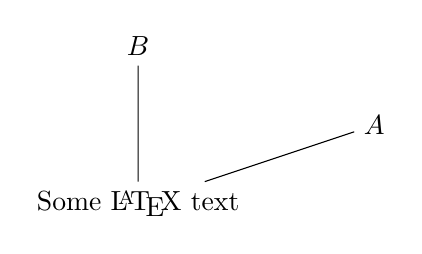
\begin{tikzpicture}
  \node (text) at (0,0) {%
    Some \LaTeX{} text};
  \node (A) at (3, 1) {\(A\)};
  \node (B) at (0, 2) {\(B\)};
  \draw (A) -- (text) -- (B);
\end{tikzpicture}
\end{example}
By default \TikZ{} attempts to position the lines between nodes in a smart way.
If you want to set them manually you can specify the exact point on a node
after a dot. The available points are, for example, \cargv{north},
\cargv{west}, \cargv{south east} and so on. You can also put a number, which
will be interpreted as an angle.
\begin{example}
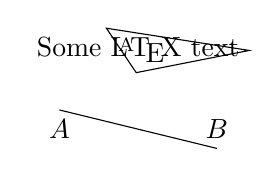
\begin{tikzpicture}
  \node (T) at (1,1) {%
    Some \LaTeX{} text};
  \node (A) at (0, 0) {\(A\)};
  \node (B) at (2, 0) {\(B\)};
  \draw (A.north) -- (B.south);
  \draw (T.0) -- (T.145)
    -- (T.265) -- cycle;
\end{tikzpicture}
\end{example}

Nodes can be also created directly while creating paths by typing \ltx{node}
after a given coordinate or a line. If they are added after a line, they will
be placed at the midpoint.
\begin{example}
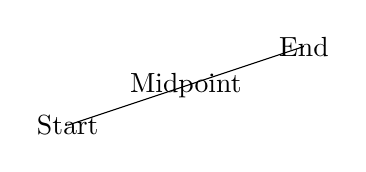
\begin{tikzpicture}
  \draw (0, 0) node {Start}
    -- node {Midpoint}
    (3, 1) node {End};
\end{tikzpicture}
\end{example}

If you want to create an empty node for the purpose of naming a specific point,
it is better to use the \csi{coordinate} command instead of a \csi{node}. This
ensures that the node is actually empty, since nodes created by \csi{node} by
default take up some space even if no content is present in them.
\begin{example}
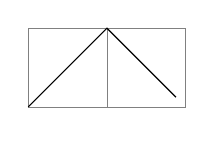
\begin{tikzpicture}
  \draw [help lines] (0, 0) grid (2, 1); % !hide
  \coordinate (A) at (0, 0);
  \coordinate (B) at (1, 1);
  \node (C) at (2, 0) {};
  \draw (A) -- (B) -- (C);
\end{tikzpicture}
\end{example}

\section{Curves and Shapes}

So far we have always used \ltx|--| to connect points, however,
this is not the only way. For example, if you wanted to only use horizontal and
vertical lines you could specify \ltx/-|/ or \ltx/|-/ (depending on preferred
order) as connection between points.
\begin{example}
\tikz{\draw (0, 0) |- (2, 1);}
\tikz{\draw (0, 0) -| (2, 1);}
\end{example}

If you want to create curved lines the simplest way is to use \ltx{to} to
connect points. By default it works the same as \ltx{--}, but it can receive
optional argument with \cargv{in} and \cargv{out} keys to define the angle of
connection.
\begin{example}[vertical_mode, examplewidth=0.8\linewidth]
\tikzset{baseline} \vspace{-0.3cm} %!hide
\tikz{\draw (0, 0) to[out=90, in=-90] (2, 0);}
\tikz{\draw (0, 0) to[out=45] (2, 0);}
\vspace{-0.5cm} %!hide
\end{example}
The \cargv{looseness} key may be used to define how much the curve is outstretched.
\begin{example}[vertical_mode, examplewidth=0.8\linewidth]
\tikzset{baseline} \vspace{-1cm} %!hide
\tikz{\draw (0, 0)
  to[out=90, in=-90, looseness=0.5] (2, 0);}
\tikz{\draw (0, 0) 
  to[out=90, in=-90, looseness=2] (2, 0);}
\vspace{-1cm} %!hide
\end{example}
Often it might be easier to specify the angles relatively using \cargv{bend
  left} and \cargv{bend right} keys. If no angle is provided they will use a
default value.
\begin{example}[vertical_mode, examplewidth=0.8\linewidth]
\tikz{\draw (0, 0) to[bend left] (2, 0);}
\tikz{\draw (0, 0) to[bend right=90] (2, 0);}
\end{example}

If you need even finer control over the curves you can use the
\ltx{.. controls ..} connection for specifying them as Bézier curve with one
or two control points.
\begin{chktexignore}  
\begin{example}[vertical_mode, examplewidth=0.8\linewidth]
\vspace{-0.5cm} %!hide
\tikz{\draw (0, 0) .. controls (1, 1) .. (2, 0);}
\tikz{\draw (0, 0) .. controls (.5, 2) and (3, 1)
  .. (2, 0);}
\end{example}
\end{chktexignore}

In addition to curves, the points may also be connected using various shapes.
For example the \ltx{grid} draws a grid between the points, while
\ltx{rectangle} draws a rectangle.
\begin{example}[vertical_mode, examplewidth=0.8\linewidth]
\tikz{\draw (0, 0) grid (2, 2);}
\tikz{\draw (0, 0) rectangle (3, 1);}
\end{example}
To specify how fine the grid is, use the \cargv{step} key.
\begin{example}[vertical_mode, examplewidth=0.8\linewidth]
\tikz{\draw (0, 0) grid[step=0.5] (2, 2);}
\tikz{\draw (0, 0) grid[step=1.5] (2, 2);}
\end{example}

Other shapes may also be drawn this way, sometimes requiring a specific syntax.
For example the \ltx{circle} interprets the left coordinate as its centre and
receives its radius via the \cargv{radius} key. You can also specify \cargv{x
  radius} and \cargv{y radius} separately, thus drawing an ellipse\footnote{The
  \cargv{ellipse} shape can also be used in the same way if the naming irks you
  \smiley.}.
\begin{example}[vertical_mode, examplewidth=0.9\linewidth]
\tikz{\draw (0, 0) circle[radius=1];}
\tikz{\draw (0, 0) circle[x radius=2, y radius=0.5];}
\end{example}
Many more shapes are available, such as \ltx{arc}, \ltx{parabola} or \ltx{sin}.
Be sure to checkout the documentation for the specifics of their use.

\section{Customising Paths and Nodes}

By default all paths are drawn using a black continuous lines. You can modify
them by passing options to the \csi{draw} command. For example, simply passing
a colour name will change the colour of the drawn line.
\begin{example}
\tikz{\draw[red]
  (0, 0) -- (1, 1);}
\tikz{\draw[blue]
  (0, 0) -- (1, 1);}
\end{example}

The thickness of a line can be controlled by passing \cargv{line width} key
(specified in points by default), or using some predefined values such as
\cargv{semithick}, \cargv{very thin} or \cargv{ultra thick}.
\begin{example}
\tikz{\draw[line width=2]
  (0, 0) -- (1, 1);}
\tikz{\draw[very thin]
  (0, 0) -- (1, 1);}
\end{example}

The endings of lines can also be customised using several different keys. For
example \cargv{line cap} allows you to change the drawn lines to have rounded
corners.
\begin{example}
\tikz{\draw[line width=10]
  (0, 0) -- (1, 1);}
\tikz{\draw[line width=10,
  line cap=round]
  (0, 0) -- (1, 1);}
\end{example}
You can also turn them into arrows by specifying \cargv{arrows} key.
\begin{example}
\tikz{\draw[arrows=->]
  (0, 0) -- (1, 1);}
\tikz{\draw[arrows=<<->]
  (0, 0) -- (1, 1);}
\end{example}

The lines don't need to be continuous either. You can specify \cargv{dash
  pattern} or use one of the predefined ones to create dashed paths.
\begin{example}
\tikz{\draw[dash pattern=
  on 4 off 1 on 2 off 1]
  (0, 0) -- (1, 1);}
\tikz{\draw[dotted]
  (0, 0) -- (1, 1);}
\end{example}

You can also adjust how the lines are connected with other lines. For example,
you can pass \cargv{line join} set to \cargv{round}, \cargv{bevel}, or
\cargv{miter}.
\begin{example}
\tikzset{every picture/.style={line width=6pt}} %!hide
\tikz{\draw[line join=round]
  (0, 0) -- (0.5, 1) -- (1, 0);}
\tikz{\draw[line join=bevel]
  (0, 0) -- (0.5, 1) -- (1, 0);}
\end{example}
If you want the line joins to be rounded you can also pass the \cargv{rounded
  corners} key with the value set to the radius of the arc.
\begin{example}
\tikz{\draw[rounded corners]
  (0, 0) -- (0.5, 1) -- (1, 0);}
\tikz{\draw[rounded corners=25]
  (0, 0) -- (0.5, 1) -- (1, 0);}
\end{example}

Now, let's turn our attention nodes. By default node's boundary is not drawn,
but you can pass \cargv{draw} and \cargv{fill}, possibly set to a colour, to
reveal it.
\begin{example}
\tikz{\node[draw] (0, 0)
  {Some Text};}
\tikz{\node[fill=red] (0, 0)
  {Some Text};}
\end{example}
As you can see all nodes are rectangles, but they can be changed to circles if
you pass the \cargv{circle} key to their options.
\begin{example}
\tikz{\node[draw, circle]
  (0, 0) {Some text};}
\end{example}

If you want to input multi line text inside nodes, you have to specify the
\cargv{align} key; without it new lines will be simply ignored. Possible values
are \cargv{left}, \cargv{center} and \cargv{right}.
\begin{example}
\tikz{\node[draw, align=left]
  (0, 0) {Some more\\ text};}
\tikz{\node[draw, align=center]
  (0, 0) {Even more \\ text};}
\end{example}

When nodes are placed along a path, their position may be adjusted using
\cargv{anchor} key. Its value is the point of node which should be anchored at
the given point in path.
\begin{example}
\tikz{\draw
  (0, 0) node[anchor=south] {A}
  -- node[anchor=north west] {B}
  (1, 1) node[anchor=135] {C};
}
\end{example}
Usually using relative commands such as \cargv{left} or \cargv{above right} for
this purpose leads to a more readable code, though they are not as powerful.
\begin{example}
\tikz{\draw
  (0, 0) node[above] {A}
  -- node[below right] {B}
  (1, 1) node[right] {C};
}
\end{example}

All of the options can be obviously freely combined, but the resulting style
specification may turn out to be long. To avoid retyping it for many nodes or
paths you can define styles. Some predefined styles already exist. For example,
the \cargv{help lines} style sets the colour of lines to grey and makes them a
bit thinner, which is useful for drawing helping grids, when drawing your own
pictures.
\begin{example}
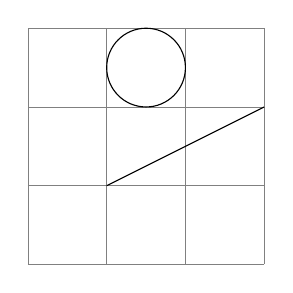
\begin{tikzpicture}
  \draw[help lines]
    (0, 0) grid (3,3);
  \draw (1, 1) -- (3,2);
  \draw (1.5, 2.5)
    circle[radius=0.5];
\end{tikzpicture}
\end{example}
To define your own style, pass key of the form
\cargv{\carg{name}/.style=\carg{options}} to the \TikZ{} environment or
command options.
\begin{example}[vertical_mode, examplewidth=0.7\linewidth]
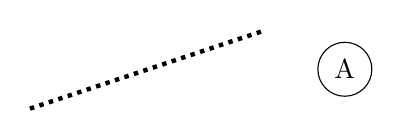
\begin{tikzpicture}[
  my line/.style={dotted, ultra thick},
  my node/.style={draw, circle},
]
  \draw[my line] (0, 0) -- (3, 1);
  \node[my node] at (4, 0.5) {A};
\end{tikzpicture}
\end{example}
If you want to set up some styles globally you can also use the \csi{tikzset}
command.
\begin{example}
\tikzset{
  red style/.style={draw=red},
}
\tikz{\draw[red style]
  (0, 0) -- (1, 1) -- (2, 0);}
\tikz{\node[red style]
  at (0, 0) {Red node};}
\end{example}
If you want to avoid specifying the style with every node or path within
\TikZ{} picture, you can also set a special styles \cargv{every node} and
\cargv{every path} to change them all at once.
\begin{example}
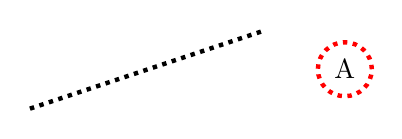
\begin{tikzpicture}[
  every path/.style={
    ultra thick, dotted},
  every node/.style={
    circle, draw=red},
]
  \draw (0, 0) -- (3, 1);
  \node at (4, 0.5) {A};
\end{tikzpicture}
\end{example}

\section{Coordinates}

So far we have always used the default centimetres for specifying coordinates,
however it is possible to use any \LaTeX{} dimension (see
\autoref{sec:dimensions} for details).
\begin{example}
\tikz{\draw (0, 0)
  -- (1in, 1pt);}
\tikz{\draw (0, 0)
  -- (1dd, 1em);}
\end{example}

It is also possible to rescale how the distances are measured by using the
\cargv{scale} key. This is useful if you find that your picture is too big or
too small after drawing it, or if there exist some intuitive coordinate system
(for example, when drawing function plots).
\begin{example}
\tikz[scale=2]{\draw
  (0, 0) -- (1, 1);}
\tikz{\draw (0, 0) -- (2, 2);}
\end{example}
You can also specify \cargv{xscale} and \cargv{yscale} separately.

When specifying scale you can use simple arithmetic operations. For example, to
change the dimensionless values to inches, you can pass \ltx{scale=1in/1cm}.
\begin{example}
\tikz[scale=1in/1cm]{\draw
  (0, 0) -- (1, 0.5);}
\tikz[scale=1em/1cm]{\draw
  (0, 0) -- (1, 0.5);}
\end{example}
Keep in mind that coordinates with dimensions will also be scaled, which may
have unintended consequences. More robust way of changing the dimensionless
values are the \cargv{x} and \cargv{y} keys.
\begin{example}
\tikz[x=1in, y=1in]{\draw
  (0, 0) -- (1, 0.5);}
\tikz[x=1em, y=10ex]{\draw
  (0, 0) -- (1, 0.5);}
\end{example}

You can actually specify three dimensional coordinates when drawing pictures.
By default, the third coordinate is interpreted as a vector pointing \(45\)
degrees to the bottom left and is a bit shorter (formally \((0, 0, 1)\) is  the
same as \((-0.385, -0.385)\)). This gives the effect of parallel (or
axonometric) projection.
\begin{example}[vertical_mode, examplewidth=0.85\linewidth]
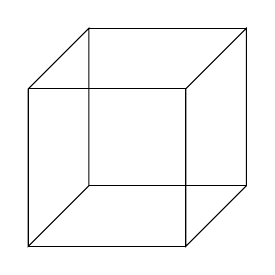
\begin{tikzpicture}[scale=2]
  \draw (0, 0, 0) -- (0, 0, 1) -- (0, 1, 1) -- 
    (0, 1, 0) -- cycle;
  \draw (1, 0, 0) -- (1, 0, 1) -- (1, 1, 1) -- 
    (1, 1, 0) -- cycle;
  \draw (0, 0, 0) -- (1, 0, 0) (0, 0, 1) -- (1, 0, 1)
    (0, 1, 1) -- (1, 1, 1) (1, 1, 0) -- (0, 1, 0);
\end{tikzpicture}
\end{example}
Its length and direction can also be changed by using \cargv{z} key.

Sometimes it may be easier to specify the path by using coordinates relative to
the previous point instead of absolute ones. To do so prepend \ltx{++} to the
coordinate, which will be interpreted as the previous specified point with the
coordinate added.
\begin{example}
\begin{tikzpicture}[scale=2]
  \draw (0, 0) -- ++(0, 1) -- 
    ++(1, 0) -- ++(0, -1) --
    cycle;
  \draw (1.5, 0) -- ++(0, 1) -- 
    ++(1, 0) -- ++(0, -1) --
    cycle;
\end{tikzpicture}
\end{example}

Scaling is not the only transformation that can be applied to points. It is
also possible to rotate, shift or apply an arbitrary linear transformation by
specifying its matrix. Check out the documentation for a detailed description.
\begin{example}
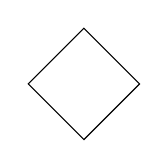
\begin{tikzpicture}[rotate=45]
  \draw (0, 0) -- (0, 1) -- 
    (1, 1) -- (1, 0) -- cycle;
\end{tikzpicture}
\end{example}
It is also possible to apply transformations to a single command.
\begin{example}
\begin{tikzpicture}
  \draw (0, 0) -- (1, 1);
  \draw[red, xshift=1cm]
    (0, 0) -- (1, 1);
\end{tikzpicture}
\end{example}
If you want to apply the same transformation to more than one command within
the same picture you can use \ei{scope} environment. It is especially useful
when your picture consists of more than one subpictures each of which is more
or less independent.
\begin{example}[vertical_mode, examplewidth=0.7\linewidth]
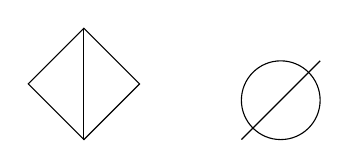
\begin{tikzpicture}
  \begin{scope}[rotate=45]
    \draw (0, 0) rectangle (1, 1);
    \draw (0, 0) -- (1, 1);
  \end{scope}
  \begin{scope}[xshift=2cm]
    \draw (0.5, 0.5) circle [radius=0.5];
    \draw (0, 0) -- (1, 1);
  \end{scope}
\end{tikzpicture}
\end{example}

When \TikZ{} pictures are positioned within text, their bottom part matches the
baseline of the text. If you want to modify it you can use \cargv{baseline} key
to set at which \(y\) coordinate should the baseline be. If no dimension is
specified it defaults to \(0\).
\begin{example}[vertical_mode, examplewidth=0.8\linewidth]
text \tikz{\draw (0, 0) circle [radius=1em];}
text \tikz[baseline]{\draw 
  (0, 0) circle [radius=1em];}
text \tikz[baseline=-0.5ex]{\draw
  (0, 0) circle [radius=1em];} text
\end{example}

\section{Reusing Pictures}

Sometimes you may wish to put the same picture in few places of a bigger
picture. While you could use commands described in
\autoref{sec:simple_commands}, this would be problematic since modifying their
placement or style is non-trivial. \TikZ{} comes with its own method of
defining smaller pictures called pics. They can be created by passing
\cargv{\carg{name}/.pic=\carg{commands}} to the \TikZ{} environment or command
and then used by invoking \csi{pic} command. An example of using it is
presented in \autoref{lst:pics}.
\begin{listing}
  \begin{example}[vertical_mode, examplewidth=0.9\linewidth]
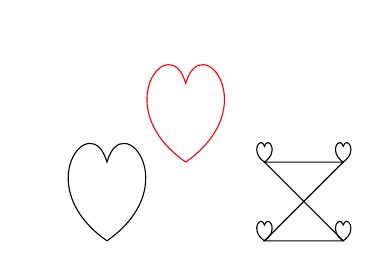
\begin{tikzpicture}[
  heart/.pic={
    \draw (0,0) .. controls (-1, 0.7) and (-0.2, 1.7) 
    .. (0, 1) .. controls  (0.2, 1.7) and (1, 0.7) 
    .. (0, 0);
  },
]
  \pic at (0, 0) {heart};
  \pic[red] at (1, 1) {heart};

  \begin{scope}[xshift=2cm, every pic/.style={scale=0.2}]
    \draw (0, 0) pic {heart} -- (1, 1) pic {heart} --
      (0, 1) pic {heart} -- (1, 0) pic {heart} -- cycle;
  \end{scope}
\end{tikzpicture}
\end{example}
  \caption{An example of using pics in \TikZ{}.}\label{lst:pics}
\end{listing}
If you find yourself repeating a lot of simple commands (for example, drawing
ticks on an axis) you may simplify your code by using \csi{foreach} command. It
repeats the drawing command for each value in a provided list, so that you can
only write repeatable code once and only modify the important parts.
\begin{example}[vertical_mode, examplewidth=0.8\linewidth]
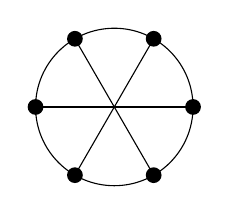
\begin{tikzpicture}
  \draw (0, 0) circle[radius=1cm];
  \foreach \i in {0, 60, 120, 180, 240, 300} {
    \draw (0, 0) -- (\i: 1);
    \fill (\i: 1) circle[radius=0.1cm];
  }
\end{tikzpicture}
\end{example}
If your values are a simple arithmetic sequence you can only provide first two
and last value, replacing the rest with triple dots.
\begin{example}[vertical_mode, examplewidth=0.8\linewidth]
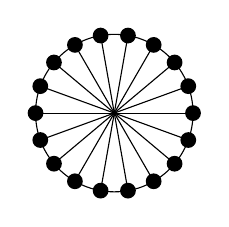
\begin{tikzpicture}
  \draw (0, 0) circle[radius=1cm];
  \foreach \i in {0, 20, ..., 340} {
    \draw (0, 0) -- (\i: 1);
    \fill (\i: 1) circle[radius=0.1cm];
  }
\end{tikzpicture}
\end{example}
You can also iterate over pairs by separating respective parts by \ltx{/}.
\begin{example}
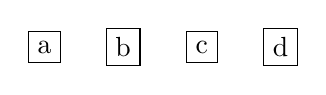
\begin{tikzpicture}
  \foreach \i/\j in {0/a,
    1/b, 2/c, 3/d} {
    \node[draw] at (\i, 0) {\j};
  }
\end{tikzpicture}
\end{example}

\section{Libraries}

\pai{pgf} and \TikZ{} do not rely on \LaTeX{}. In fact they can be used with
any \TeX{} based system or the \TeX{} itself. For this reason \TikZ{} provides
its own system of extensions that does not use \LaTeX{}'s \cs{usepackage}
command. Extensions of \TikZ{} are called libraries and can be loaded using
\csi{usetikzlibrary} command which receives a list of comma separated
libraries.

For example, if you intend to draw some geometric problems, you will often find
yourself looking for intersections of some objects. While you could calculate
their exact coordinates by hand, the \cargv{intersections} library will do it
for you. An example of using it is presented in \autoref{lst:intersections};
\begin{listing}
  \begin{example}[vertical_mode, examplewidth=0.8\linewidth]
%!showbegin !hide
% In preamble
\usetikzlibrary{intersections}
% ...
%!showend !hide

\begin{tikzpicture}
  \draw[name path=O] (0, 0) circle [radius=1];
  \draw[name path=L] (-2, -1.5) -- (3, 1);

  \fill[red, name intersections={of=O and L}]
    (intersection-1) circle[radius=2pt]
    (intersection-2) circle[radius=2pt];
\end{tikzpicture}
\end{example}
  \caption{An example of using \cargv{intersections}
    library.}\label{lst:intersections}
\end{listing}

Other libraries extend the number of available shapes. For example, the
\cargv{arrows.meta} library defines a lot of additional arrow tips if you do
not like the classical one. Some of the available ones are presented in
\autoref{lst:arrows.meta}.
\begin{listing}
  \begin{example}[vertical_mode, examplewidth=0.8\linewidth]
%!showbegin !hide
% In preamble
\usetikzlibrary{arrows.meta}
% ...
%!showend !hide

\tikzset{every path/.style={ultra thick}} %!hide2
\tikz{\draw[->] (0, 0) -- (1, 1);}
\tikz{\draw[-{Circle}] (0, 0) -- (1, 1);}
\tikz{\draw[-{Stealth}] (0, 0) -- (1, 1);}
\tikz{\draw[-{Stealth[round]}] (0, 0) -- (1, 1);}
\tikz{\draw[-{Diamond[open]}] (0, 0) -- (1, 1);}
\end{example}
  \caption{Some of the arrow tips defined by \cargv{arrows.meta}
    library.}\label{lst:arrows.meta}
\end{listing}
Oftentimes you may want to perform additional computations on existing
coordinates. The \cargv{calc} library allows you to do so by enclosing them
within \verb|$| symbols.
\begin{example}[vertical_mode, examplewidth=0.8\linewidth]
%!showbegin !hide
% In preamble
\usetikzlibrary{calc}
% ...
%!showend !hide

\begin{tikzpicture}
  \coordinate (A) at (1, -1);
  \coordinate (B) at (0, 1);
  \draw[red, ->] (0, 0) -- node[above] {\(A\)} (A);
  \draw[blue, ->] (0, 0) -- node[left] {\(B\)} (B);
  \draw[green, ->] (0, 0) -- 
      node[below right] {\(A+2B\)} ($(A)+2*(B)$);
\end{tikzpicture}
\end{example}

If you have a lot of \TikZ{} code in your document you may notice that
compiling your document takes up much more time than initially. This is because
\TikZ{} redraws each picture with every \LaTeX{} pass. If this starts getting
annoying you can cache your images to external files and reuse them on
subsequent runs. To do this simply put the following code in your preamble.
\begin{minted}{latex}
\usetikzlibrary{external}
\tikzexternalize
\end{minted}
This method has some limitations, but should be sufficient for most uses. Read
up on it in documentation if problems occur.

There are many more libraries, most of which are described in the \pai*{pgf}
package documentation. Check it out if you haven't found solution to your
problem here.

% The Not So Short Introduction to LaTeX
%
% Copyright (C) 1995--2022 Tobias Oetiker, Marcin Serwin, Hubert Partl,
% Irene Hyna, Elisabeth Schlegl and Contributors.
%
% This document is free software: you can redistribute it and/or modify it
% under the terms of the GNU General Public License as published by the Free
% Software Foundation, either version 3 of the License, or (at your option) any
% later version.
%
% This document is distributed in the hope that it will be useful, but WITHOUT
% ANY WARRANTY; without even the implied warranty of MERCHANTABILITY or FITNESS
% FOR A PARTICULAR PURPOSE.  See the GNU General Public License for more
% details.
%
% You should have received a copy of the GNU General Public License along with
% this document.  If not, see <https://www.gnu.org/licenses/>.

% !TEX root = ./lshort.tex
%%%%%%%%%%%%%%%%%%%%%%%%%%%%%%%%%%%%%%%%%%%%%%%%%%%%%%%%%%%%%%%%%
% Contents: Customising LaTeX output
% $Id$
%%%%%%%%%%%%%%%%%%%%%%%%%%%%%%%%%%%%%%%%%%%%%%%%%%%%%%%%%%%%%%%%%
\chapter{Customising \LaTeX}\label{chap:custom}

\begin{intro}
  Documents produced with the commands you have learned up to this
  point will look acceptable to a large audience. While they are not
  fancy-looking, they obey all the established rules of good
  typesetting, which will make them easy to read and pleasant to look at.

  However, there are situations where \LaTeX{} does not provide a
  command or environment that matches your needs, or the output
  produced by some existing command may not meet your requirements.

  In this chapter, I will try to give some hints on
  how to teach \LaTeX{} new tricks and how to make it produce output
  that looks different from what is provided by default.
\end{intro}

\section{New Commands, Environments and Packages}

At the beginning of this book we have mentioned that \LaTeX{} allows us to
write documents using logical markup, with commands like \csi{emph} or \csi{section}. There
may be however situations where \LaTeX{} does not provide an appropriate command for the content you want write about.
You may have noticed that all the
commands I introduce in this book are typeset in a box, and that they show up
in the index at the end of the book. There is no \LaTeX{} markup to format example code or commands, but \LaTeX{} allows me to define my own commands for this purpose. Thus I
can write:

\begin{example}
\begin{lscommand}
  \csi{dum}
\end{lscommand}
\end{example}

In this example, I am using both a new environment called
\ei{lscommand}, which is responsible for drawing the box around the
command, and a new command named \csi{csi}, which typesets the command
name and makes a corresponding entry in the index. Check
this out by looking up the \csi{dum} command in the index at the back
of this book, where you'll find an entry for \csi{dum}, pointing to
every page where I mentioned the \csi{dum} command.

If I ever decide that I do not like having the commands typeset in
a box any more, I can simply change the definition of the
\ei{lscommand} environment to create a new look. This is much
easier than going through the whole document to hunt down all the
places where I have used some generic \LaTeX{} commands to draw a
box around some word.

\subsection{New Commands}\label{sec:new_commands}

You have already learned some basic command creation in
\autoref{sec:simple_commands}. The main command is the
\begin{lscommand}
  \csi{NewDocumentCommand}[name:M, argspec:m, definition:m]
\end{lscommand}
It requires three arguments: the \carg{name} of the command you want to create,
the \carg{argspec} (argument specification) and the \emph{definition} of the
command.

The \carg{argspec} argument specifies the number and types of arguments the
command receives. The two most important types are \cargv{m}, for
\emph{mandatory} and \cargv{o} for \emph{optional}. To create a command that
takes two optional arguments, then two mandatory, then again one optional and
finally three mandatory you would write \cargv{oommommm}. If the \carg{argspec}
argument is empty then the command will take no arguments, as you have already
seen.

This example defines a new command called \csi{tnss}. This is
short for \enquote{The Not So Short Introduction to \LaTeX}. Such a command
could come in handy if you had to write the title of this book over
and over again.

\begin{example}
\NewDocumentCommand{\tnss}{}{%
  The not so Short Introduction
    to \LaTeX}
This is \enquote{\tnss} \ldots{}
\enquote{\tnss}
\end{example}

The next example illustrates how to define a new command that takes two
arguments. In order to refer to the received arguments you use
\mintinline{latex}|#1| for the first argument, \mintinline{latex}|#2| for the
second, and so on.

\begin{example}
\NewDocumentCommand{\txsit}{mm}
 {This is the \emph{#1}
  #2 Introduction to \LaTeX}

% in the document body:
\txsit{not so}{short}

\txsit{very}{long}
\end{example}

If your command accepts an optional argument but the user does not supply one,
a special marker \cargv{-NoValue-} will be inserted instead.
\begin{example}
\NewDocumentCommand{\txsit}{om}
{This is the \emph{#1}
  #2 Introduction to \LaTeX}

% in the document body:
\txsit{definitive}

\txsit[very]{long}
\end{example}
In order to test whether the user supplied a value, use
\begin{lscommand}
  \csi{IfValueTF}[argument:m, value version:m, no value version:m]
\end{lscommand}
macro.
\begin{example}
\NewDocumentCommand{\MyCommand}{o}{
  \IfValueTF {#1} {
    Optional argument: #1.
  } {
    No optional argument given.
  }%
}

\MyCommand\\
\MyCommand[hello]
\end{example}

There are two variations of it: \csi{IfValueT} and \csi{IfValueF} which may
be used if you only need output for one of the branches. The example with
\cargv{-NoValue-} in the output could be fixed by writing
\begin{example}
\NewDocumentCommand{\txsit}{om}
{This is the
  \IfValueT{#1}{\emph{#1} }%
  #2 Introduction to \LaTeX}

% in the document body:
\txsit{definitive}

\txsit[very]{long}
\end{example}
The commands \csi{IfNoValueTF}, \csi{IfNoValueT} and \csi{IfNoValueF}
work exactly the same, but the value\slash{}no-value branches are swapped.

Often you will want to use optional arguments when present but use some default
values when the user does not provide them. This could be achieved by
\csi{IfValueTF}, but with the \cargv{O} argument a default value can be set directly.
It works like \cargv{o} but allows to set a default
if no value is supplied. Write

\begin{example}
\NewDocumentCommand{\txsit}{O{not so}m}
{This is the \emph{#1}
  #2 Introduction to \LaTeX}

% in the document body:
\txsit{definitive}

\txsit[very]{long}
\end{example}

Another useful argument specification is \cargv{s}, short for star. This
argument allows to provide different definitions based on whether the
starred or non-starred version of command was issued by the user. It uses
\csi{IfBooleanTF} command (and its variations\csih{IfBooleanT}\csih{IfBooleanF})
that works analogously to the \csi{IfValueTF} command.

\begin{chktexignore}
  \begin{example}
\NewDocumentCommand{\txsit}{sO{not so}m}
{This is the \emph{#2}
  #3 Introduction to \LaTeX%
  \IfBooleanT{#1}{%
    : Superstar Edition%
  }%
}

% in the document body:
\txsit{long}\\
\txsit*{long}
\end{example}
\end{chktexignore}

These are just the most common argument specifications. For a full description,
take a look at the~\cite{usrguide3}.

As we have discussed in \autoref{sec:simple_commands}, \LaTeX{} will not allow
you to create a new command that would overwrite an existing one, you can do so
using \csi{RenewDocumentCommand}. It uses the same argument specification
syntax as the \csi{NewDocumentCommand} command.

In some cases you might want to use the \csi{ProvideDocumentCommand} command.
It works like \csi{NewDocumentCommand}, but if the command is already defined,
\LaTeX{} will silently ignore the new definition. Yet another variant is the
\csi{DeclareDocumentCommand}. It always creates the given command, overwriting
old definition if it exists.

\subsection{New Environments}
The \csi{NewDocumentEnvironment} command lets you create your own environments. It has the
following syntax:

\begin{lscommand}
  \small
  \csi{NewDocumentEnvironment}[name:m, argspec:m, at begin:m, at end:m]
\end{lscommand}
The \carg{argspec} argument is the same as in the
\csi{NewDocumentCommand} command. The contents of \carg{at begin} and \carg{at
  end} arguments will be inserted respectively when the commands
\csi{begin}[name: m] and \csi{end}[name: m] is encountered. The example
presented in \autoref{lst:kingenv} illustrates the usage of this command.
\begin{listing}
  \begin{example}
\NewDocumentEnvironment{king}{}{%
  \emph{Listen! For the
    king made a statement:}%
  \\[1em]%
} {%
  \\[1em]%
  \emph{This concludes
    the king's statement.}%
}

\begin{king}
My humble subjects \ldots
\end{king}
\end{example}
  \caption{An example of using \csi{NewDocumentEnvironment}
    command.}\label{lst:kingenv}
\end{listing}

Note that when environment argument are read, they are read \emph{after} the
\csi{begin}[name: m] command. This may be especially counter intuitive when we
consider the \cargv{s} specification. \autoref{lst:kingsenv} illustrates this.
\begin{listing}
  \begin{example}
\NewDocumentEnvironment{king}{s}{%
  \IfBooleanTF{#1}{
    \begin{center}
      \emph{Thus spoke Charles I:}
      \\[1em]%
    \end{center}%
  } {
    \emph{Listen! For the
      king made a statement:}%
      \\[1em]%
  }%
} {%
  \\[1em]%
  \emph{This concludes
    the king's statement.}%
}

\begin{king}*
My humble subjects \ldots
\end{king}
\end{example}
  \caption{An example of using the \cargv{s} specifier when defining a new
    environment.}\label{lst:kingsenv}
\end{listing}
If you want to create a starred version of an environment (similarly to some
\hologo{AmSLaTeX} environments) you have to define it separately.
\begin{minted}{latex}
\NewDocumentEnvironment{king}{moo} { ... } { ... }
\NewDocumentEnvironment{king*}{moo} { ... } { ... }
\end{minted}
Obviously you can use the same internal commands to define them, for example
renaming the previous implementation to \cargv{kinginternal} making the
\cargv{king} and \cargv{king*} a thin wrapper around it.

The \csi{NewDocumentEnvironment} also introduces a special argument
specification: \cargv{+b}, short for body.\footnote{The \cargv{+} indicates
  that it may contain multiple paragraphs.} It is only allowed as the last
argument in the \carg{argspec}. It allows you to receive the body of the
environment as an argument.
\begin{example}
\NewDocumentEnvironment{twice}{+b} {%
  First time:\\ #1

  Second time:\\ #1
} {}

\begin{twice}
This will be printed twice!
\end{twice}
\end{example}
While this makes one of the \carg{at begin}, \carg{at end} arguments redundant,
they are still required. (In the example above we provided an empty \carg{at
  end}.)

Do not overuse \cargv{+b} as this will both make the environments subject to
some limitations (e.g.\ \csi{verb} will not be allowed inside) and slow down the
typesetting.

Similarly to the \csi{NewDocumentCommand} \LaTeX{} makes sure that you do not
define an environment that already exists. If you ever want to change an
existing environment, use the \csi{RenewDocumentEnvironment} command. Its
arguments are the same as the \csi{NewDocumentEnvironment} command.

\subsection{Copying commands}\label{sec:copyingcommands}

When redefining commands you may want to use the original version of the
command. Your initial code may look like this
\begin{minted}{latex}
\RenewDocumentCommand{\emph}{m}{%
  \emph{#1}~(\enquote{#1} is emphasised)%
}
\end{minted}
but when you try to compile the document you will receive the error
\begin{verbatim}
! TeX capacity exceeded, sorry [input stack size=5000].
\end{verbatim}

To understand why this happens it is instructive to consider how \TeX{} expands
the defined commands. The above \csi{RenewDocumentCommand} tells the \TeX{}
engine that whenever \csi{emph}[foo:vm] is seen it must replace it with
\mintinline{latex}|\emph{foo}~(\enquote{foo} is emphasised)|. You may already see the
problem here. In the next stage it will again replace the \csi{emph}[foo:vm]
yielding
\begin{minted}[breaklines]{latex}
\emph{foo}~(\enquote{foo} is emphasised)~(\enquote{foo} is emphasised)
\end{minted}
This process will never end and at some point \TeX{}
simply gives up.

Note that
\begin{minted}{latex}
\NewDocumentCommand{\oldemph}{m}{\emph{#1}}
\RenewDocumentCommand{\emph}{m}{%
  \oldemph{#1}~(\enquote{#1} is emphasised)%
}
\end{minted}
will suffer the same fate since \mintinline{latex}|\oldemph{...}| %chktex 11 
will  be replaced by \TeX{} with \mintinline{latex}|\emph{...}| and %chktex 11
the  cycle repeats.

In order to avoid this problem a special command exists
\begin{lscommand}
  \csi{NewCommandCopy}[name:M, command:M]
\end{lscommand}
It makes the \carg{name} the exact copy of the \carg{command}. The following example shows how this works
\begin{example}[examplewidth=0.35\linewidth]
\NewDocumentCommand{\foo}{}{Batman!}

\NewDocumentCommand{\newfoo}{}{\foo}
\NewCommandCopy{\copiedfoo}{\foo}

\RenewDocumentCommand{\foo}{}{Na Na Na}

\foo{} \newfoo{} \copiedfoo{}
\end{example}

This is precisely the behaviour we need in order to redefine the \csi{emph}
command as we have tried to do earlier.
\begin{example}[examplewidth=0.35\linewidth]
\NewCommandCopy{\oldemph}{\emph}
\RenewDocumentCommand{\emph}{m}{%
  \oldemph{#1}~(\enquote{#1}
  is emphasised)%
}

And here it \emph{comes}.
\end{example}

\subsection{Command-line \LaTeX}

If you work on a Unix-like OS, you might be using Makefiles to build your
\LaTeX{} projects. In that connection it might be interesting to produce
different versions of the same document by calling \LaTeX{} with command-line
parameters. If you add the following structure to your document:

\begin{minted}{latex}
\IfBooleanTF{\blackandwhite} {
  % "black and white" mode; do something...
} {
  % "color" mode; do something different...
}
\end{minted}

Now compile document like this:
\begin{verbatim}
xelatex '\NewCommandCopy{\blackandwhite}{\BooleanTrue}
    \input{test.tex}'
\end{verbatim}
First the command \verb|\blackandwhite| is defined as the \csi{BooleanTrue} macro which
holds a special value used in \csi{IfBooleanTF} checks. Then the actual file is
read with input. By setting \verb|\blackandwhite| to \csi{BooleanFalse} the
colour version of the document would be produced.

\subsection{Your Own Package}

If you define a lot of new environments and commands, the preamble of
your document will get quite long. In this situation, it is a good
idea to create a \LaTeX{} package containing all your command and
environment definitions. Use the \csi{usepackage}
command to make the package available in your document.

\begin{listing}
  \begin{lined}{\textwidth}
    \begin{minted}{latex}
\ProvidesExplPackage{demopack}{2022-05-05}{0.1}{%
  Package by Tobias Oetiker
}

\NewDocumentCommand{\tnss}{} {
  The~not~so~Short~Introduction~to~\LaTeX
}
\NewDocumentCommand{\txsit}{O{not~so}} {
  The~\emph{#1}~Short~Introduction~to~\LaTeX
}

\NewDocumentEnvironment{king}{} {
  \begin{quote}
} {
  \end{quote}
}
\end{minted}
  \end{lined}
  \caption{Example Package.}\label{package}
\end{listing}

Writing a package basically consists of copying the contents of your document
preamble (with minor adjustments) into a separate file with a name ending in
\texttt{.sty}. There is one special command,
\begin{lscommand}
  \csi{ProvidesExplPackage}[name:m, date:m, version:m, description:m]
\end{lscommand}
for use at the very beginning of your package file. This command tells the
\LaTeX{} to process the  file in \emph{expl mode}. The most visible effect of
this is that all whitespace is ignored. You may have noticed that in many of
the examples above we had to end most lines with \ai{\%} to get correct spacing
in the output. In \emph{expl mode}, spaces have to be added explicitly if
needed at all. They are usually quite rare when writing a package. To insert
spaces, use the \ai{\~} character, which normally denotes non-breaking
space.\footnote{If you want to insert non-breaking space in \emph{expl mode},
  use \csi{nobreakspace}.} Paragraphs can be started with the \csi{par} command.

The arguments are used to provide information about package in the log file. If
you use this package and look at the log file you will find
\begin{verbatim}
Package: demopack 2022-05-05 v0.1 Package by Tobias Oetiker
\end{verbatim}
in the \eei{.log} file.

\csi{ProvidesExplPackage} will also issue a sensible error message when you try
to include a package twice. \autoref{package} shows a small example package
that contains the commands defined in the examples above.

\section{Fonts and Sizes}\label{sec:fontsize}

\subsection{Font Changing Commands}\index{font}\index{font size}

\LaTeX{} fonts are influenced by four parameters
\begin{description}
  \item[family] The collection of fonts. For example, \enquote*{Latin Modern
      Roman} or \enquote*{Source Code Pro}.
  \item[series] The weight of the font. For example, \enquote*{bold} or
    \enquote*{medium}.
  \item[shape] The shape of glyphs within a font family. For example,
    \enquote*{small caps} or \enquote*{italics}.
  \item[size] The size of the glyphs. For example, \enquote*{\qty{10}{pt}} or
    \enquote*{\qty{12}{pt}}.
\end{description}
\LaTeX{} automatically chooses the appropriate font family, series, shape and
size based on the logical structure of the document (sections, footnotes,
emphasis, \ldots). It is possible however to instruct \LaTeX{} manually which
font to use. It is important to note that not every combination of
family\slash{}series\slash{}shape exists as an actual font. \LaTeX{} will
complain if you try for something that does not exist.

\LaTeX{} predefines three font families to use throughout the document: the
upright or roman family accessible via \csi{textrm}, the \textsf{sans serif
  family} accessible via \csi{textsf} and monospace or typewriter family
accessible via \csi{texttt}.
\begin{example}
\textrm{Roman is the default
  in articles.} \\
\textsf{Sans serif is used in
  presentations.} \\
\texttt{Monospace is used in
  verbatim code blocks.}
\end{example}

There are only two predefined \LaTeX{} series: medium (\csi{textmd}) and bold
(\csi{textbf}).
\begin{example}
\textmd{The default.} \\
\textbf{Bold font.}
\end{example}

Shapes are a bit more complicated. The three basic shapes are: italics
(\csi{textit}), oblique or slanted\footnote{Oblique shape differs from the
  italics in that italic shape uses different glyphs while oblique shape
  uses the same glyphs but slanted. The difference is really obvious
  \fontshape{ui}\selectfont when you look at the unslanted italic font.}
(\csi{textsl}) and small capitals (\csi{textsc}).
\begin{example}
\textit{Italic shape.} \\
\textsl{Slanted shape.} \\
\textsc{Small Capitals.}
\end{example}
However there are two additional shapes that are not provided by default
\LaTeX{} fonts: swash (\csi{textsw}), for decorative fonts and spaced caps and
small caps (\csi{textssc}). These are rarely used but may come in handy when
using custom fonts as described in \autoref{sec:fontspec}.
\begin{example}
\setmainfont{EB Garamond} %!hide
Question vs. \textsw{Question}
\end{example}
In addition two virtual shapes are provided: upright (\csi{textup}) and
upper-lowercase (\csi{textulc}). These are not actually shapes but utility
commands. The former one switches back to upright font while the latter
disables small capitals. The command \csi{textnormal} is just the combination
of the two.
\begin{example}
\textsl{\textsc{Back to
  \textup{upright.}}} \\
\textsl{\textsc{Back to
  \textulc{lowercase.}}} \\
\textsl{\textsc{Back to
  \textnormal{normal.}}}
\end{example}

All of the commands described above also exist in their switch version. Instead
of receiving the text via argument, they change the font permanently until it is
changed again. For example, the switch version of \csi{textit} and \csi{textrm}
are \csi{itshape} and \csi{rmfamily}, respectively. While the argument versions
are useful for defining commands, switch versions are especially useful when
defining your own environments.
\begin{example}
Only \textit{argument} is
affected. After \itshape
everything is in italics
until \upshape is encountered.
\end{example}
Both argument and switch versions of the described commands are presented in
\autoref{tbl:fonts}.
\begin{table}
  \caption{Default font changing commands of \LaTeX.}\label{tbl:fonts}
  \begin{tabular}{@{}lll@{}}
    \toprule
    Argument Command         & Switch           & Example                      \\
    \midrule
    \csi{textrm}[text:m]     & \csi{rmfamily}   & \textrm{\wi{roman}}          \\
    \csi{textsf}[text:m]     & \csi{sffamily}   & \textsf{\wi{sans serif}}     \\
    \csi{texttt}[text:m]     & \csi{ttfamily}   & \texttt{typewriter}          \\[6pt]
    \csi{textmd}[text:m]     & \csi{mdseries}   & \textmd{medium}              \\
    \csi{textbf}[text:m]     & \csi{bfseries}   & \textbf{\wi{bold face}}      \\[6pt]
    \csi{textup}[text:m]     & \csi{upshape}    & \textup{\wi{upright}}        \\
    \csi{textit}[text:m]     & \csi{itshape}    & \textit{\wi{italic}}         \\
    \csi{textsl}[text:m]     & \csi{slshape}    & \textsl{\wi{slanted}}        \\
    \csi{textsc}[text:m]     & \csi{scshape}    & \textsc{\wi{Small Caps}}     \\
    \csi{textsw}[text:m]     & \csi{swshape}    & \textsw{\wi{Queen of Swash}} \\[6pt]
    \csi{textnormal}[text:m] & \csi{normalfont} & \textnormal{document} font   \\
    \bottomrule
  \end{tabular}
\end{table}

When working with switch versions of fonts that are slanted right it is
important to remember about \wi{italic correction}. This is a small space after
the end of right slanting text that is sometimes necessary to avoid overlapping
letters. It is inserted using \csi{/} command.
\begin{chktexignore}  
\begin{example}
Without: {\itshape oof}bar \\
With: {\itshape oof\/}bar
\end{example}
\end{chktexignore}
The italic correction is handled automatically by the argument versions of the
commands.

In contrast to the previous font changing commands, the size of font can only
be controlled via switch versions. \LaTeX{} predefines some switches for
changing font size, see \autoref{sizes} and \autoref{tab:pointsizes} for their
description.
\begin{table}
  \caption{Commands changing font size.}\label{sizes}\index{font size}
  \begin{tabular}{@{}ll@{\qquad}ll@{}}
    \toprule
    Command                     & Size                             &
    Command                     & Size                               \\
    \midrule
    \csi{tiny}                  & \tiny tiny                       &
    \csi{Large}                 & \Large larger                      \\
    \csi{scriptsize}            & \scriptsize very small           &
    \csi{LARGE}                 & \LARGE very large                  \\
    \csi{footnotesize}          & \footnotesize  quite small       &
    \multirow{2}{*}{\csi{huge}} & \multirow{2}{*}{\huge huge}        \\
    \csi{small}                 & \small small                     &
                                &                                    \\
    \csi{normalsize}            & \normalsize  normal              &
    \multirow{2}{*}{\csi{Huge}} & \multirow{2.2}{*}{\Huge largest}   \\
    \csi{large}                 & \large large                     &
                                &                                    \\
    \bottomrule
  \end{tabular}
\end{table}

\begin{table}
  \caption[Absolute point sizes in standard classes.]{Absolute point sizes in
    standard classes depending on the class option. The default class option is
    \cargv{10pt}.}\label{tab:pointsizes}\label{tab:sizes}
  \sisetup{table-format=2.2}
  \begin{tabular}{@{}lSSS@{}}
    \toprule
                       & \multicolumn{3}{c}{Size (\unit{pt})}                                   \\
    \cmidrule(l){2-4}
    Command            & {\cargv{10pt}}                       & {\cargv{11pt}} & {\cargv{12pt}} \\
    \midrule
    \csi{tiny}         & 5                                    & 6              & 6              \\
    \csi{scriptsize}   & 7                                    & 8              & 8              \\
    \csi{footnotesize} & 8                                    & 9              & 10             \\
    \csi{small}        & 9                                    & 10             & 10.95          \\
    \csi{normalsize}   & 10                                   & 10.95          & 12             \\
    \csi{large}        & 12                                   & 12             & 14.4           \\
    \csi{Large}        & 14.4                                 & 14.4           & 17.28          \\
    \csi{LARGE}        & 17.28                                & 17.28          & 20.74          \\
    \csi{huge}         & 20.74                                & 20.74          & 24.88          \\
    \csi{Huge}         & 24.88                                & 24.88          & 24.88          \\
    \bottomrule
  \end{tabular}
\end{table}

When using these commands it is important to remember that the
line spacing is only updated after the paragraph ends. To avoid putting empty
lines before the closing curly brace you may use the \csi{par} command.
\begin{example}
{\Large Here the line spacing
  is not updated. A bit tight!}

{\Large Much better! I can
  breathe freely again!\par}
\end{example}

An arbitrary font size can be specified using the
\begin{lscommand}
  \csi{fontsize}[size: m, line skip: m]\csi{selectfont}
\end{lscommand}
command combo. The \carg{line skip} determines the height of the text line and
should be usually around \(1.2\) times larger than the \carg{size}.
\begin{example}[vertical_mode, examplewidth=0.7\linewidth]
\fontsize{2cm}{2.4cm}\selectfont A big one!
\end{example}

Fun fact: \LaTeX{} default font is a bit unusual in that it looks slightly
different depending on its size. The difference is presented in the table below
where the text written using different sizes was rescaled to the same height.
\begin{center}
  \begin{tabular}{@{}lll@{}}
    \toprule
    \csi{tiny}                           &
    \csi{normalsize}                     &
    \csi{Huge}                             \\
    \midrule
    \resizebox{!}{2em}{\tiny Text}       &
    \resizebox{!}{2em}{\normalsize Text} &
    \resizebox{!}{2em}{\Huge Text}         \\
    \bottomrule
  \end{tabular}
\end{center}

In math mode the font changing commands typeset normal text. If you want to
switch to another font for math typesetting you need another special set of
commands presented in \autoref{mathfonts}.
\begin{example}
\(
  \textnormal{Normal text }
  \mathbf{math mode \frac{1}{2}}
\)
\end{example}

\begin{table}
  \caption{Math Fonts.}\label{mathfonts}
  \begin{tabular}{@{}lll@{}}
    \toprule
    Command                   & Example                  & Comment                \\
    \midrule
    \csi{mathrm}[text: m]     & $\mathrm{ABCabc123}$     &                        \\
    \csi{mathbf}[text: m]     & $\mathbf{ABCabc123}$     &                        \\
    \csi{mathsf}[text: m]     & $\mathsf{ABCabc123}$     &                        \\
    \csi{mathtt}[text: m]     & $\mathtt{ABCabc123}$     &                        \\
    \csi{mathit}[text: m]     & $\mathit{ABCabc123}$     &                        \\
    \csi{mathcal}[text: m]    & $\mathcal{ABC}$          & Only uppercase letters \\
    \csi{mathnormal}[text: m] & $\mathnormal{ABCabc123}$ & Old style numerals     \\
    \bottomrule
  \end{tabular}
\end{table}

If you need to access even more font variants and shapes\footnote{For example
  the aforementioned \fontshape{ui}\selectfont upright italic shape.} check out
\citetitle{fntguide}~\cite{fntguide}.

\subsection{Danger, Will Robinson, Danger}

Note! Using explicit font setting commands defies the the basic idea of
\LaTeX{} described in \autoref{sec:logical_structure}, which is to separate the
logical and visual markup. The fonts should get switched automatically
according to the requirements of the context. A simple rule of thumb: If you
use the same font changing command in several places in order to typeset a
special kind of information, you should use \csi{NewDocumentCommand} to define
a \enquote{logical wrapper command} for the font changing command.

\begin{example}
\NewDocumentCommand{\oops}{m}{%
 \textbf{#1}}
Do not \oops{enter} this room,
it's occupied by \oops{machines}
of unknown origin and purpose.
\end{example}

This approach has the advantage that you can decide at some later
stage that you want to use a visual representation of danger other
than \csi{textbf}, without having to wade through your document,
identifying all the occurrences of \csi{textbf} and then figuring out
for each one whether it was used for pointing out danger or for some other
reason.

\subsection{Advice}

To conclude this journey into the land of fonts and font sizes,
here is a little word of advice:\nopagebreak

\begin{quote}
  \underline{\textbf{Reme\(\mathfrak{mber}\)\Huge!}} \textit{The}
  \textsf{M\textbf{\LARGE O} \(\mathcal{R}\)\textsl{E}} fonts \Huge you
  \tiny use \footnotesize \textbf{in} a \small \texttt{document},
  \large \textit{the} \normalsize more \textsc{readable} and
  \textsl{\textsf{beautiful} it bec\large o\Large m\LARGE e\huge s}.
\end{quote}

\section{Custom Fonts with \pai{fontspec}}\label{sec:fontspec}

In the following examples we use Adobe Source fonts~\cites{sourceserif,
  sourcesans, sourcecodepro}. These fonts are included with \TeX{}Live \LaTeX{}
distributions and should be available in the directory
\begin{code}
  \nolinkurl{.../texmf-dist/fonts/opentype/adobe}
\end{code}
where the \cargv{...} denotes the path \TeX{}Live was installed to.
\hologo{LuaTeX} checks this directory automatically, so it should work fine,
but if you are using \hologo{XeTeX} you must first install these fonts in your
system. You can also download and install them manually from the links provided
in the bibliography. Alternatively swap out their respective names with some other
fonts installed in your system.

Many free OpenType fonts are available at \url{https://fontlibrary.org/}.

\subsection{Main Document Fonts}

If you are not pleased with the default Latin Modern font, you can change it to
any font installed in your system using the \pai*{fontspec} package. It provides
three main commands for changing document fonts:
\begin{lscommand}
  \csi{setmainfont}[options: o, font: m] \\
  \csi{setsansfont}[options: o, font: m] \\
  \csi{setmonofont}[options: o, font: m]
\end{lscommand}
This commands change, respectively, the main font of the document, \textsf{the
  sans serif font used in the document} and \texttt{the monospace font in the
  document}.
\begin{example}
Normal text.
  \emph{Emphasised.} \\
\textsf{Sans serif text.
  \emph{Emphasised}.} \\
\texttt{Monospace text.
  \emph{Emphasised}.} \\

\setmainfont{Source Serif Pro}
\setsansfont{Source Sans Pro}
\setmonofont{Source Code Pro}
Normal text.
  \emph{Emphasised.} \\
\textsf{Sans serif text.
  \emph{Emphasised}.} \\
\texttt{Monospace text.
  \emph{Emphasised}.}
\end{example}
Note that it is best to put these commands in the preamble of your document,
because some fonts are frozen when the body starts.

The optional \carg{options} argument accepts key value lists that allow to
customise the font features. For example, many fonts contain the, so called,
old style numerals that are not used by default. You can pass
\cargv{Number=OldStyle} if you want to use them in your document.
\begin{example}
\setmainfont{Source Serif Pro}
0123456789

\setmainfont[
  Numbers=OldStyle,
]{Source Serif Pro}
0123456789
\end{example}

Some fonts also provide special glyphs for a given language. For example the
Latin Modern Font provides a special
\enquote{\setmainfont[Language=Polish]{Latin Modern Roman}fk} ligature for the
Polish language. You can set the \cargv{Language} key to a given language to
enable these features.
\begin{example}
agrafka

\setmainfont[
  Language=Polish,
]{Latin Modern Roman}
agrafka
\end{example}
The \pai{polyglossia} package activates these features automatically so you
don't have to worry about them if you use it.

If your font supports it you may wish to enable automatic fractions insertion
with \cargv{Fractions=On} key.
\begin{example}
1/2 3/4 123/456

\setmainfont[
  Fractions=On,
]{Latin Modern Roman}
1/2 3/4 123/456

\setmainfont[
  Fractions=On,
]{Source Serif Pro}
1/2 3/4 123/456
\end{example}

The OpenType font format defines a lot of more font features, that may or may not
be supported by your font of choice. Consult with the \pai*{fontspec} package
documentation for a comprehensive description and examples.

\subsection{Specifying Fonts via Filenames}

If you do not want to install fonts in your system or you are working on a
collaborative project where not everybody has specific fonts installed, you can
specify the fonts directly via their filenames. In this case you must specify
font variations manually. Because the filenames are usually very similar, it is
possible to enter them using \cargv{*} patterns, where \cargv{*} is replaced by
the main name defined. Extension may also be passed via the \cargv{Extension}
key to avoid repetition. See \autoref{lst:fontloading} for a comparison of font
loading techniques. If the font files are not present in the same directory as
the document you may have to specify it directly using the \cargv{Path} key.
\begin{listing}
  \begin{example}[vertical_mode, examplewidth=0.8\linewidth]
\setmainfont{Source Serif Pro}
Normal text. \textit{Italics.} \textbf{Bold.}
\textit{\textbf{Bold italics.}} \\

\setmainfont{SourceSerifPro-Regular.otf}
Normal text. \textit{Italics.} \textbf{Bold.}
\textit{\textbf{Bold italics.}} \\
 
\setmainfont[
  ItalicFont=SourceSerifPro-RegularIt.otf,
  BoldFont=SourceSerifPro-Bold.otf,
  BoldItalicFont=SourceSerifPro-BoldIt.otf,
]{SourceSerifPro-Regular.otf}
Normal text. \textit{Italics.} \textbf{Bold.}
\textit{\textbf{Bold italics.}} \\

\setmainfont[
  Extension=.otf,
  UprightFont=*-Regular,
  ItalicFont=*-RegularIt,
  BoldFont=*-Bold,
  BoldItalicFont=*-BoldIt,
]{SourceSerifPro}
Normal text. \textit{Italics.} \textbf{Bold.}
\textit{\textbf{Bold italics.}}
\end{example}
  \caption{Comparison of font loading with the \pai{fontspec}
    package.}\label{lst:fontloading}
\end{listing}

The default \LaTeX{} fonts are rather atypical in that they distinguish between
\textit{italics} and \textsl{slanted} font. Most fonts do not do this, so
\pai{fontspec} defines slanted font to be the same as italics. This may be
fixed by setting the \cargv{SlantedFont} key explicitly.
\begin{example}[vertical_mode, examplewidth=0.7\linewidth]
\setmainfont{Latin Modern Roman}
\textit{italics} vs. \textsl{slanted}

\setmainfont[
  SlantedFont=Latin Modern Roman Slanted,
]{Latin Modern Roman}
\textit{italics} vs. \textsl{slanted}
\end{example}

\subsection{Defining New Fonts}

So far we have only talked about changing the fonts for the whole document. It
is possible however to define new fonts that are used only sporadically
throughout the document, for emphasis or decorative purposes. It is possible to
do so using the
\begin{lscommand}
  \csi{newfontfamily}[command: M, options: o, font: m]
\end{lscommand}
It defines new \carg{command} that works analogously to the \csi{rmfamily} or
\csi{sffamily} commands.
\begin{example}
\newfontfamily{\sourcefamily}[
  Numbers=OldStyle,
]{Source Serif Pro}

Normal text when suddenly
\ldots{} \sourcefamily
a different font! 0123456789
\end{example}
This is especially useful when working with multiple languages as you have
already seen in \autoref{sec:polyglossia}.

The \csi{newfontfamily} checks whether the font family is already defined and
raises an error if it is. Similarly to \autoref{sec:new_commands} the
\csi{renewfontfamily} and \csi{providefontfamily} are available if you want to
redefine existing font families.

\section{Colours}\label{sec:colors}\index{colours}

\subsection{Coloured Text}
In the \autoref{sec:logical_structure} we have used different text colours to
illustrate an example. These can be obtained with the \pai*{xcolor} package. It
provides three commands to change the colour of text:
\begin{lscommand}
  \csi{color}[model: o, color: m] \\
  \csi{textcolor}[model: o, color: m, text: m]
  \csi{mathcolor}[model: o, color: m, text: m]
\end{lscommand}
The \csi{color} is a switch version while \csi{textcolor} and \csi{mathcolor}
only apply to their argument. If no \carg{model} is specified, then
\carg{color} is specified as colour expression. The simplest colour expression
is just the name of the colour, for example \cargv{yellow} or \cargv{red}.
\begin{example}
\textcolor{yellow}{foo} \\
\color{red} baz
\[
  \mathcolor{blue}{
    \sum_{k=0}
  }^{10} i
\]
\end{example}
The list of predefined colours can be found in \autoref{tbl:basecolors}. You can
also pass \cargv{dvipsnames}, \cargv{svgnames} or \cargv{x11names} as a package
options to extend the predefined colours. Consult the package documentation for
a full list.
\begin{table}
  \ExplSyntaxOn
  \NewDocumentCommand{\DemoColor}{m}{
    \raisebox{0.15cm}{\cargv{#1}} &
    \fcolorbox{black}{#1}{\phantom{\rule{0.5cm}{0.5cm}}}
  }
  \ExplSyntaxOff
  \caption{Basic colours predefined by the \pai{xcolor}
    package.}\label{tbl:basecolors}
  \begin{tabular}{@{}lc*2{@{\qquad}lc}@{}}
    \toprule
    Name                 & Demo                  &
    Name                 & Demo                  &
    Name                 & Demo                                       \\
    \midrule
    \DemoColor{black}    & \DemoColor{lightgray} & \DemoColor{purple} \\
    \DemoColor{blue}     & \DemoColor{lime}      & \DemoColor{red}    \\
    \DemoColor{brown}    & \DemoColor{magenta}   & \DemoColor{teal}   \\
    \DemoColor{cyan}     & \DemoColor{olive}     & \DemoColor{violet} \\
    \DemoColor{darkgray} & \DemoColor{orange}    & \DemoColor{white}  \\
    \DemoColor{gray}     & \DemoColor{pink}      & \DemoColor{yellow} \\
    \DemoColor{green}    &                       &                    \\
    \bottomrule
  \end{tabular}
\end{table}

Another type of colour expression is a mix of two colours. The syntax is
\begin{code}
  \cargv{\carg{first color}!\carg{percentage}!\carg{second color}}.
\end{code}
The resulting colour will be the result of mixing
\qty[parse-numbers=false]{\carg{percentage}}{\percent} of the \carg{first
  color} and \qty[parse-numbers=false]{100-\carg{percentage}}{\percent} of the
\carg{second color}. If you omit the \carg{second color} it defaults to white.
\begin{example}
\textcolor{green!100!red}{C}%
\textcolor{green!80!red}{o}%
\textcolor{green!60!red}{l}%
\textcolor{green!40!red}{o}%
\textcolor{green!20!red}{r}%
\textcolor{green!0!red}{s} \\
\textcolor{blue!100}{B}%
\textcolor{blue!75}{l}%
\textcolor{blue!50}{u}%
\textcolor{blue!25}{e}
\end{example}
Colour mixing is left associative so
\begin{code}
  \cargv{\carg{A}!\carg{n}!\carg{B}!\carg{m}!\carg{C}}
\end{code}
means calculate the mixture of \carg{A} and \carg{B} and then mixture of the
result and \carg{C}. You can also use the minus sign before the expression to
get the complementary colour.
\begin{example}
\color{green!20!red!60!blue}
\LaTeX{} \\
\color{-green!20!red!60!blue}
\LaTeX{}
\end{example}

\subsection{Models}

While colour mixing via expression is useful for simple colour specification, it
is often the case that we want to use colour that is defined in terms of its RGB
or HSB values. Different input method colours can be specified using the optional
\carg{model} argument. Note that it is case sensitive.

The simplest model is \cargv{Gray}. It accepts a single number from \(0\)to
\(15\) and produces a grey colour with the given brightness.
\begin{example}
\textcolor[Gray]{0}{Zero}    \\
\textcolor[Gray]{3}{Three}   \\
\textcolor[Gray]{7}{Seven}   \\
\textcolor[Gray]{11}{Eleven} \\
\textcolor[Gray]{15}{Fifteen}
\end{example}

You can input RGB values in three ways: \cargv{rgb}, \cargv{RGB} and
\cargv{HTML} models. The \cargv{HTML} model accepts a hexadecimal colour code.
The code may be either upper or lowercase.
\begin{example}
\textcolor[HTML]{e63946}{e63946}
\textcolor[HTML]{06D6A0}{06D6A0}
\end{example}
The \cargv{rgb} model accepts three decimal numbers, each between \(0\) and
\(1\), while the \cargv{RGB} model accepts three integers from \(0\) to \(255\).
\begin{example}
\textcolor[RGB]{255, 204, 102}{
  255, 204, 102
} \\
\textcolor[rgb]{0.4, 0.4, 1.0}{
  0.4, 0.4, 1.0
}
\end{example}

If you prefer the substractive colour model, both \cargv{cmy} and \cargv{cmyk} are
available. They accept decimal numbers between \(0\) and \(1\) to specify
the amount of each colour.
\begin{example}
\textcolor[cmy]{0.7, 0.4, 0.3}{
  0.7, 0.4, 0.3
} \\
\textcolor[cmyk]{
  0.7, 0.4, 0.3, 0.5
}{
  0.7, 0.4, 0.3, 0.5
}
\end{example}

There are three models that enable defining colours by HSB\@: \cargv{hsb},
\cargv{Hsb} and \cargv{HSB}. The first two accept three decimal numbers for
each value, the difference being that the \cargv{Hsb} accepts hue as an angle
in degrees, that is a number between \(0\) and \(360\). The \cargv{hsb} accepts
it as a number between \(0\) and \(1\), while saturation and brightness
are passed the same way in both model---as a number between \(0\) and \(1\).
\begin{example}
\textcolor[hsb]{
  0.4, 0.8, 0.75
}{
  0.4, 0.8, 0.75
}\\
\textcolor[Hsb]{
  144, 0.8, 0.75
}{
  144, 0.8, 0.75
}
\end{example}
The \cargv{HSB} in turn accepts all three as integers---each between \(0\) and
\(240\).
\begin{example}
\textcolor[HSB]{
  144, 200, 120
}{
  144, 200, 120
}
\end{example}

If you are writing a paper about light you may also find that the \cargv{wave}
model comes in handy. It allows you to specify a colour by its wavelength. It
accepts a single decimal number that represents a wavelength in visible
spectrum in nanometres.
\begin{example}
\textcolor[wave]{452}{
  If a light has wavelength
  \qty{452}{\nm} it looks
  like this.  
} \\
\textcolor[wave]{700}{
  Light with wavelength above
  \qty{814}{\nm} is called
  infrared.
}
\end{example}

\subsection{Defining Your Own Colours}

If you want to use a given colour more than once it makes sense to define
it as a macro. While you could use the \csi{NewDocumentCommand} to define it,
the \pai{xcolor} package provides a better way via the
\begin{lscommand}
  \csi{definecolor}[name: m, model: m, value: m].
\end{lscommand}
command. Using it makes it possible to use the newly defined colour in colour
mixing and such.
\begin{example}
\definecolor{MyRed}{wave}{712}
\textcolor{MyRed}{MyRed is
  the perfect colour for you!}
\textcolor{MyRed!60}{Tints
  are also available!}
\end{example}
Be careful though, since it doesn't guard against redefinition. If you want to
check whether you haven't redefined some colour put \csi{tracingcolors} in your
preamble. This will produce warnings when redefinition happens.

If you want to make sure a colour is present but don't want to redefine it if it
already exists then \csi{providecolor} does exactly that. There is also
\csi{colorlet} that simply creates a copy of a given colour similarly to the
\csi{NewCommandCopy} command.

Colours defined in different models may need to be converted when mixing them.
This may lead to a situation where \mintinline{latex}|\color{a!75!b}| will
result in different colour than \mintinline{latex}|\color{b!25!a}|. Keep that in
mind when mixing your own colours.

\subsection{Colourful Pages and Boxes}

So far we have only considered changing the text colour. It is however possible
to also change the background colour of the document page. To do this use the
\begin{lscommand}
  \csi{pagecolor}[model: o, color: m]
\end{lscommand}
command, which accepts the same arguments as the \csi{color} command. If you
want to revert to the default transparent background you may do so with the
\csi{nopagecolor} command.
\begin{example}[standalone, paperheight=1cm]
\usepackage{xcolor} %!hide
\begin{document} %!hide
\pagecolor{orange} \color{-orange}
Small is colourful \ldots?
\end{document} %!hide
\end{example}

If you only want to specify a background of some text instead of the whole page
you can use the
\begin{lscommand}
  \csi{colorbox}[model: o, color: m, text: m] \\
  \csi{fcolorbox}[model: o, color: m, model: o, color: m, text: m]
\end{lscommand}
commands. The first one only colours the background, while the second one
allows also drawing a frame (the \enquote*{f} stands for \enquote{framed}).
\begin{example}
It is \colorbox{gray}{curious}
how much can a document be
enhanced or ruined by
\fcolorbox{blue}{red}{
  colours.
}
\end{example}
Boxes are explored further in \autoref{sec:boxes}.

\section{Lengths and Spacing}

\subsection{\LaTeX{} Units}\index{units (\TeX)}\index{dimensions}%
\label{sec:dimensions}
\begingroup
\DeclareSIUnit{\in}{in}
\DeclareSIUnit{\pt}{pt}
\DeclareSIUnit{\bp}{bp}
\DeclareSIUnit{\sp}{sp}
\DeclareSIUnit{\dd}{dd}
\ExplSyntaxOn
\NewDocumentCommand{\DimVal}{m}{
  \num{\dim_to_decimal_in_sp:n {#1}}
}
\NewDocumentCommand{\fnum}{mm}{
  \num[
    number-mode=text,
    parse-numbers=false,
  ]{
    \sfrac{
      \num[number-mode=math,parse-numbers=true]{#1}
    }{
      \num[number-mode=math,parse-numbers=true]{#2}
    }
  }
}

\NewDocumentCommand{\fqty}{mmm}{
  \qty[
    number-mode=text,
    parse-numbers=false,
  ]{
    \sfrac{
      \num[number-mode=math,parse-numbers=true]{#1}
    }{
      \num[number-mode=math,parse-numbers=true]{#2}
    }
  }{#3}
}
\ExplSyntaxOff

Throughout this booklet we have often presented commands that accept length as
one of its parameters such as \csi{\bs} or \csi{fontsize}. When introducing
them we have used \unit{\cm} and \unit{\pt} which stand for centimetre and
point, but these are not the only units available in \LaTeX{}.

The most fundamental unit in \LaTeX{} is \unit{\sp} which stands for
\emph{scaled point}. Its width is equal to \fqty{1}{65536}{\pt}, where
\qty{1}{\pt} is equal to \fnum{1}{72.27} of an international inch which in turn
is defined as exactly \qty{25.4}{\mm}. All units in \TeX{} are ultimately
represented as a whole numbers of \unit{sp}. See \autoref{units} for the exact
values.
\begin{table}
  \caption{\TeX{} Units.}\label{units}\index{units}
  \begin{tabular}{@{}clrrl@{}}
    \toprule
    Unit                   & Meaning                                                                                                 & Definition            & {Value (\unit{\sp})} & Demo            \\
    \midrule
    \mintinline{latex}{cm} & centimetre                                                                                              & \qty{0.01}{\m}        & \DimVal{1cm}         & \demowidth{1cm} \\
    \mintinline{latex}{mm} & millimetre                                                                                              & \qty{0.001}{\m}       & \DimVal{1mm}         & \demowidth{1mm} \\
    \mintinline{latex}{in} & inch                                                                                                    & \qty{25.4}{\mm}       & \DimVal{1in}         & \demowidth{1in} \\
    \mintinline{latex}{pt} & point                                                                                                   & \fqty{1}{72.27}{\in}  & \DimVal{1pt}         & \demowidth{1pt} \\
    \mintinline{latex}{sp} & scaled point                                                                                            & \fqty{1}{65536}{\pt}  & \DimVal{1sp}         & \demowidth{1sp} \\
    \mintinline{latex}{pc} & pica                                                                                                    & \qty{12}{\pt}         & \DimVal{1pc}         & \demowidth{1pc} \\
    \mintinline{latex}{dd} & didot                                                                                                   & \qty{0.376065}{\mm}   & \DimVal{1dd}         & \demowidth{1dd} \\
    \mintinline{latex}{cc} & cicero                                                                                                  & \qty{12}{\dd}         & \DimVal{1cc}         & \demowidth{1cc} \\
    \mintinline{latex}{nd} & new didot                                                                                               & \qty{0.375}{\mm}      & \DimVal{1nd}         & \demowidth{1nd} \\
    \mintinline{latex}{bp} & big point                                                                                               & \fqty{1}{72}{\in}     & \DimVal{1bp}         & \demowidth{1bp} \\[6pt]
    \mintinline{latex}{em} & \multicolumn{3}{m{7cm}}{roughly width of an \enquote*{M} in the current font}                           & \demowidth{1em}                                                \\
    \mintinline{latex}{ex} & \multicolumn{3}{m{7cm}}{roughly height of an \enquote*{x} in the current font}                          & \demowidth{1ex}                                                \\
    \mintinline{latex}{mu} & \multicolumn{3}{m{7cm}}{equal to \fqty{1}{18}{em}, where \unit{em} is taken from the current math font} & \demowidth{0.05556em}                                          \\
    \bottomrule
  \end{tabular}
\end{table}

The last three units mentioned in the table are relative to the current font
used. Historically they were related to the \enquote*{M} and \enquote*{x}
glyphs in a given font but today they are arbitrarily set by fonts. These units
are useful if we want the length to scale proportionally when used with
different font sizes. The \mintinline{latex}|em| unit is usually used for
horizontal lengths, while the \mintinline{latex}|ex| is used for vertical
lengths. The \mintinline{latex}|mu| unit can only be used in math mode for math
spacing (see \autoref{sec:math-spacing}).
\begin{example}
\begin{minipage}[b]{0.5\linewidth} %!hide
foo\\[1ex] bar
\end{minipage}\begin{minipage}[b]{0.5\linewidth}%!hide

\tiny foo\\[1ex] bar
\end{minipage}%!hide
\end{example}

The desktop publishing point (DTP point) is the \emph{de facto} standard point
as used in most programs, and it is defined as \fqty{1}{72}{\in}. For
historical reasons the default \TeX{} points are a bit smaller, while the DTP
points are called \enquote{big points}. While this shouldn't be noticeable in
normal circumstances, remember to use \mintinline{latex}|bp| if exact point
values are required of you.
\begin{example}
\fontsize{12pt}{15pt}\selectfont
Text in 12 \TeX{} points.

\fontsize{12bp}{15bp}\selectfont
Text in 12 DTP points.
\end{example}
\endgroup
\subsection{Line Spacing}\index{line spacing}

If you want to use larger inter-line spacing in a
document, change its value by putting the
\begin{lscommand}
  \csi{linespread}[factor: m]
\end{lscommand}
command into the preamble of your document.
Use \verb|\linespread{1.3}| for ``one and a half'' line
spacing, and \verb|\linespread{1.6}| for ``double'' line spacing.  Normally
the lines are not spread, so the default line spread factor
is~1.\index{double line spacing}

Note that the effect of the \csi{linespread} command is rather drastic and
not appropriate for published work. So if you have a good reason for
changing the line spacing you might want to use the command:
\begin{lscommand}
  \mintinline{latex}|\setlength{\baselineskip}{1.5\baselineskip}|
\end{lscommand}

\begin{example}
{\setlength{\baselineskip}%
           {1.5\baselineskip}
This paragraph is typeset with
the baseline skip set to 1.5 of
what it was before. Note the
par command at the end of the
paragraph.\par}

This paragraph has a clear
purpose, it shows that after the
curly brace has been closed,
everything is back to normal.
\end{example}

\subsection{Paragraph Formatting}\label{parsp}

In \LaTeX{}, there are two parameters influencing paragraph layout.
By placing a definition like
\begin{code}
\csi{setlength}\verb|{|\csi{parindent}\verb|}{0pt}| \\
\verb|\setlength{|\csi{parskip}\verb|}{1ex plus 0.5ex minus 0.2ex}|
\end{code}
in the preamble of the input file, you can change the layout of
paragraphs. These two commands increase the space between two paragraphs
while setting the paragraph indent to zero.

The \texttt{plus} and \texttt{minus} parts of the length above tell
\TeX{} that it can compress and expand the inter-paragraph skip by the
amount specified, if this is necessary to properly fit the paragraphs
onto the page.

In continental Europe,
paragraphs are often separated by some space and not indented. But
beware, this also has its effect on the table of contents. Its lines
get spaced more loosely now as well. To avoid this, you might want to
move the two commands from the preamble into your document to some
place below the command \verb|\tableofcontents| or to not use them at all,
because you'll find that most professional books use indenting and not
spacing to separate paragraphs.

If you want to indent a paragraph that is not indented, use
\begin{lscommand}
  \csi{indent}
\end{lscommand}
\noindent at the beginning of the paragraph.\footnote{To indent the first paragraph after each section head, use
  the \pai{indentfirst} package in the `tools' bundle.} Obviously,
this will only have an effect when \verb|\parindent| is not set to
zero.

To create a non-indented paragraph, use
\begin{lscommand}
  \csi{noindent}
\end{lscommand}
\noindent as the first command of the paragraph. This might come in handy when
you start a document with body text and not with a sectioning command.

\subsection{Horizontal Space}\label{sec:hspace}

\LaTeX{} determines the spaces between words and sentences
automatically. To add horizontal space, use:\index{horizontal!space}
\begin{lscommand}
  \csi{hspace}[length: m]
\end{lscommand}
If such a space should be kept even if it falls at the end or the
start of a line, use \verb|\hspace*| instead of \verb|\hspace|.

\begin{example}
This\hspace{1.5cm}is a space
of \qty{1.5}{\cm}.
\end{example}

The command
\begin{lscommand}
  \csi{stretch}[n: m]
\end{lscommand}
\noindent generates a special rubber space. It stretches until all the
remaining space on a line is filled up. If multiple
\verb|\hspace{\stretch{|\emph{n}\verb|}}| commands are issued on the same
line, they occupy all available space in proportion of their respective
stretch factors.

\begin{example}
x\hspace{\stretch{1}}
x\hspace{\stretch{3}}x
\end{example}

When using horizontal space together with text, it may make sense to make
the space adjust its size relative to the size of the current font.
This can be done by using the text-relative units \texttt{em} and
\texttt{ex}:

\begin{example}
{\Large{}big\hspace{1em}y}\\
{\tiny{}tin\hspace{1em}y}
\end{example}

\subsection{Vertical Space}
The space between paragraphs, sections, subsections, \ldots\ is
determined automatically by \LaTeX. If necessary, additional vertical
space \emph{between two paragraphs} can be added with the command:
\begin{lscommand}
  \csi{vspace}[length: m]
\end{lscommand}

This command should normally be used between two empty lines.  If the
space should be preserved at the top or at the bottom of a page, use
the starred version of the command, \verb|\vspace*|, instead of \verb|\vspace|.\index{vertical space}

The \verb|\stretch| command, in connection with \verb|\pagebreak|, can
be used to typeset text on the last line of a page, or to centre text
vertically on a page.
\begin{code}
\begin{minted}{latex}
Some text \ldots

\vspace{\stretch{1}}
This goes onto the last line of the page.\pagebreak
\end{minted}
\end{code}

Additional space between two lines of \emph{the same} paragraph or
within a table is specified with the
\begin{lscommand}
  \csi{\bs}[length: o]
\end{lscommand}
\noindent command.

With \csi{bigskip} and \csi{smallskip} you can skip a predefined amount of
vertical space without having to worry about exact numbers.

\section{Page Layout}

\begin{figure}[!hp]
  \begin{center}
    \makeatletter\@mylayout\makeatother
  \end{center}
  \vspace*{1.8cm}
  \caption[Layout parameters for this book.]{Layout parameters for this book. Try the \pai{layouts} package to print the layout of your own document.}\label{fig:layout}
  \csih{footskip}
  \csih{headheight}
  \csih{headsep}
  \csih{marginparpush}
  \csih{marginparsep}
  \csih{marginparwidth}
  \csih{oddsidemargin}
  \csih{paperheight}
  \csih{paperwidth}
  \csih{textheight}
  \csih{textwidth}
  \csih{topmargin}
\end{figure}\index{page layout}

\LaTeX{} allows you to specify the \wi{paper size} in the
\verb|\documentclass| command. It then automatically picks the right
text \wi{margins}, but sometimes you may not be happy with
the predefined values. Naturally, you can change them.
%no idea why this is needed here ...
\thispagestyle{fancyplain}
\autoref{fig:layout} shows all the parameters that can be changed.
The figure was produced with the \pai{layout} package from the tools bundle.%
\footnote{\CTANref|pkg/tools|}

\textbf{WAIT!} \ldots before you launch into a ``Let's make that
narrow page a bit wider'' frenzy, take a few seconds to think. As with
most things in \LaTeX, there is a good reason for the page layout to
be as it is.

Sure, compared to your off-the-shelf MS Word page, it looks awfully
narrow. But take a look at your favourite book\footnote{I mean a real
  printed book produced by a reputable publisher.} and count the number
of characters on a standard text line. You will find that there are no
more than about 66 characters on each line. Now do the same on your
\LaTeX{} page. You will find that there are also about 66 characters
per line.  Experience shows that the reading gets difficult as soon as
there are more characters on a single line. This is because it is
difficult for the eyes to move from the end of one line to the start of the next one.
This is also why newspapers are typeset in multiple columns.

So if you increase the width of your body text, keep in mind that you
are making life difficult for the readers of your paper. But enough
of the cautioning, I promised to tell you how you do it \ldots

\LaTeX{} provides two commands to change these parameters. They are
usually used in the document preamble.

The first command assigns a fixed value to any of the parameters:
\begin{lscommand}
  \csi{setlength}\verb|{|\emph{parameter}\verb|}{|\emph{length}\verb|}|
\end{lscommand}

The second command adds a length to any of the parameters:
\begin{lscommand}
  \csi{addtolength}\verb|{|\emph{parameter}\verb|}{|\emph{length}\verb|}|
\end{lscommand}

This second command is actually more useful than the \csi{setlength}
command, because it works relative to the existing settings.
To add one centimetre to the overall text width, I put the
following commands into the document preamble:
\begin{code}
\verb|\addtolength{\hoffset}{-0.5cm}|\\
\verb|\addtolength{\textwidth}{1cm}|
\end{code}

In this context, you might want to look at the \pai{calc} package.
It allows you to use arithmetic operations in the argument of \csi{setlength}
and other places where numeric values are entered into function
arguments.

\section{More Fun With Lengths}

Whenever possible, I avoid using absolute lengths in
\LaTeX{} documents. I rather try to base things on the width or height
of other page elements. For the width of a figure this could
be \verb|\textwidth| in order to make it fill the page.

The following 3 commands allow you to determine the width, height and
depth of a text string.

\begin{lscommand}
  \csi{settoheight}\verb|{|\emph{variable}\verb|}{|\emph{text}\verb|}|\\
  \csi{settodepth}\verb|{|\emph{variable}\verb|}{|\emph{text}\verb|}|\\
  \csi{settowidth}\verb|{|\emph{variable}\verb|}{|\emph{text}\verb|}|
\end{lscommand}

\noindent The example below shows a possible application of these commands.

\begin{example}[examplewidth=0.45\linewidth]
\newenvironment{vardesc}[1]{%
  \settowidth{\parindent}{#1:\ }
  \makebox[0pt][r]{#1:\ }}{}

\begin{displaymath}
a^2+b^2=c^2
\end{displaymath}

\begin{vardesc}{Where}$a$,
$b$ --- are adjacent to the right
angle of a right-angled triangle.

$c$ --- is the hypotenuse of
the triangle and feels lonely.

$d$ --- finally does not show up
here at all. Isn't that puzzling?
\end{vardesc}
\end{example}

\section{Boxes}\label{sec:boxes}
\LaTeX{} builds up its pages by pushing around boxes. At first, each
letter is a little box, which is then glued to other letters to form
words. These are again glued to other words, but with special glue,
which is elastic so that a series of words can be squeezed or
stretched as to exactly fill a line on the page.

I admit, this is a very simplistic version of what really happens, but the
point is that \TeX{} operates on glue and boxes. Letters are not the only
things that can be boxes. You can put virtually everything into a box,
including other boxes. Each box will then be handled by \LaTeX{} as if it
were a single letter.

In earlier chapters you encountered some boxes, although I did
not tell you. The \ei{tabular} environment and the \csi{includegraphics}, for
example, both produce a box. This means that you can easily arrange two
tables or images side by side. You just have to make sure that their
combined width is not larger than the textwidth.

You can also pack a paragraph of your choice into a box with either
the

\begin{lscommand}
  \csi{parbox}\verb|[|\emph{pos}\verb|]{|\emph{width}\verb|}{|\emph{text}\verb|}|
\end{lscommand}

\noindent command or the

\begin{lscommand}
  \verb|\begin{|\ei{minipage}\verb|}[|\emph{pos}\verb|]{|\emph{width}\verb|}| text
  \verb|\end{|\ei{minipage}\verb|}|
\end{lscommand}

\noindent environment. The \texttt{pos} parameter can take one of the letters
\texttt{c, t} or \texttt{b} to control the vertical alignment of the box,
relative to the baseline of the surrounding text. \texttt{width} takes
a length argument specifying the width of the box. The main difference
between a \ei{minipage} and a \csi{parbox} is that you cannot use all commands
and environments inside a \ei{parbox}, while almost anything is possible in
a \ei{minipage}.

While \csi{parbox} packs up a whole paragraph doing line breaking and
everything, there is also a class of boxing commands that operates
only on horizontally aligned material. We already know one of them;
it's called \csi{mbox}. It simply packs up a series of boxes into
another one, and can be used to prevent \LaTeX{} from breaking two
words. As boxes can be put inside boxes, these horizontal box packers
give you ultimate flexibility.

\begin{lscommand}
  \csi{makebox}\verb|[|\emph{width}\verb|][|\emph{pos}\verb|]{|\emph{text}\verb|}|
\end{lscommand}

\noindent \texttt{width} defines the width of the resulting box as
seen from the outside.\footnote{This means it can be smaller than the
  material inside the box. You can even set the
  width to 0pt so that the text inside the box will be typeset without
  influencing the surrounding boxes.}  Besides the length
expressions, you can also use \csi{width}, \csi{height}, \csi{depth}, and
\csi{totalheight} in the width parameter. They are set from values
obtained by measuring the typeset \emph{text}. The \emph{pos} parameter takes
a one letter value: \textbf{c}enter, flush\textbf{l}eft,
flush\textbf{r}ight, or \textbf{s}pread the text to fill the box.

The command \csi{framebox} works exactly the same as \csi{makebox}, but
it draws a box around the text.

The following example shows you some things you could do with
the \csi{makebox} and \csi{framebox} commands.

\begin{example}
\makebox[\textwidth]{%
    c e n t r a l}\par
\makebox[\textwidth][s]{%
    s p r e a d}\par
\framebox[1.1\width]{Guess I'm
    framed now!} \par
\hspace{1cm} %!hide
\framebox[0.8\width][r]{Bummer,
    I am too wide} \par
\framebox[1cm][l]{never
    mind, so am I}
Can you read this?
\end{example}

Now that we control the horizontal, the obvious next step is to go for
the vertical.\footnote{Total control is only to be obtained by
  controlling both the horizontal and the vertical \ldots}
No problem for \LaTeX{}. The

\begin{lscommand}
  \csi{raisebox}\verb|{|\emph{lift}\verb|}[|\emph{extend-above-baseline}\verb|][|\emph{extend-below-baseline}\verb|]{|\emph{text}\verb|}|
\end{lscommand}

\noindent command lets you define the vertical properties of a
box. You can use \csi{width}, \csi{height}, \csi{depth}, and
\csi{totalheight} in the first three parameters, in order to act
upon the size of the box inside the \emph{text} argument.

\begin{example}[examplewidth=0.45\linewidth]
\raisebox{0pt}[0pt][0pt]{\Large%
\textbf{Aaaa\raisebox{-0.3ex}{a}%
\raisebox{-0.7ex}{aa}%
\raisebox{-1.2ex}{r}%
\raisebox{-2.2ex}{g}%
\raisebox{-4.5ex}{h}}}
she shouted, but not even the next
one in line noticed that something
terrible had happened to her.
\end{example}

\section{Rules}\label{sec:rule}

A few pages back you may have noticed the command

\begin{lscommand}
  \csi{rule}\verb|[|\emph{lift}\verb|]{|\emph{width}\verb|}{|\emph{height}\verb|}|
\end{lscommand}

\noindent In normal use it produces a simple black box.

\begin{example}
\rule{3mm}{.1pt}%
\rule[-1mm]{5mm}{1cm}%
\rule{3mm}{.1pt}%
\rule[1mm]{1cm}{5mm}%
\rule{3mm}{.1pt}
\end{example}

\noindent This is useful for drawing vertical and horizontal
lines. The line on the title page, for example, has been created with a
\csi{rule} command.

\bigskip
\begin{FlushRight}
  The End.
\end{FlushRight}

%

% Local Variables:
% TeX-master: "lshort2e"
% mode: latex
% mode: flyspell
% End:

\appendix
\chapter{Installing \LaTeX}
\begin{intro}
Knuth published the source to \TeX{} back in a time when nobody knew
about OpenSource and/or Free Software. The License that comes with \TeX{}
lets you do whatever you want with the source, but you can only call the
result of your work \TeX{} if the program passes a set of tests Knuth has
also provided. This has lead to a situation where we have free \TeX{}
implementations for almost every Operating System under the sun. This chapter
will give some hints on what to install on Linux, Mac OS X and Windows, to
get a working \TeX{} setup.
\end{intro}

\section{What to Install}

To use \LaTeX{} on any computer system, you need several programs.

\begin{enumerate}

\item The \TeX{}/\LaTeX{} program for processing your \LaTeX{} source files
into typeset PDF or DVI documents.

\item A text editor for editing your \LaTeX{} source files. Some products even let
you start the \LaTeX{} program from within the editor.

\item A PDF/DVI viewer program for previewing and printing your
documents.

\item A program to handle \PSi{} files and images for inclusion into
your documents.

\end{enumerate}

For every platforms there are several programs that fit the requirements above.
Here we just tell about the ones we know, like and have some experience
with.

\section{Cross Platform Editor}
\label{sec:texmaker}

While \TeX{} is available on many different computing platforms, \LaTeX{}
editors have long been highly platform specific.

Over the past few years I have come to like Texmaker quite a lot.
Apart from being very a useful editor with integrated pdf-preview and syntax
high-lighting, it has the advantage of running on Windows, Mac and
Unix/Linux equally well.  See \url{http://www.xm1math.net/texmaker} for
further information.  There is also a forked version of Texmaker called
TeXstudio on \url{http://texstudio.sourceforge.net/}.  It also seems well
maintained and is also available for all three major platforms.

You will find some platform specific editor suggestions in the OS sections
below.

\section{\TeX{} on Mac OS X}

\subsection{\TeX{} Distribution}

Just download \wi{MacTeX}. It is a
pre-compiled \LaTeX{} distribution for OS X. \wi{MacTeX} provides a full \LaTeX{}
installation plus a number of additional tools. Get Mac\TeX{} from
\url{http://www.tug.org/mactex/}.

\subsection{OSX \TeX{} Editor}

If you are not happy with our crossplatform suggestion Texmaker (section \ref{sec:texmaker}).
 
The most popular open source editor for \LaTeX{} on the mac seems to be
\TeX{}shop.  Get a copy from \url{http://www.uoregon.edu/~koch/texshop}. It
is also contained in the \wi{MacTeX} distribution.

Recent \TeX Live distributions contain the \TeX{}works editor 
\url{http://texworks.org/} which is a multi-platform editor based on the \TeX{}Shop
design. Since \TeX{}works uses the Qt toolkit, it is available on any platform
supported by this toolkit (MacOS X, Windows, Linux.) 

\subsection{Treat yourself to \wi{PDFView}}

Use PDFView for viewing PDF files generated by \LaTeX{}, it integrates tightly
with your \LaTeX{} text editor. PDFView is an open-source application, available from the PDFView website on\\
\url{http://pdfview.sourceforge.net/}. After installing, open
PDFViews preferences dialog and make sure that the \emph{automatically reload
documents} option is enabled and that PDFSync support is set appropriately.

\section{\TeX{} on Windows}

\subsection{Getting \TeX{}}

First, get a copy of the excellent MiK\TeX\index{MiKTeX@MiK\TeX} distribution from\\
\url{http://www.miktex.org/}. It contains all the basic programs and files
required to compile \LaTeX{} documents.  The coolest feature in my eyes, is
that MiK\TeX{} will download missing \LaTeX{} packages on the fly and install them
magically while compiling a document. Alternatively you can also use
the TeXlive distribution which exists for Windows, Unix and Mac OS to
get your base setup going \url{http://www.tug.org/texlive/}.

\subsection{A \LaTeX{} editor}

If you are not happy with our crossplatform suggestion Texmaker (section \ref{sec:texmaker}).

\wi{TeXnicCenter} uses many concepts from the programming-world to provide a nice and
efficient \LaTeX{} writing environment in Windows. Get your copy from\\
\url{http://www.texniccenter.org/}. TeXnicCenter integrates nicely with
MiKTeX.

Recent \TeX Live distributions contain the \TeX{}works Editor
\url{http://texworks.org/}. It supports Unicode and requires at least Windows XP.

\subsection{Document Preview}

You will most likely be using Yap for DVI preview as it gets installed with
MikTeX. For PDF you may want to look at Sumatra
PDF \url{http://blog.kowalczyk.info/software/sumatrapdf/}. I mention Sumatra PDF
because it lets you jump from any position in the pdf document back into
corresponding position in your source document.

\subsection{Working with graphics}

Working with high quality graphics in \LaTeX{} means that you have to use
\EPSi{} (eps) or PDF as your picture format. The program that helps you
deal with this is called \wi{GhostScript}. You can get it, together with its
own front-end \wi{GhostView}, from \url{http://www.cs.wisc.edu/~ghost/}.

If you deal with bitmap graphics (photos and scanned material), you may want
to have a look at the open source Photoshop alternative \wi{Gimp}, available
from \url{http://gimp-win.sourceforge.net/}.

\section{\TeX{} on Linux}

If you work with Linux, chances are high that \LaTeX{} is already installed
on your system, or at least available on the installation source you used to
setup. Use your package manager to install the following packages:

\begin{itemize}
\item texlive -- the base \TeX{}/\LaTeX{} setup.
\item emacs (with AUCTeX) -- an editor that integrates tightly with \LaTeX{} through the add-on AUCTeX package.
\item ghostscript -- a \PSi{} preview program.
\item xpdf and acrobat -- a PDF preview program.
\item imagemagick -- a free program for converting bitmap images.
\item gimp -- a free Photoshop look-a-like.
\item inkscape -- a free illustrator/corel draw look-a-like.
\end{itemize}

If you are looking for a more windows like graphical editing environment,
check out Texmaker. See section \ref{sec:texmaker}.

Most Linux distros insist on splitting up their \TeX{} environments into a
large number of optional packages, so if something is missing after your
first install, go check again.

\backmatter
%%%%%%%%%%%%%%%%%%%%%%%%%%%%%%%%%%%%%%%%%%%%%%%%%%%%%%%%%%%%%%%%%
% Contents: The Bibliography
% File: biblio.tex (lshort2e.tex)
% $Id$
%%%%%%%%%%%%%%%%%%%%%%%%%%%%%%%%%%%%%%%%%%%%%%%%%%%%%%%%%%%%%%%%%
\begin{thebibliography}{99}
\addcontentsline{toc}{chapter}{\bibname}
\bibitem{manual} Leslie Lamport.  \newblock \emph{{\LaTeX:} A Document
    Preparation System}.  \newblock Addison-Wesley, Reading,
  Massachusetts, second edition, 1994, ISBN~0-201-52983-1.

\bibitem{texbook} Donald~E. Knuth.  \newblock \textit{The \TeX{}book,}
  Volume~A of \textit{Computers and Typesetting}, Addison-Wesley,
  Reading, Massachusetts, second edition, 1984, ISBN~0-201-13448-9.

\bibitem{companion} Frank Mittelbach, Michel Goossens, Johannes Braams,
  David Carlisle, Chris Rowley.  \newblock \emph{The {\LaTeX} Companion, (2nd Edition)}.  \newblock
  Addison-Wesley, Reading, Massachusetts, 2004, ISBN~0-201-36299-6.

\bibitem{graphicscompanion} Michel Goossens, Sebastian Rahtz and Frank
  Mittelbach.  \newblock \emph{The {\LaTeX} Graphics Companion}.  \newblock
  Addison-Wesley, Reading, Massachusetts, 1997, ISBN~0-201-85469-4.

\bibitem{local} Each \LaTeX{} installation should provide a so-called
  \emph{\LaTeX{} Local Guide}, which explains the things that are
  special to the local system.  It should be contained in a file called
  \texttt{local.tex}. Unfortunately, some lazy sysops do not provide such a
  document. In this case, go and ask your local \LaTeX{} guru for help.

\bibitem{usrguide} \LaTeX3 Project Team.  \newblock \emph{\LaTeXe~for
    authors}.  \newblock Comes with the \LaTeXe{} distribution as
  \texttt{usrguide.tex}.

\bibitem{clsguide} \LaTeX3 Project Team.  \newblock \emph{\LaTeXe~for
    Class and Package writers}.  \newblock Comes with the \LaTeXe{}
  distribution as \texttt{clsguide.tex}.

\bibitem{fntguide} \LaTeX3 Project Team.  \newblock \emph{\LaTeXe~Font
    selection}.  \newblock Comes with the \LaTeXe{} distribution as
  \texttt{fntguide.tex}.

\bibitem{graphics} D.~P.~Carlisle.  \newblock \emph{Packages in the
    `graphics' bundle}.  \newblock Comes with the `graphics' bundle as
  \texttt{grfguide.tex}, available from the same source your \LaTeX{}
  distribution came from.

\bibitem{verbatim} Rainer~Sch\"opf, Bernd~Raichle, Chris~Rowley.
\newblock \emph{A New Implementation of \LaTeX's verbatim
  Environments}.
 \newblock Comes with the `tools' bundle as
  \texttt{verbatim.dtx}, available from the same source your \LaTeX{}
  distribution came from.

\bibitem{cyrguide} Vladimir Volovich, Werner Lemberg and \LaTeX3 Project Team.
    \newblock \emph{Cyrillic languages support in \LaTeX}.
    \newblock Comes with the \LaTeXe{} distribution as
  \texttt{cyrguide.tex}.

\bibitem{catalogue} Graham~Williams.  \newblock \emph{The TeX
    Catalogue} is a very complete listing of many \TeX{} and \LaTeX{}
    related packages.
  \newblock Available online from \CTAN|help/Catalogue/catalogue.html|

\bibitem{xy-pic} Kristoffer H. Rose.
  \newblock \emph{\Xy-pic User's Guide}.  \newblock
  Downloadable from CTAN with \Xy-pic distribution

\bibitem{metapost} John D. Hobby.
  \newblock \emph{A User's Manual for \MP}. \newblock
  Downloadable from \url{http://cm.bell-labs.com/who/hobby/}

\bibitem{unbound} Alan Hoenig.
  \newblock \emph{\TeX{} Unbound}. \newblock Oxford University Press, 1998,
    ISBN 0-19-509685-1; 0-19-509686-X (pbk.)

\bibitem{ursoswald} Urs Oswald.
    \newblock \emph{Graphics in \LaTeXe{}}, containing some Java source files for
    generating arbitrary circles and ellipses within the \texttt{picture} environment,
    and \emph{\MP{} - A Tutorial}.
  \newblock Both downloadable from \url{http://www.ursoswald.ch}

\bibitem{pgfplot} Till Tantau.
  \newblock \emph{TikZ\&PGF Manual}.\newblock
  Download from \CTAN|graphics/pgf/base/doc/generic/pgf/pgfmanual.pdf|

% new items for XeLaTeX
\bibitem{polyglossia} Fran\c{c}ois Charette.
    \newblock \emph{Polyglossia: A Babel Replacement for \hologo{XeLaTeX}}.
    \newblock Comes with the \TeX Live distribution as
  \texttt{polyglossia.pdf}. (Type \texttt{texdoc polyglossia} on the command line.)

\bibitem{arabxetex} Fran\c{c}ois Charette.
    \newblock \emph{An Arab\TeX-like interface for typesetting languages
     in Arabic script with \hologo{XeLaTeX}}.
    \newblock Comes with the \TeX Live distribution as
  \texttt{arabxetex.pdf}. (Type \texttt{texdoc arabxetex} on the command line.)

\bibitem{fontspec} Will Robertson and Khaled Hosny.
    \newblock \emph{The \texttt{fontspec} package}.
    \newblock Comes with the \TeX Live distribution as
  \texttt{fontspec.pdf}. (Type \texttt{texdoc fontspec} on the command line.)

\bibitem{xgreek} Apostolos Syropoulos.
    \newblock \emph{The \texttt{xgreek} package}.
    \newblock Comes with the \TeX Live distribution as
  \texttt{xgreek.pdf}. (Type \texttt{texdoc xgreek} on the command line.)

\bibitem{bidi} Vafa Khalighi.
    \newblock \emph{The \texttt{bidi} package}.
    \newblock Comes with the \TeX Live distribution as
  \texttt{bidi.pdf}. (Type \texttt{texdoc bidi} on the command line.

\bibitem{xepersian} Vafa Khalighi.
    \newblock \emph{The \texttt{XePersian} package}.
    \newblock Comes with the \TeX Live distribution as
  \texttt{xepersian-doc.pdf}. (Type \texttt{texdoc xepersian} on the command line.

\bibitem{xecjk} Wenchang Sun.
    \newblock \emph{The \texttt{xeCJK} package}.
    \newblock Comes with the \TeX Live distribution as
  \texttt{xeCJK.pdf}. (Type \texttt{texdoc xecjk} on the command line.

\end{thebibliography}


%

% Local Variables:
% TeX-master: "lshort2e"
% mode: latex
% mode: flyspell
% End:

\refstepcounter{chapter}
\addcontentsline{toc}{chapter}{Index} 
\printindex
\end{document}





%

% Local Variables:
% TeX-master: "lshort2e"
% mode: latex
% mode: flyspell
% End:
